%  This is an example LaTeX file. The percent sign is used to mark the
% start of a comment.
%
%  - Michael Weeks,  January, 2003
%
\documentclass[10pt]{article}
\usepackage[a4paper, total={6in, 8in}]{geometry}
\usepackage{textgreek}
\usepackage{siunitx}
\usepackage{rotating,graphicx}
\usepackage[hidelinks]{hyperref}
\usepackage{pdflscape}
\usepackage{float}
\usepackage{subfig}
\usepackage{listings}
\hypersetup{
  colorlinks   = true,    % Colours links instead of ugly boxes
  urlcolor     = blue,    % Colour for external hyperlinks
  linkcolor    = blue,    % Colour of internal links
  citecolor    = red      % Colour of citations
}
% \setlength{\parskip}{\baselineskip}%
% \setlength{\parindent}{1.5pt}%
\usepackage[acronym]{glossaries}
\makeglossaries

\newacronym{edf}{EDF}{european data format}
\newacronym{gui}{GUI}{graphical user interface}
\newacronym{stft}{STFT}{short time fourier transform}

% %  This is an example LaTeX file. The percent sign is used to mark the
% start of a comment.
%
%  - Michael Weeks,  January, 2003
%
\documentclass[10pt]{article}
\usepackage[a4paper, total={6in, 8in}]{geometry}
\usepackage{textgreek}
\usepackage{siunitx}
\usepackage{rotating,graphicx}
\usepackage[hidelinks]{hyperref}
\usepackage{pdflscape}
\usepackage{float}
\usepackage{subfig}
\usepackage{listings}
\hypersetup{
  colorlinks   = true,    % Colours links instead of ugly boxes
  urlcolor     = blue,    % Colour for external hyperlinks
  linkcolor    = blue,    % Colour of internal links
  citecolor    = red      % Colour of citations
}
% \setlength{\parskip}{\baselineskip}%
% \setlength{\parindent}{1.5pt}%
\usepackage[acronym]{glossaries}
\makeglossaries

\newacronym{edf}{EDF}{european data format}
\newacronym{gui}{GUI}{graphical user interface}
\newacronym{stft}{STFT}{short time fourier transform}

% %  This is an example LaTeX file. The percent sign is used to mark the
% start of a comment.
%
%  - Michael Weeks,  January, 2003
%
\documentclass[10pt]{article}
\usepackage[a4paper, total={6in, 8in}]{geometry}
\usepackage{textgreek}
\usepackage{siunitx}
\usepackage{rotating,graphicx}
\usepackage[hidelinks]{hyperref}
\usepackage{pdflscape}
\usepackage{float}
\usepackage{subfig}
\usepackage{listings}
\hypersetup{
  colorlinks   = true,    % Colours links instead of ugly boxes
  urlcolor     = blue,    % Colour for external hyperlinks
  linkcolor    = blue,    % Colour of internal links
  citecolor    = red      % Colour of citations
}
% \setlength{\parskip}{\baselineskip}%
% \setlength{\parindent}{1.5pt}%
\usepackage[acronym]{glossaries}
\makeglossaries

\newacronym{edf}{EDF}{european data format}
\newacronym{gui}{GUI}{graphical user interface}
\newacronym{stft}{STFT}{short time fourier transform}

% %  This is an example LaTeX file. The percent sign is used to mark the
% start of a comment.
%
%  - Michael Weeks,  January, 2003
%
\documentclass[10pt]{article}
\usepackage[a4paper, total={6in, 8in}]{geometry}
\usepackage{textgreek}
\usepackage{siunitx}
\usepackage{rotating,graphicx}
\usepackage[hidelinks]{hyperref}
\usepackage{pdflscape}
\usepackage{float}
\usepackage{subfig}
\usepackage{listings}
\hypersetup{
  colorlinks   = true,    % Colours links instead of ugly boxes
  urlcolor     = blue,    % Colour for external hyperlinks
  linkcolor    = blue,    % Colour of internal links
  citecolor    = red      % Colour of citations
}
% \setlength{\parskip}{\baselineskip}%
% \setlength{\parindent}{1.5pt}%
\usepackage[acronym]{glossaries}
\makeglossaries

\newacronym{edf}{EDF}{european data format}
\newacronym{gui}{GUI}{graphical user interface}
\newacronym{stft}{STFT}{short time fourier transform}

% \include{monthly_report.glsdefs}
% \include{monthlly_report.acn}

%\journal{CSc 4110 Final Report}

%\title[journalExample]{Format for Project Reports}
\title{
  An update on the project: 
  \textbf{
      \textit{
        Development of an Automatic Instrument for Schizophrenia(SZ) Diagnosis
        }
      }, for the MCIP Innovation Prize 2022.
  }
% \author{
% Emmanuel OLATEJU \\
%     \begin{affiliation}
%       Supervised by Dr. K.P. Ayodele \\ 14/02/2023, \\
%       email: \mbox{kayodele@gmail.com, eoolateju@student.oauife.edu.ng}
%     \end{affiliation}
% }

\begin{document}
\maketitle

\section{Overview}
The purpose of this project is to design an instrument for early \gls{sz} diagnosis.
In designing the instrument, the following parts are to be developed:
\begin{itemize}
  \item An \gls{eeg} \gls{daq} system
  \item \gls{daq} user interface.
  \item Hand-clicker device for \gls{daq} process feedback from patient and clinicians.
  \item Machine/deep learning model.
  \item Soft instrument interacting with learnt model, \gls{daq} software, handheld 
  clicker, \gls{eeg} headbox and all developed parts.
  
\end{itemize}
The goal is to develop a medical turnkey device for \gls{sz} diagnosis having its own 
\gls{eeg} device and deeply embedded software. The long-term goal is for this turnkey device 
and its software to be built around the OpenBCI \gls{eeg} kit. The OpenBCI is chosen as
minimal number of electrode sites needed for \gls{sz} diagnosis may be identified and thus 
an \gls{eeg} kit that allows for flexibility of electrodes to be used is needed. This will 
mitigate the cost of the device making it more accessible. In the short term, the contec 
\gls{eeg} headbox is being used in identifying the best electrode sites.

The contec \gls{eeg} headbox is being used in place of the OpenBCI headbox temporarily 
for generation of the \gls{eeg} signals.
In order to fetch \gls{eeg} signals from the headbox, a piece of software that interacts 
with the contec's firmware has been developed. This piece of software has been incorporated 
with a user interface developed that makes \gls{daq} sessions interactive for both 
subjects and clinicians. The user interface and firmware interacting code together make 
up the Generis software presented in the first report.

In order to make \gls{daq} sessions more interactive, a handheld clicker is being developed 
to help patients and clinicians give feedback to the Generis software. Annotations can be 
somewhat a tough technical task and in certain cases becomes an headache for non-technical 
users. Once annotation messagess are configured into this clicker device, adding annotations 
will be redced to a task of simply clicking color coded buttons. This piece of hardware 
will also improve processing of signals as time during \gls{daq} of noise causing actions can be 
annotated and also times of subject inactivity or inert state to \gls{daq}. The handheld clicker 
is able to communicate with the Generis software through UART to USB communication.

In order to have an instrument of high accuracy and to solve the problem of \gls{sz} diagnosis 
being based on psychiatric nosology, the instrument(model) must be calibrated to seperate 
\glspl{szPtnt} from \glspl{hc}. This is being done using machine-learning and/or 
deep-learning methods and signal-processing algorithms to extract information relevant to 
\gls{sz} measurement and to improve discriminability.

The final instrument that integrates all of the designed parts is to be devloped upon 
completion of the handheld clicker and complete development of model to be used in 
measuring the extent of \gls{sz} disorder and classification of subjects. The structure 
of the final instrument is shown in the diagram below.
\begin{figure}[H]
  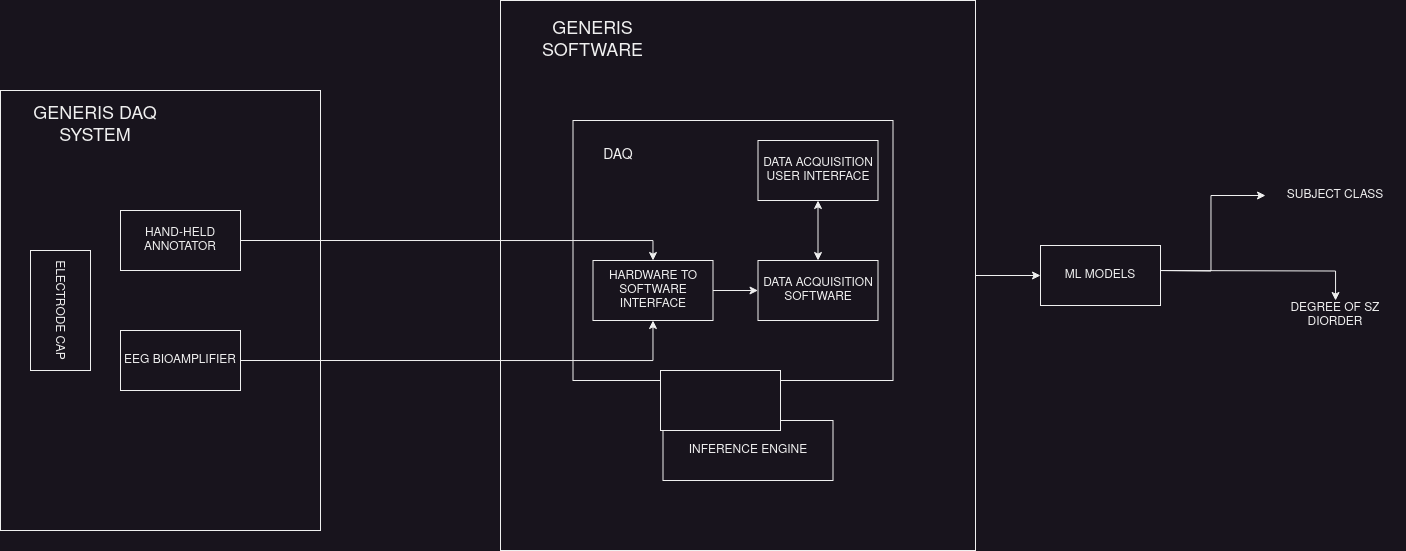
\includegraphics[width=16cm]{../../../images/technical/instrument.drawio.png}
  \caption{\gls{sz} diagnosis instrument}\label{instrument}
\end{figure}


\section{Handheld clicker}
The handheld clicker design is based on an arduino nano which applies the output of four 
tact switches as inputs to four vectored interrupts on the nano development board. The 
exact labels of these inputs has not been assigned as a study of the erogonomics of 
conventions employed in other devices of this kind and how best conventions are adapted and 
modified for the use case of this project is being studied. 

The current design of the handheld clicker(annotator) is the second iteration and is referred 
to as HC-v0.2. 
The circuit diagram of the handheld clicker is given in figure \ref{clicker_circuit}.
The flowchart describing the algorithm of this device is shown in figure \ref{clicker_flowchart}. 
The front and top images of the hand-clicker-v0.2 are shown in figures \ref{clicker} and 
\ref{top_view_of_clicker}.
\begin{figure}[H]
  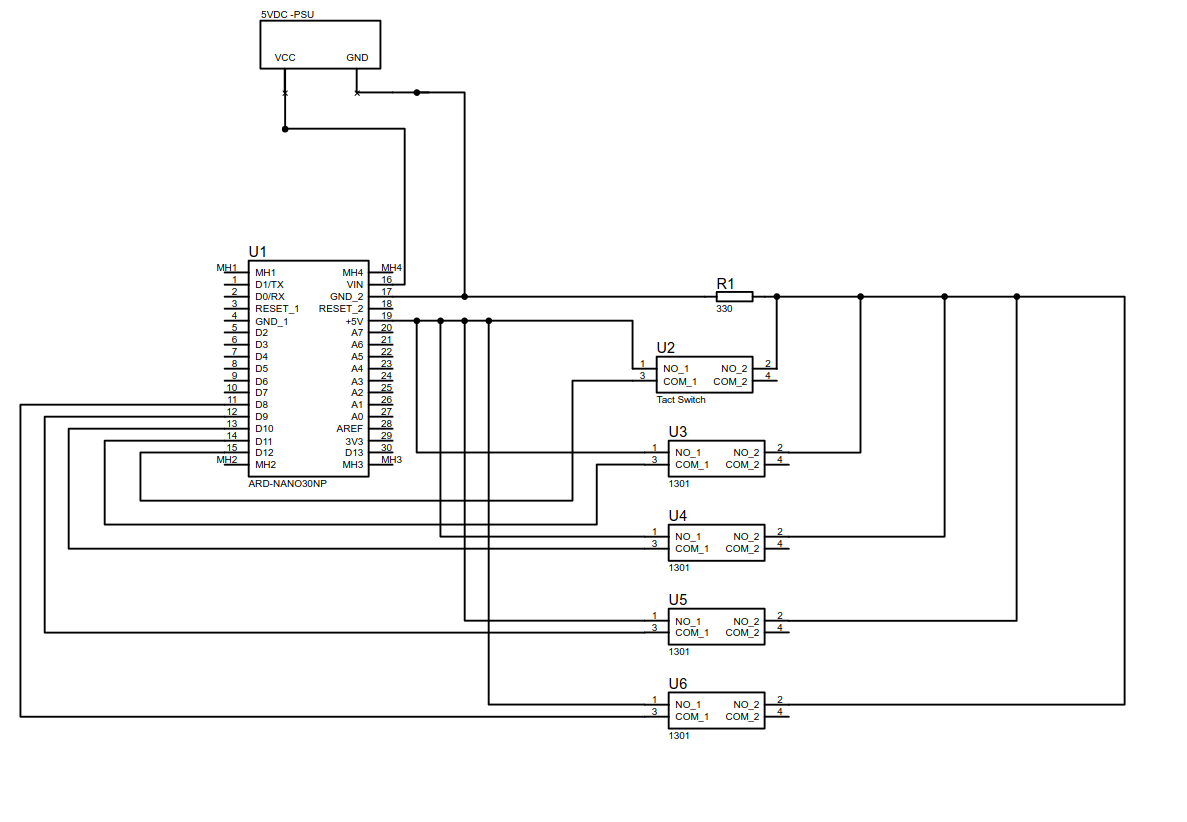
\includegraphics[width=16cm]{../../../hardware/handheld_clicker/circuit_image.png}
  \caption{handheld clicker circuit}\label{clicker_circuit}
\end{figure}
\begin{figure}[H]
  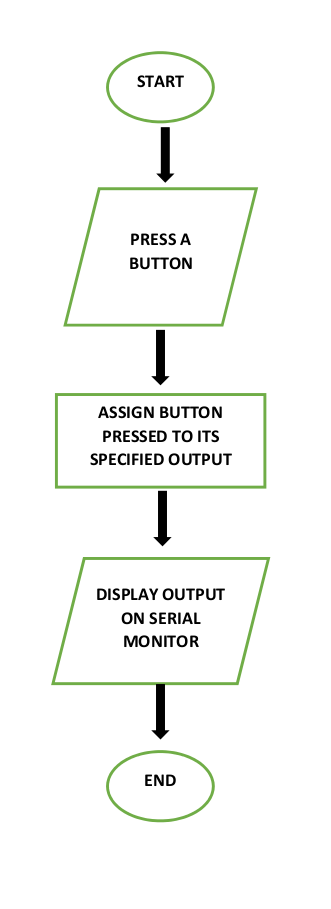
\includegraphics[height=16cm,width=10cm]{../../../hardware/handheld_clicker/flowchart.png}
  \caption{Flowchart algorithm of clicker}\label{clicker_flowchart}
\end{figure}
\begin{figure}[H]
  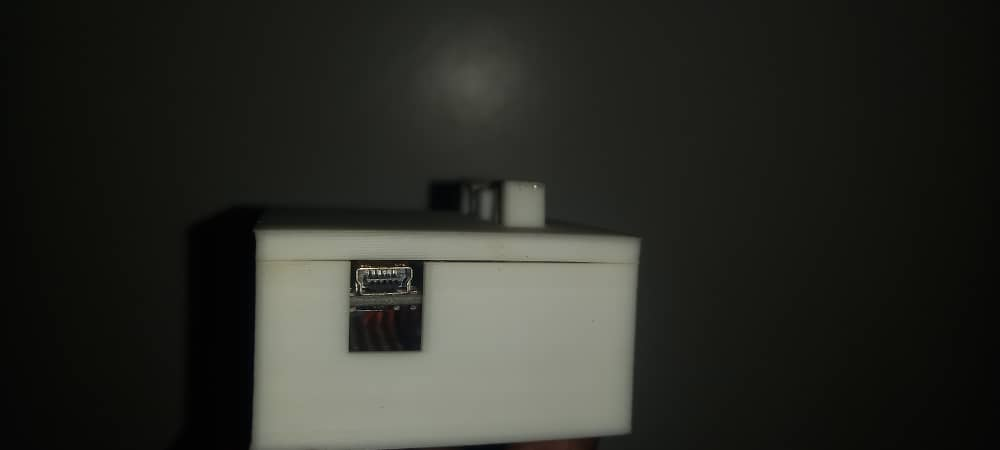
\includegraphics[width=16cm]{../../../hardware/handheld_clicker/front.jpeg}
  \caption{Front view of clicker}\label{clicker}
\end{figure}
\begin{figure}[H]
  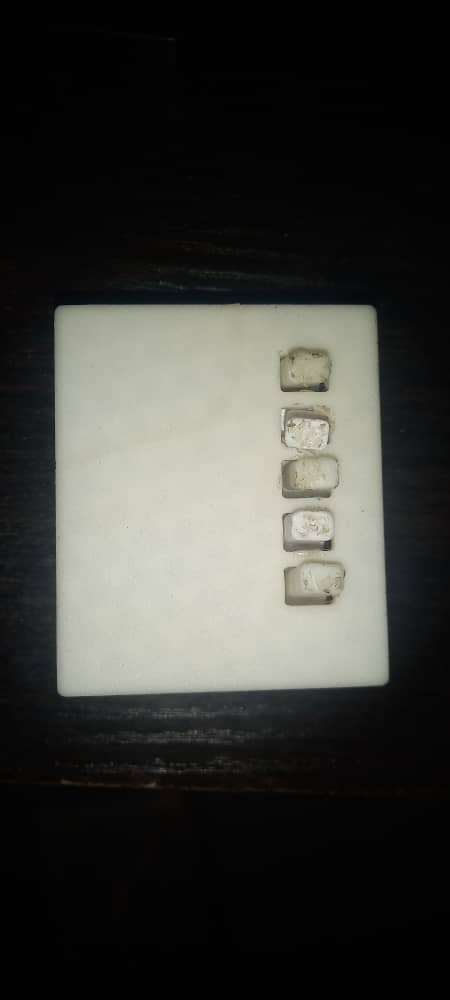
\includegraphics[,height=10cm,width=8cm]{../../../hardware/handheld_clicker/top.jpeg}
  \caption{Top view of clicker}\label{top_view_of_clicker}
\end{figure}


\section{Model Development (Feature-extraction, Data-analysis)}
\subsection{Feature Extraction}
March's report presented the fuzzy entropy features extracted from cortical
regions during phases of \gls{daq} and also the refined \gls{mmn} plots which 
made the \gls{mmn} waveform more evident. Relevant changes made to features 
extraction highlighted in marchs's report includes:
\begin{itemize}
  \item Recomputing the \gls{mmn} waveforms
  \item Spatial dimension augmentation with gaussian noise during computation of fuzzy-entropy
  \item Development of custom fuzzy-entropy library
\end{itemize}
The following was proposed as the next set of action points:
\begin{itemize}
  \item The continued improvement of fuzzy-entropy library to work with multivariate \\
  time-series(2D data)
  \item comparing performance of the fuzzy-entropy features from sourced library to \\
  that of the personally developed library
  \item Computing the auditory steady state features
\end{itemize}
A slight detour was made from these proposed action points for the month of april. 
Analysis of the extracted features for levels of dicriminability was carried out 
to understand how to improve the features extraction methods. The analysis shows 
a significant level of discrimination in the \gls{mmn} features, less in the 
fuzzy-entropy features, though the correlation patterns of the fuzzy-entropy features 
suggest they might carry information on extent of \gls{sz} disorder.

\gls{mmn} features have been extracted from the scaled \gls{mmn} waveforms. The 
\gls{mmn} features were computed as the mean of the \gls{mmn} waveforms within 
the time-frames 0-100ms, 100-200ms, 200-300ms, 300-400ms, 400-450ms.

Formerly implemented montage plot algorithm was improved upon to reduce 
time-complexity so as to make data visualization and analysis easier to obtain 
intuitive information from.

\subsection{Data Analysis/Visualization}\label{data_analyis}
 Analysis of the extracted features was done to establish the quality of discriminative 
 and quantitative information contained in the extracted features. The method of 
 Visualization of some of these features changed to make analysis easy.
 The results of the analysis are given in section \ref{figures}. Visualization methods 
 and analysis carried out includes:
\begin{itemize}
  \item Comparing \gls{mmn} feature values for 1KHz duration deviant and 3KHz frequency deviant 
  between patient and controls across all electrodes and time windows.
  (Figures \ref{mmnvalue_0_100ms} - \ref{mmnvalue_400_450ms})
  \item Converting the \gls{mmn} values to montage plots for 1KHz duration deviant 
  and 3KHz frequency deviant for easier interpretation and analyzing montage evolution.
  (Figures \ref{control_1KHz_mmn_montage}-\ref{patient_3KHz_mmn_montage})
  \item Comparing distribution of computed fuzzy-entropy values of patients and controls 
  for each cortical region across all phases of \gls{daq}.
  (Figures \ref{fig:controlFuzzEnt}-\ref{fuzz_ent_distributions}) 
  \item Correlating fuzzy-entropy values from cortical regions across 
  all phases of \gls{daq}.(Figure \ref{fuzz_ent_corr_mat})
  \item Comparing entropies from all cortical regions for each phase of \gls{daq}.
  (Figures \ref{rest_fuzz}-\ref{auditory_fuzz})
  \item Comparing entropies from all phases of \gls{daq} for each cortical region.
  (figures \ref{frontal_fuzz}-\ref{temporal_fuzz})
\end{itemize} 

\section{Inference and Action Points}
\subsection{Inference}
From the analysis carried out, the \gls{mmn} features of both tone deviants show 
discriminative properties between the \gls{szPtnt} and \gls{hc} in localized head 
regions. The fuzzy-entropy features do not show discriminative abilities, but their 
correlation patterns indicate a linear relationship that might be a measure of degree 
of \gls{sz} disorder. Therefore we need to find methods that improve quality of extracted 
features and proceed with developing a learner model.

\subsection{Action Points}
Based on the inference drawn, the action points for the month of may is as follows:
\begin{itemize}
  \item Computing the auditory steady state features.
  \item Re-computing fuzzy-entropy features using other libraries and 
  comparing performance.
  \item Improve discriminability of features using spatial filters and dimensionality 
  reduction techniques.
  \item Compare performance of a custom mutilayer feedforward network and traditional 
  machine-learning algorithms for classification and estimation of measures of degree 
  of \gls{sz} disorder.
\end{itemize}

\section{Figures}\label{figures}

\begin{figure}[H]
  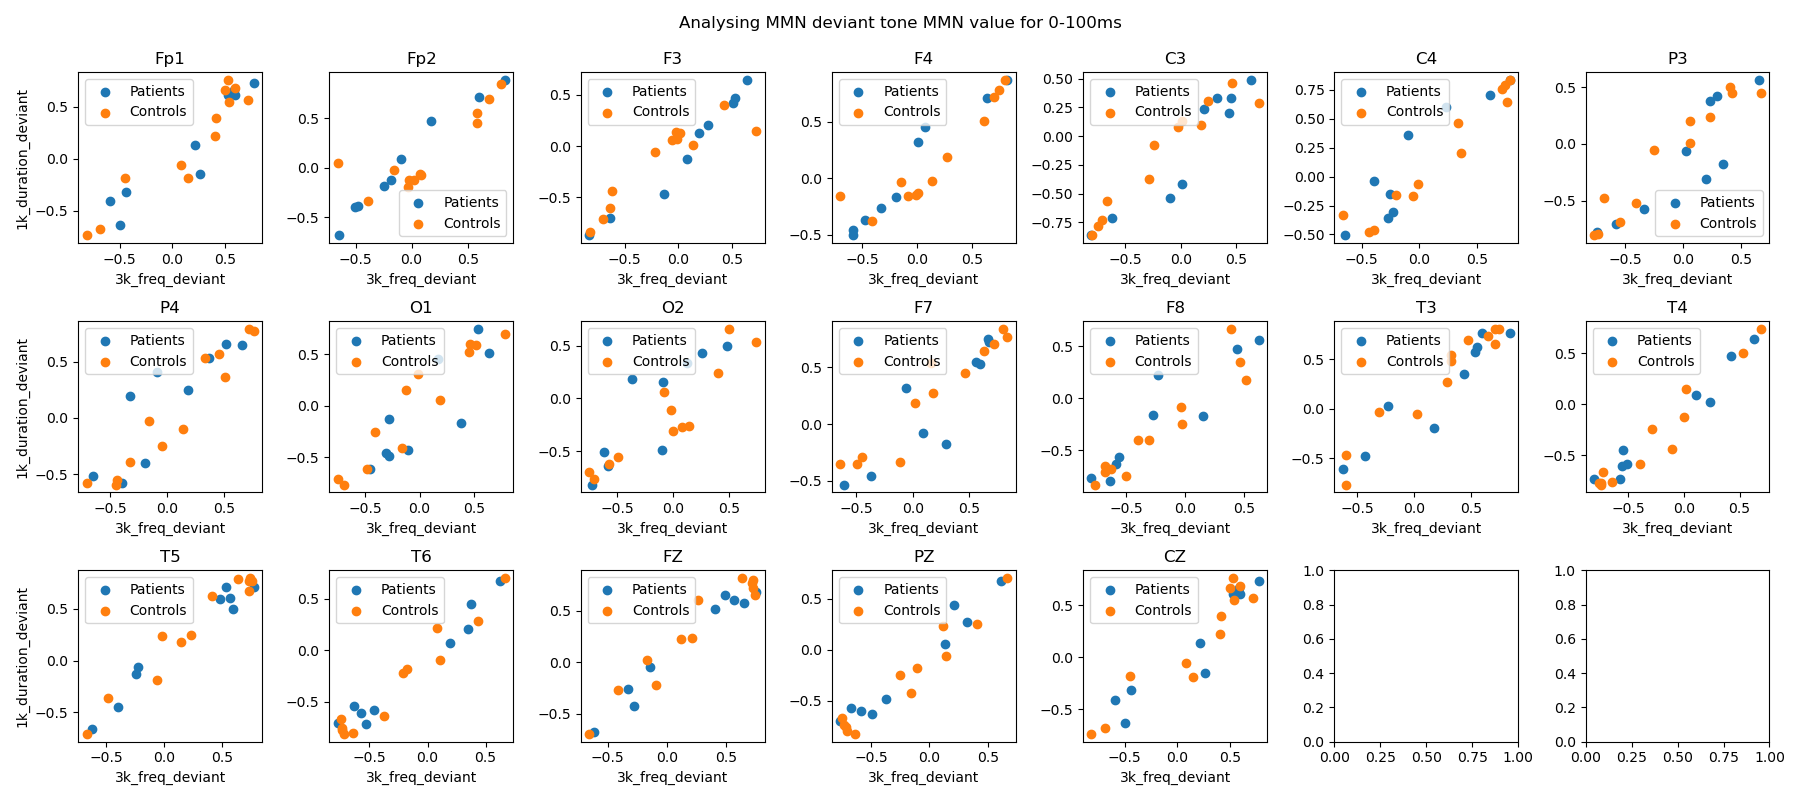
\includegraphics[width=16cm]{../../../data_analysis_results/MMN/features/deviant_tone_0.png}
  \caption{\gls{mmn} values from 0-100ms}\label{mmnvalue_0_100ms}
\end{figure}
\begin{figure}[H]
  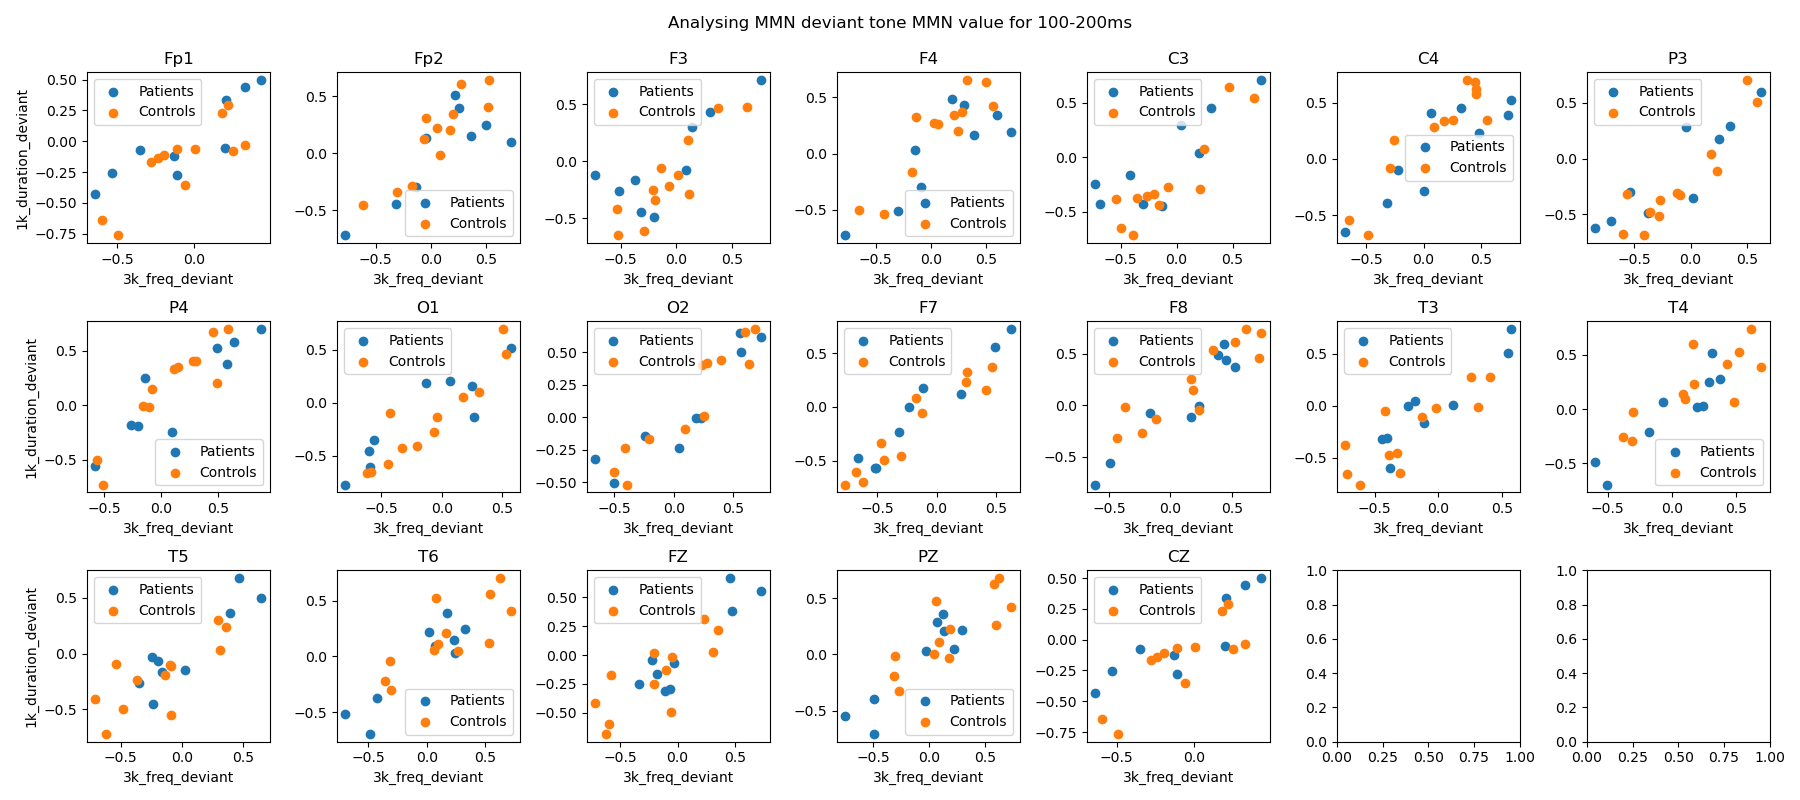
\includegraphics[width=16cm]{../../../data_analysis_results/MMN/features/deviant_tone_1.png}
  \caption{\gls{mmn} values from 100-200ms}\label{mmnvalue_100_200ms}
\end{figure}
\begin{figure}[H]
  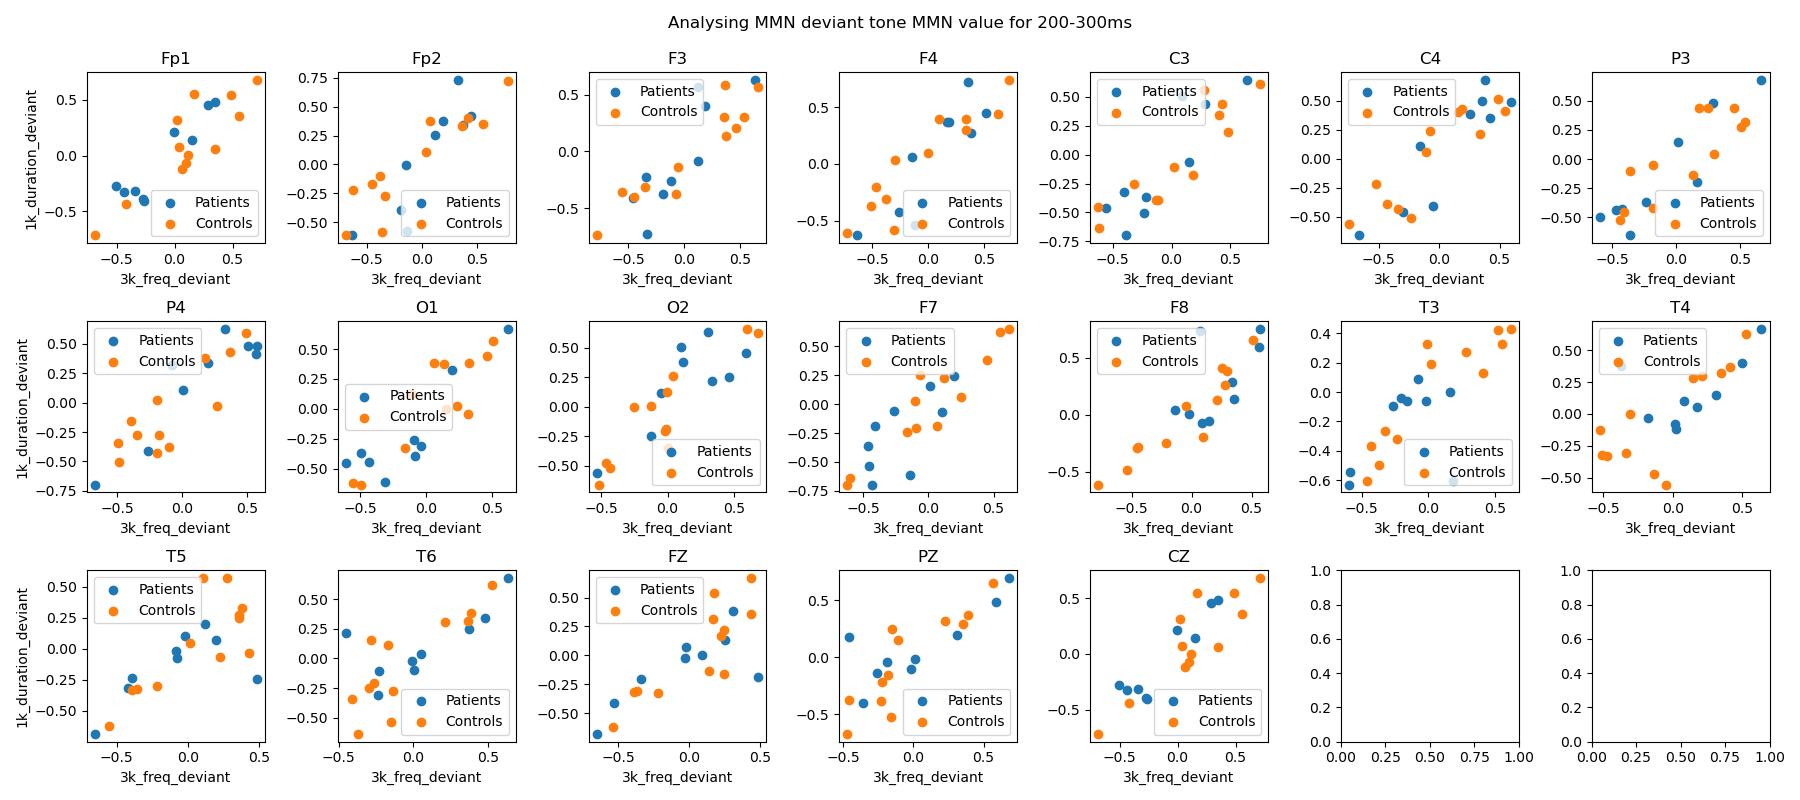
\includegraphics[width=16cm]{../../../data_analysis_results/MMN/features/deviant_tone_2.png}
  \caption{\gls{mmn} values from 200-300ms}\label{mmnvalue_200_300ms}
\end{figure}
\begin{figure}[H]
  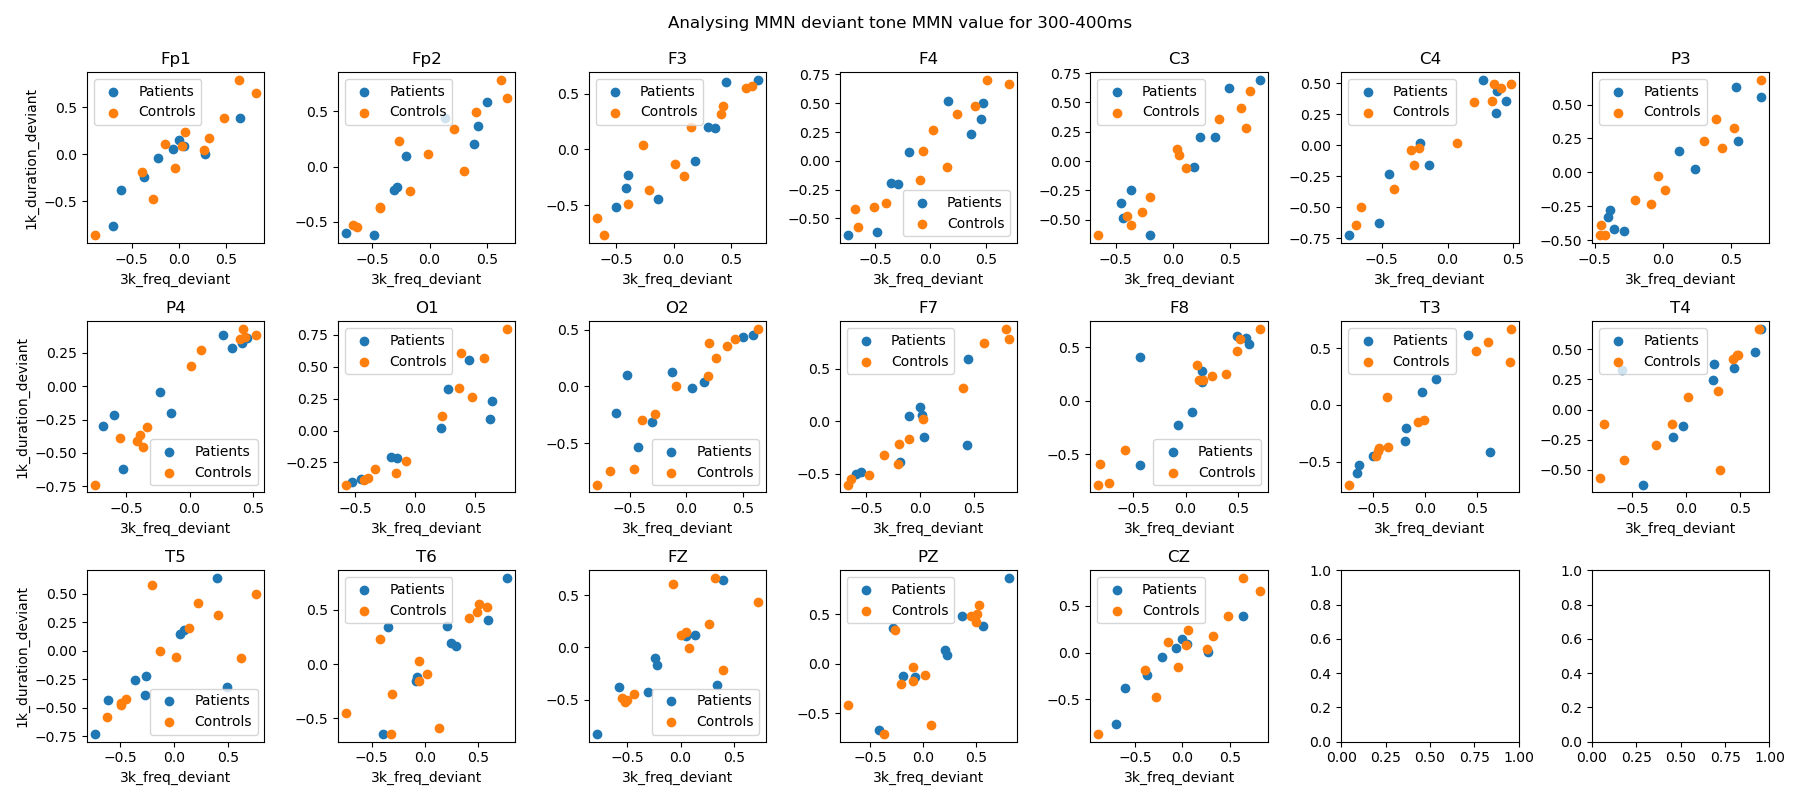
\includegraphics[width=16cm]{../../../data_analysis_results/MMN/features/deviant_tone_3.png}
  \caption{\gls{mmn} values from 300-400ms}\label{mmnvalue_300_400ms}
\end{figure}
\begin{figure}[H]
  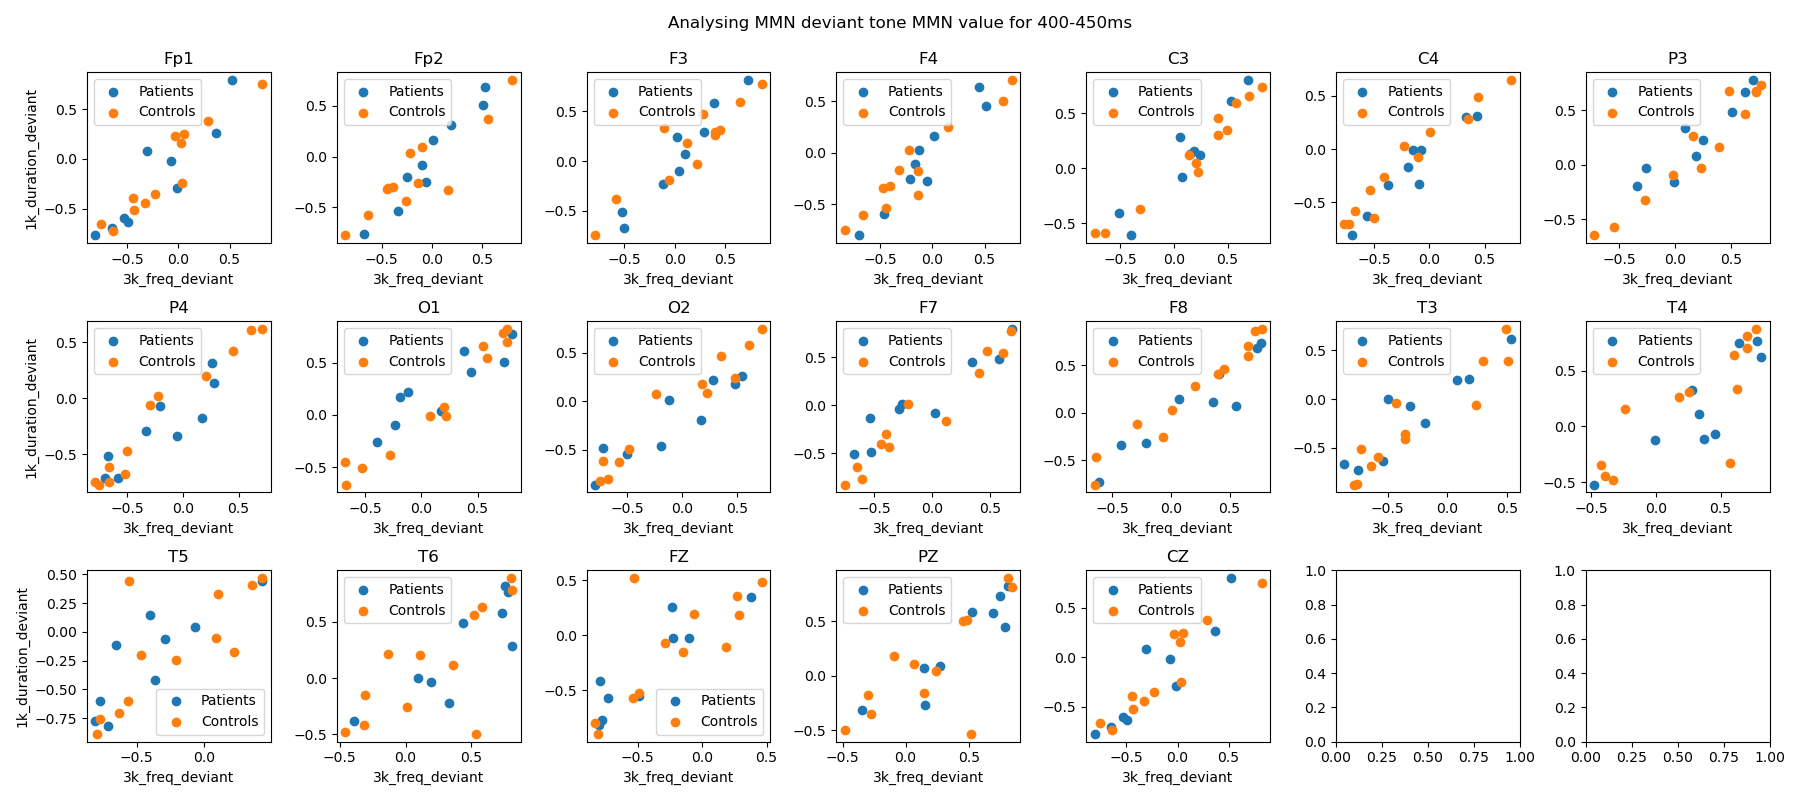
\includegraphics[width=16cm]{../../../data_analysis_results/MMN/features/deviant_tone_4.png}
  \caption{\gls{mmn} values from 400-450ms}\label{mmnvalue_400_450ms}
\end{figure}

\begin{figure}[H]
  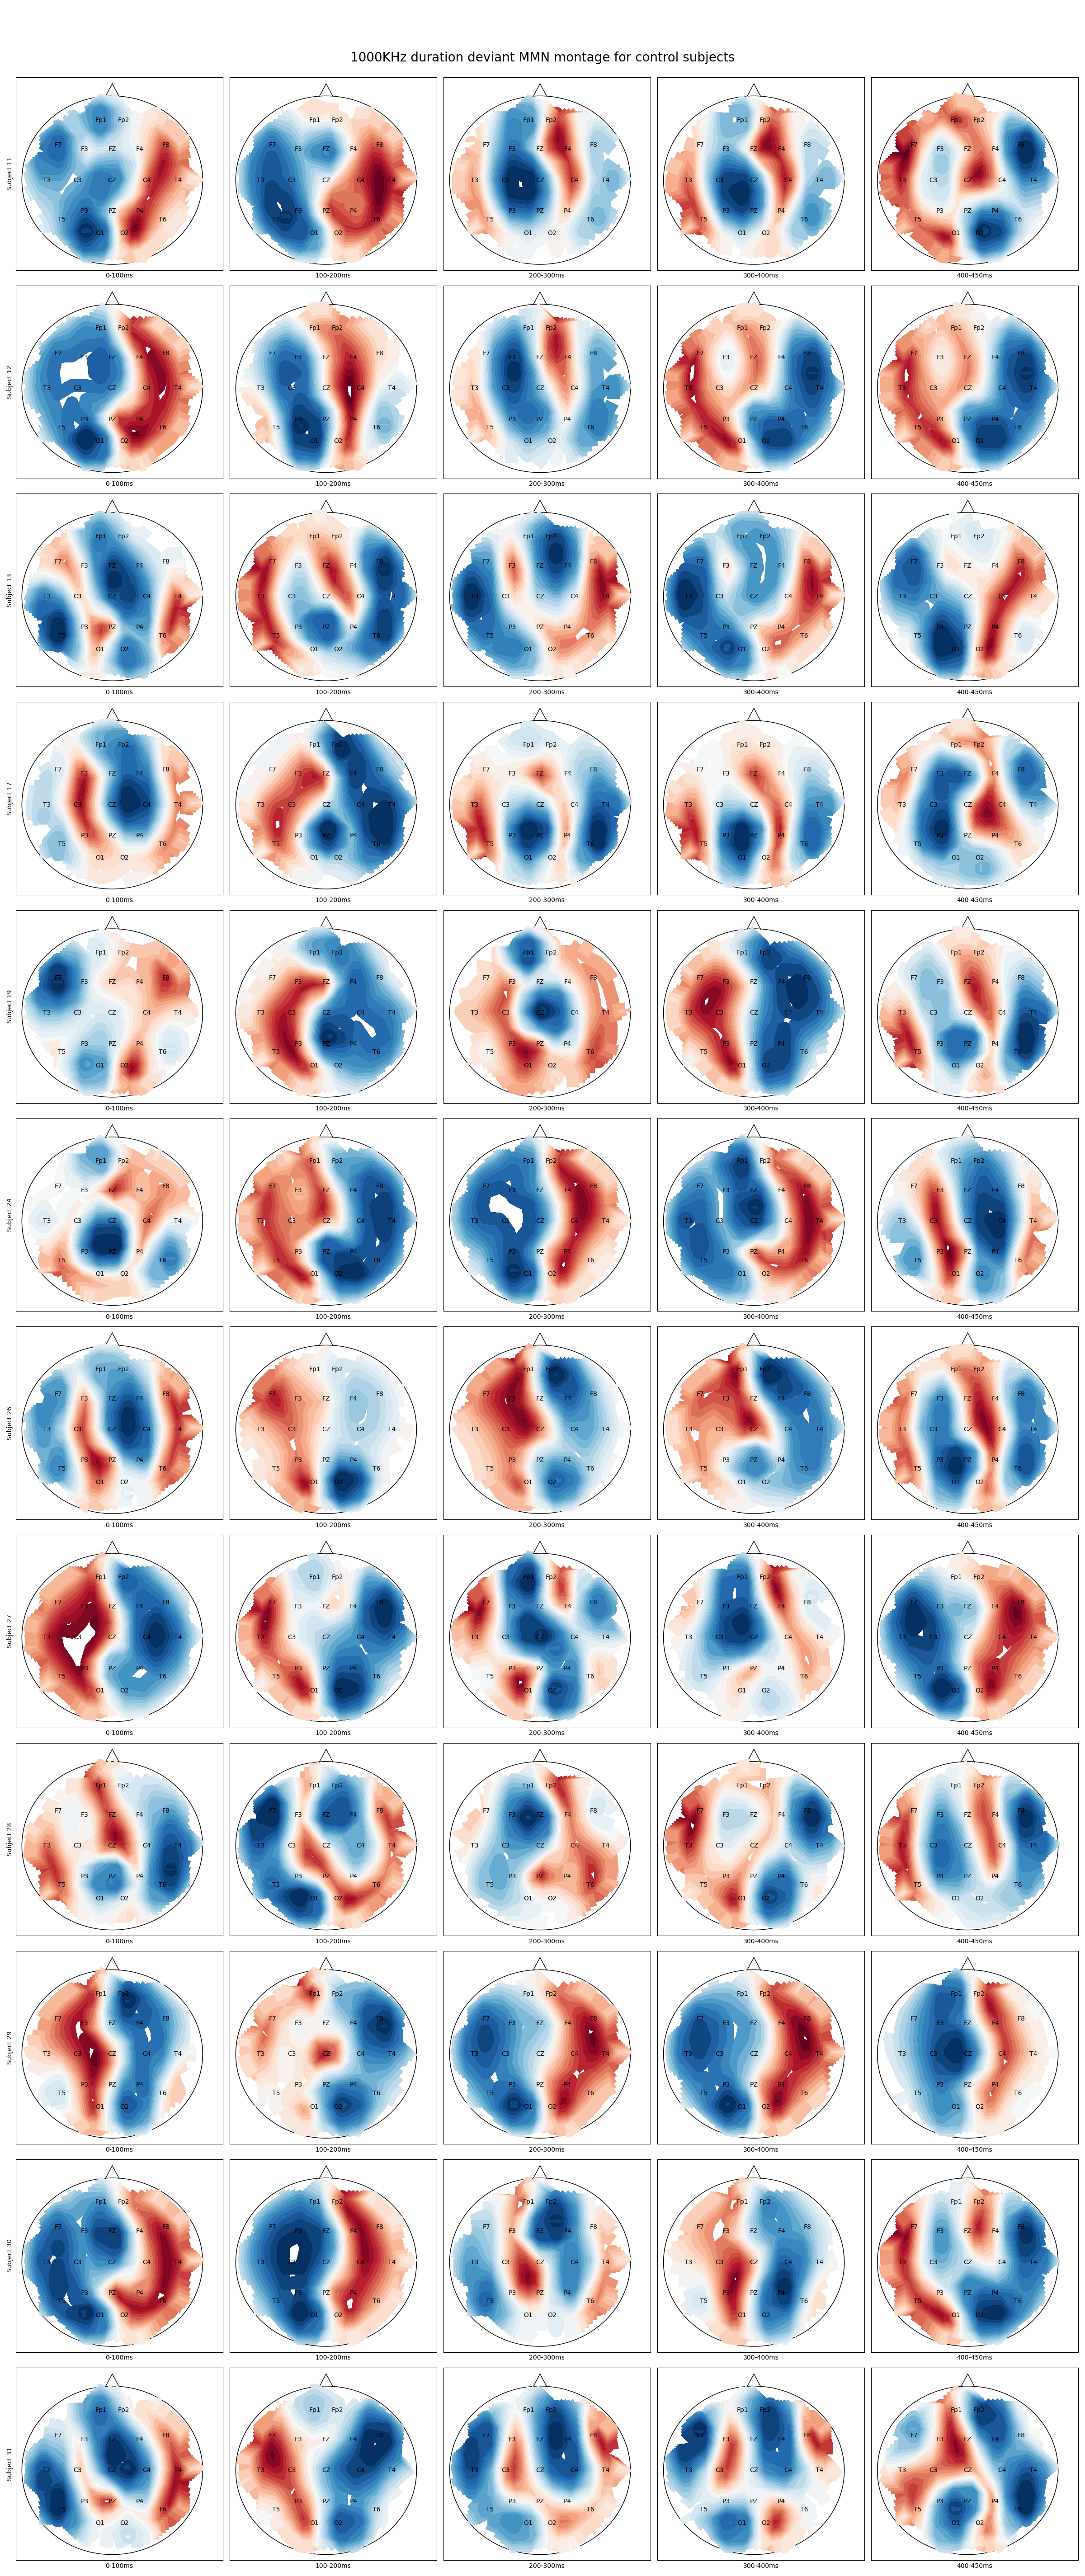
\includegraphics[width=16cm]{../../../data_analysis_results/MMN/montage/Control/1KHz_duration_deviant_montage.png}
  \caption{Controls 1KHz duration deviant \gls{mmn} value montage}\label{control_1KHz_mmn_montage}
\end{figure}
\begin{figure}[H]
  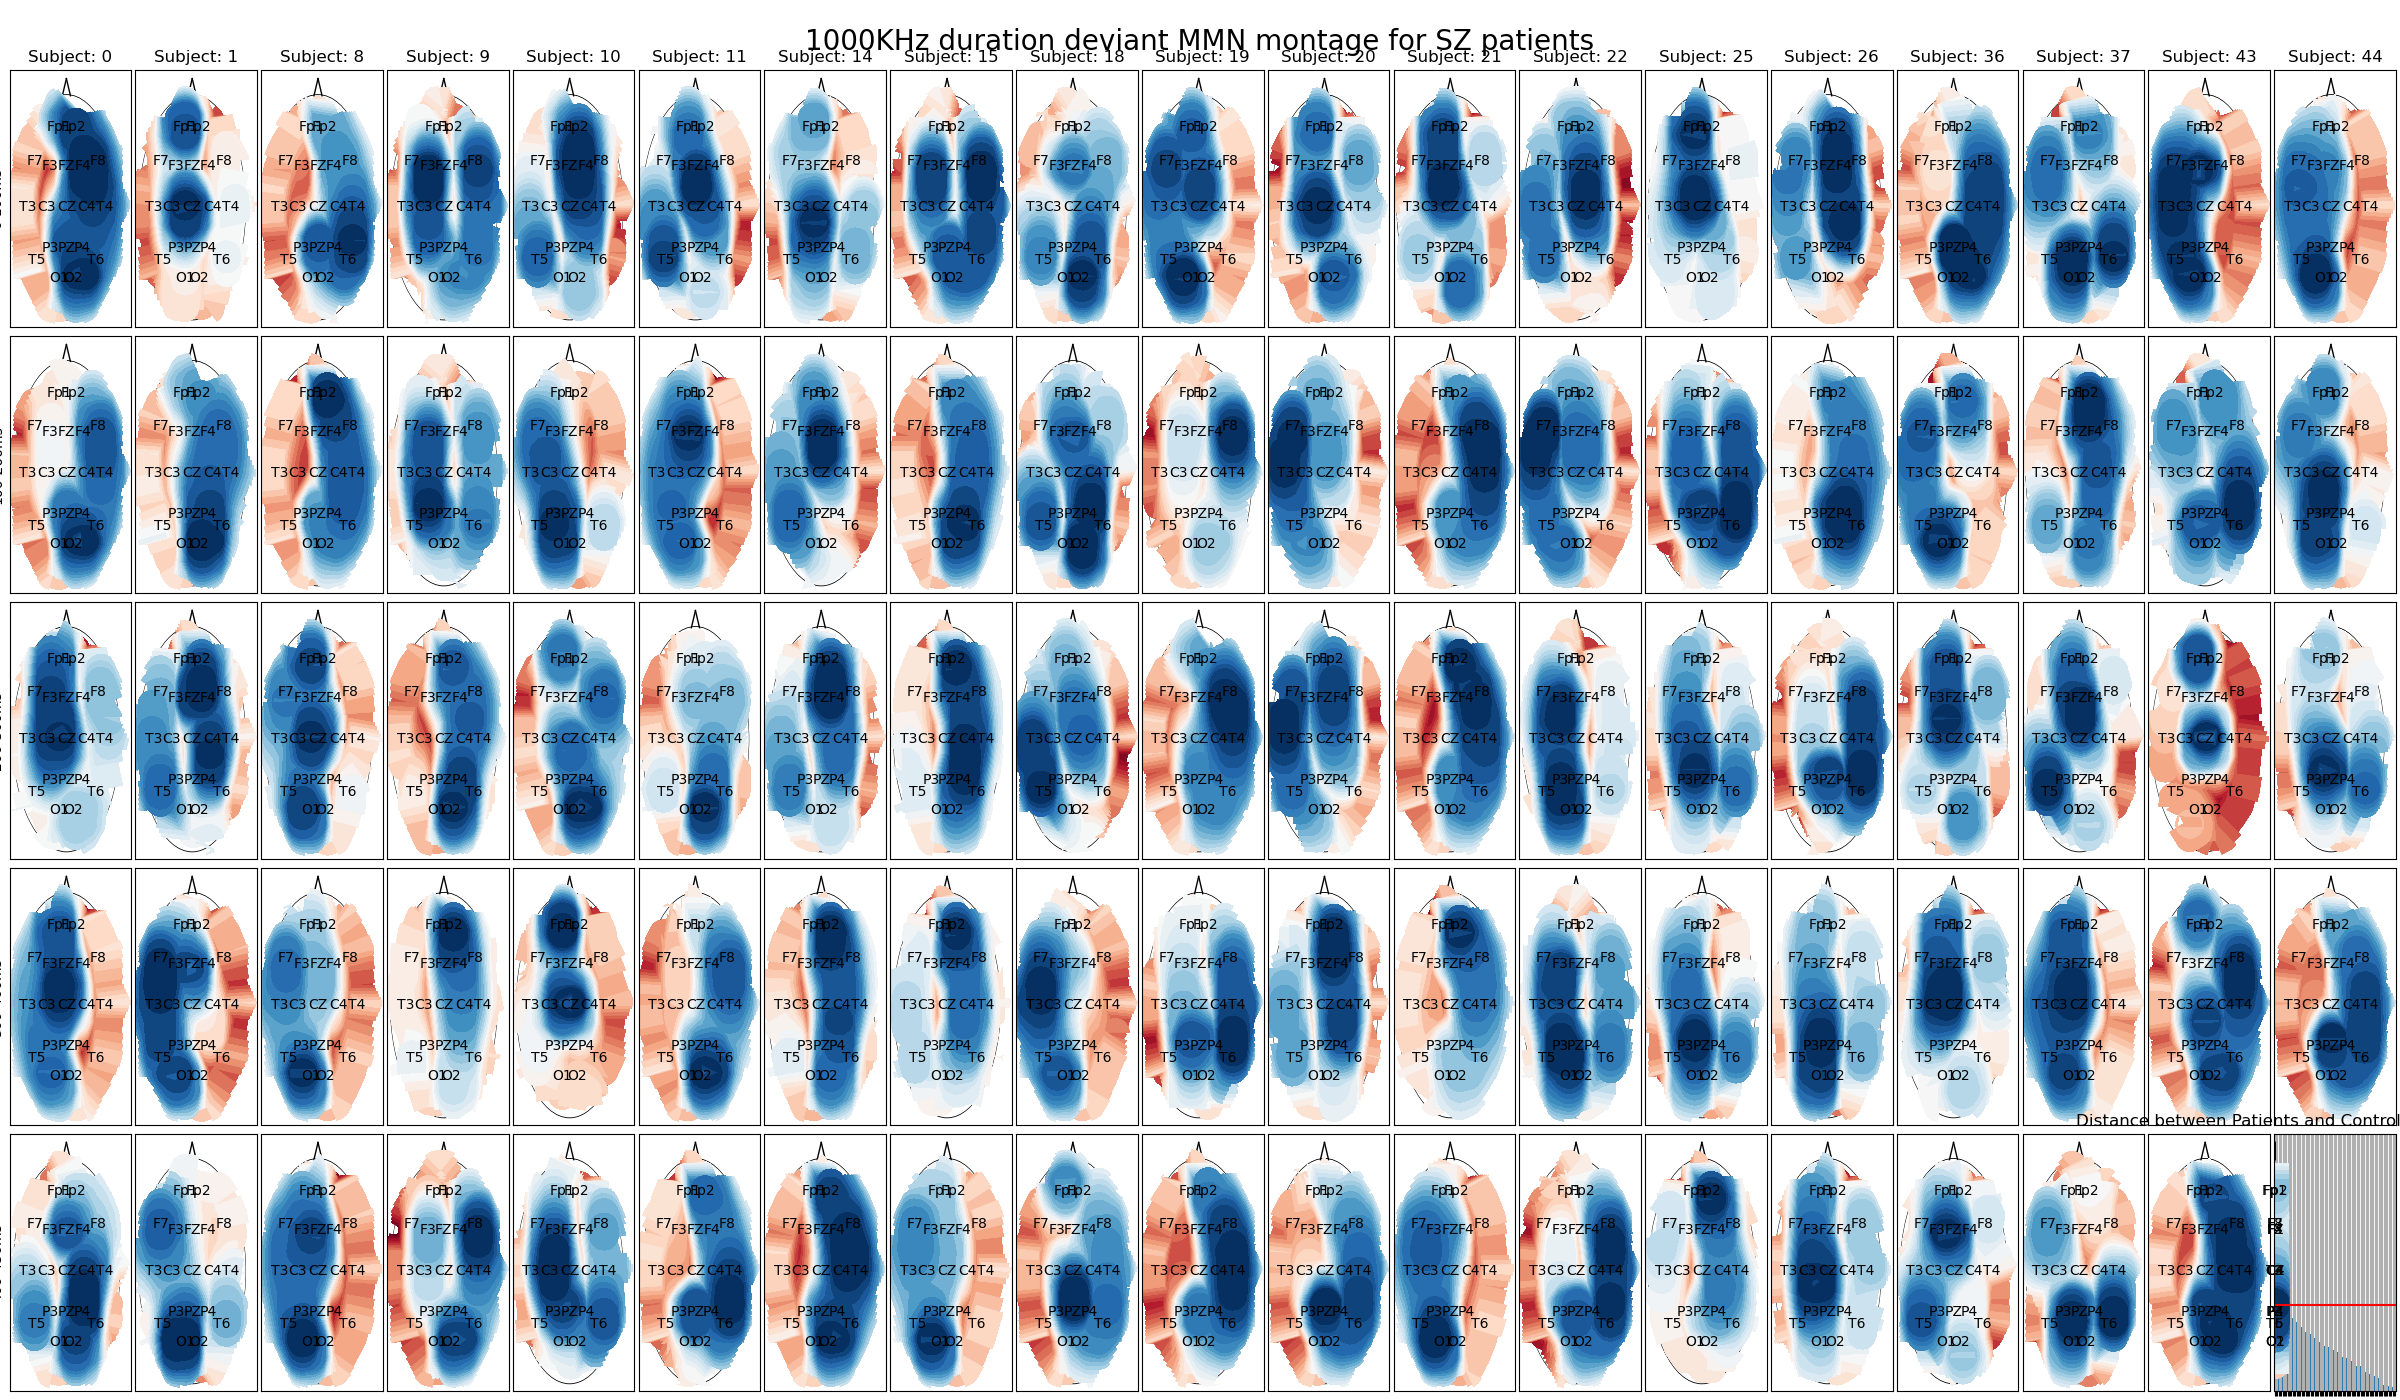
\includegraphics[width=16cm]{../../../data_analysis_results/MMN/montage/Patient/1KHz_duration_deviant_montage.png}
  \caption{Patients 1KHz duration deviant \gls{mmn} value montage}\label{patient_1KHz_mmn_montage}
\end{figure}
\begin{figure}[H]
  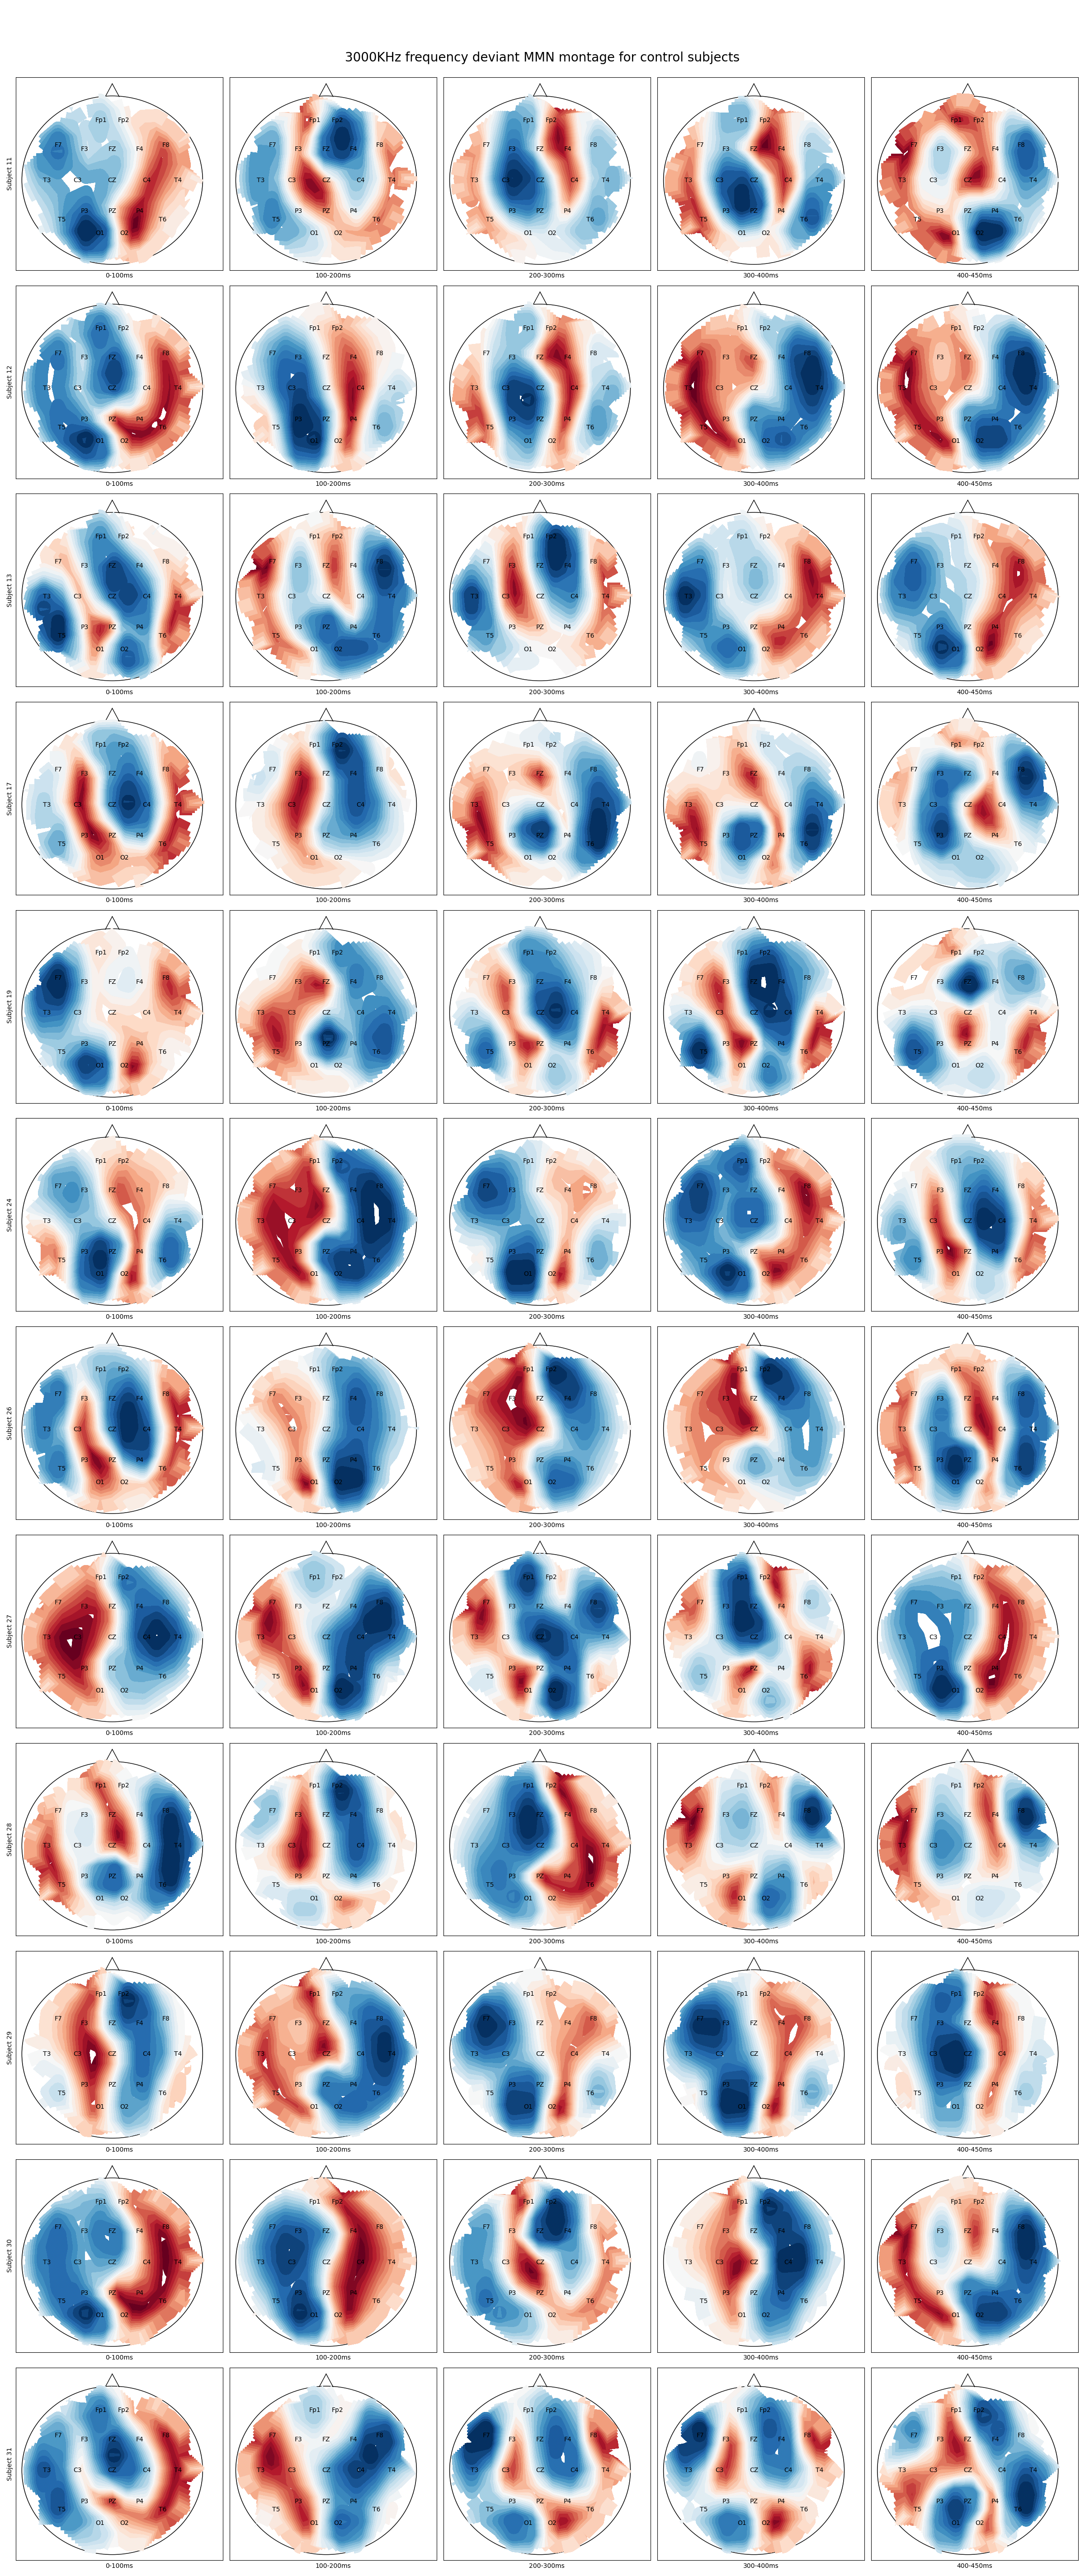
\includegraphics[width=16cm]{../../../data_analysis_results/MMN/montage/Control/3KHz_frequency_deviant_montage.png}
  \caption{Controls 3KHz frequency deviant \gls{mmn} value montage}\label{control_3KHz_mmn_montage}
\end{figure}
\begin{figure}[H]
  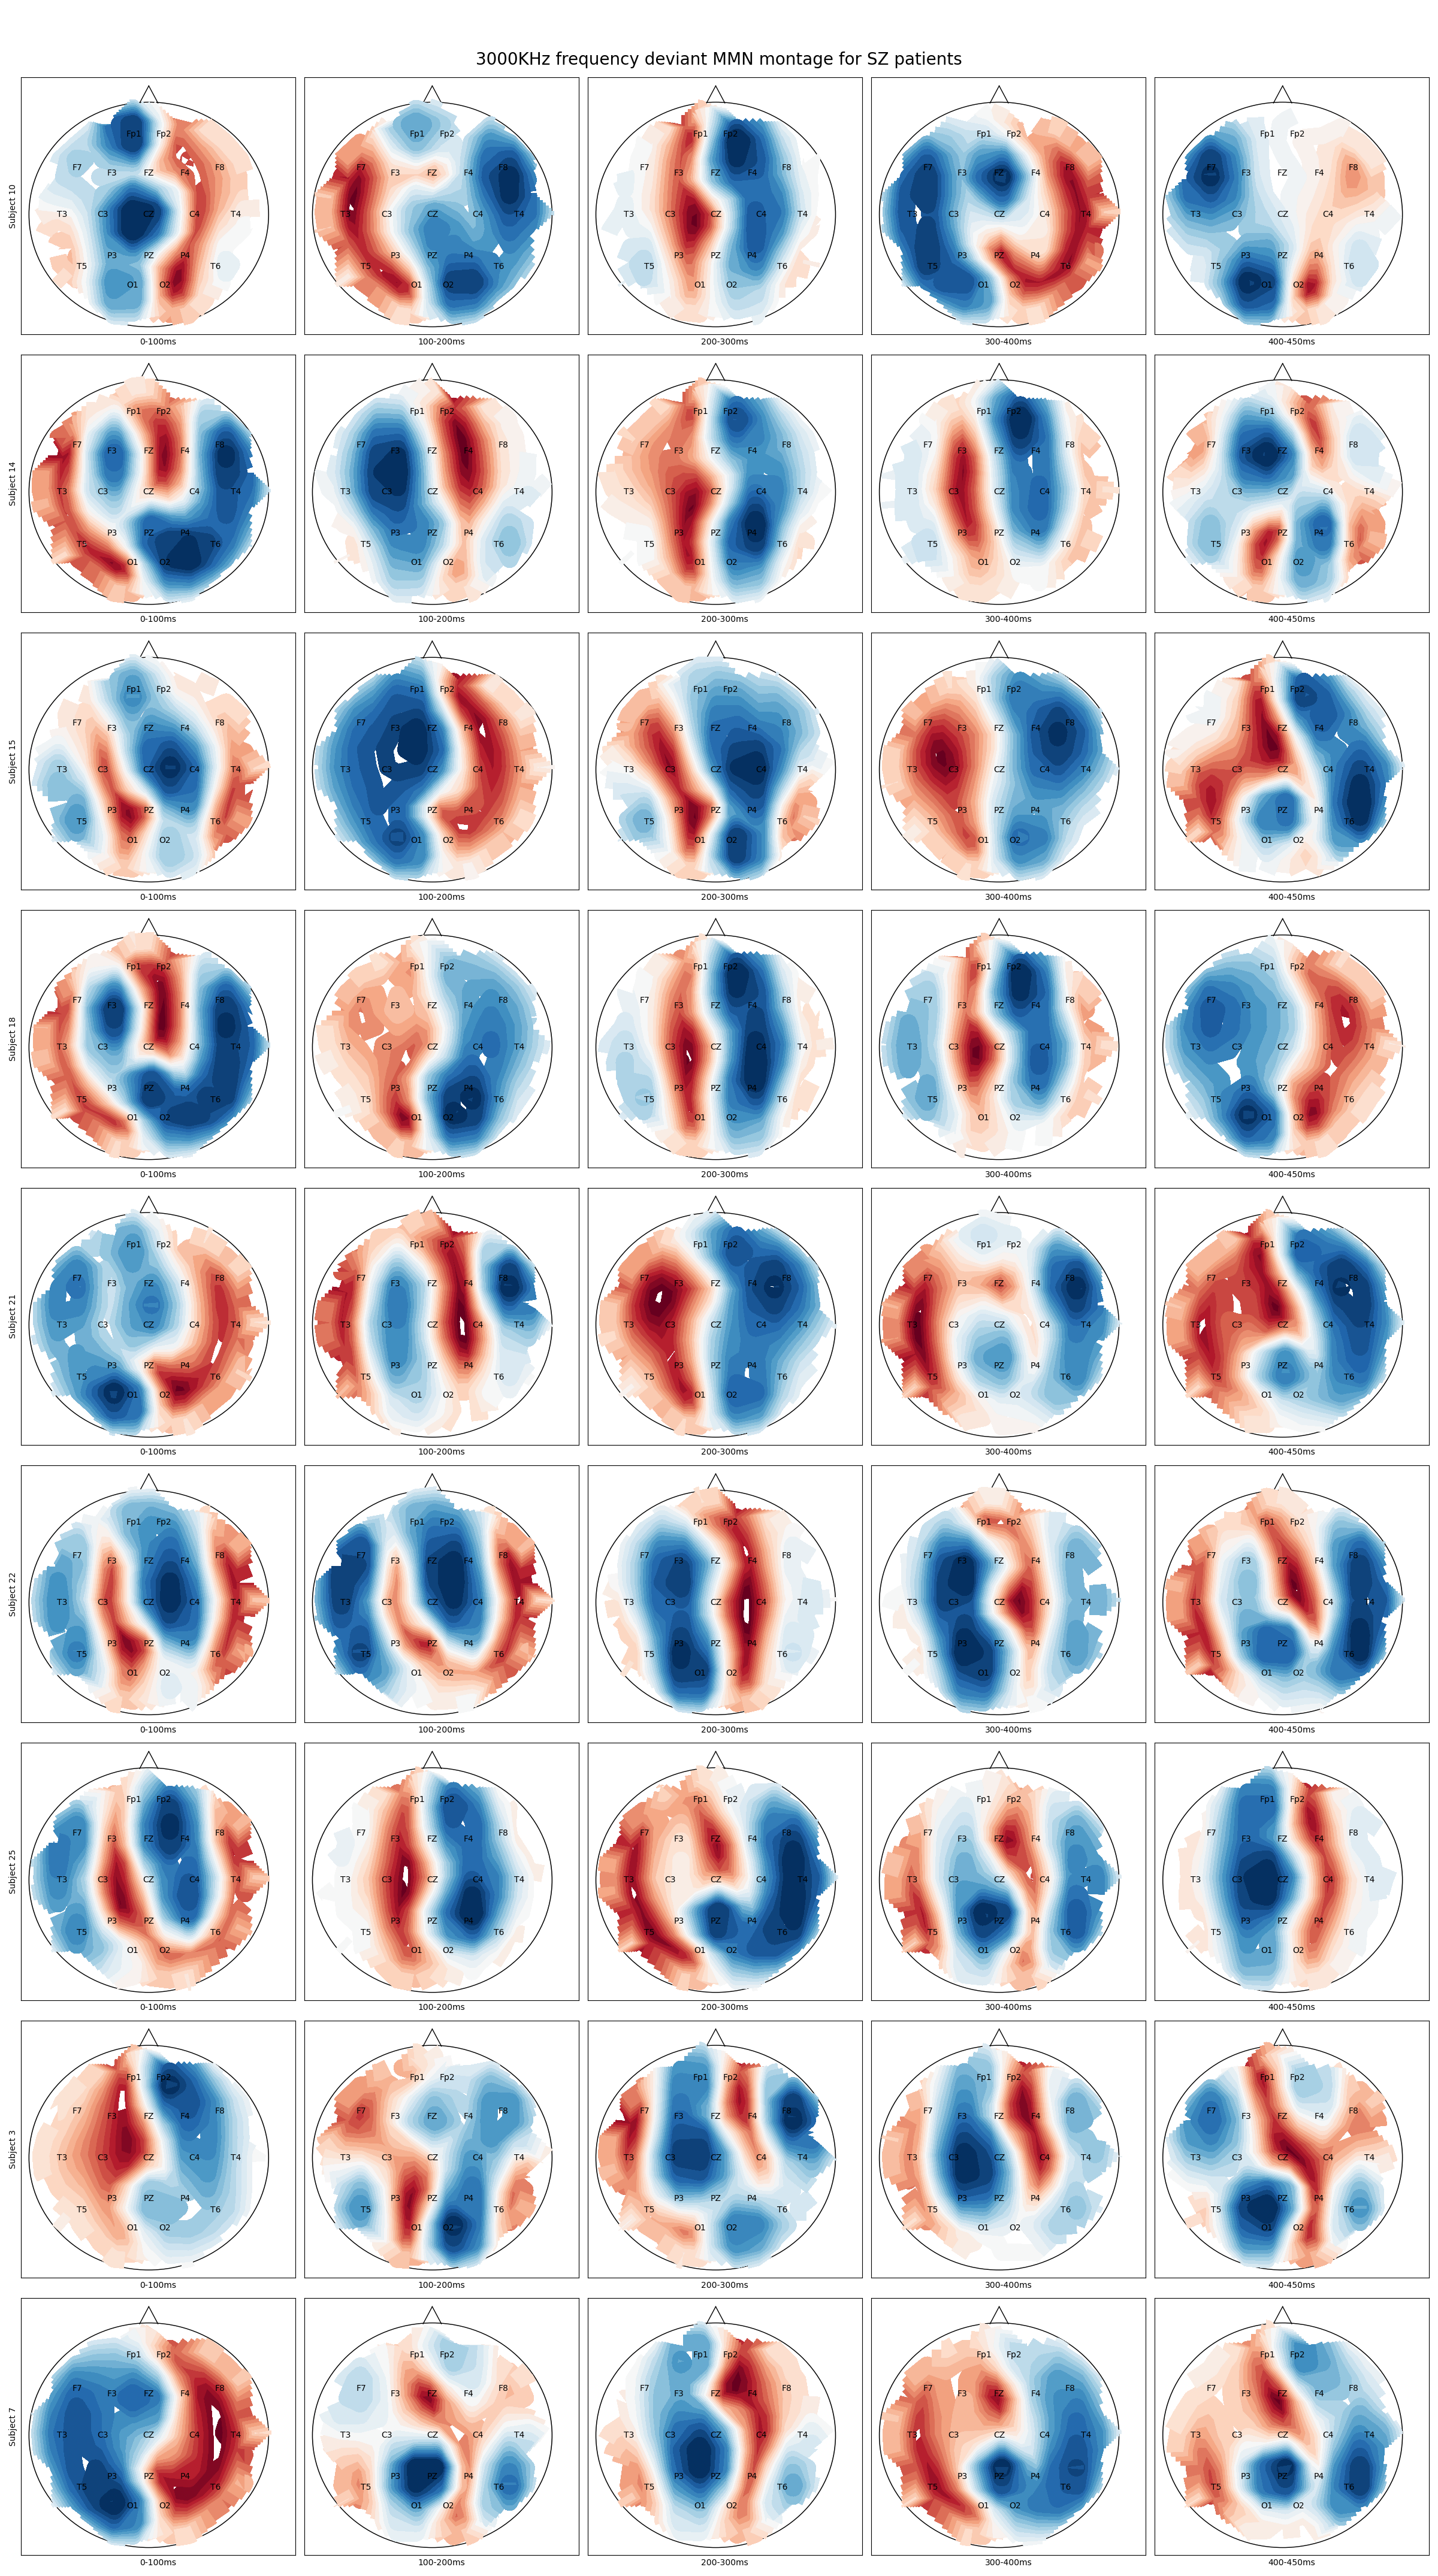
\includegraphics[width=16cm]{../../../data_analysis_results/MMN/montage/Patient/3KHz_frequency_deviant_montage.png}
  \caption{Patients 3KHz frequency deviant \gls{mmn} value montage}\label{patient_3KHz_mmn_montage}
\end{figure}

\begin{figure}[H]
  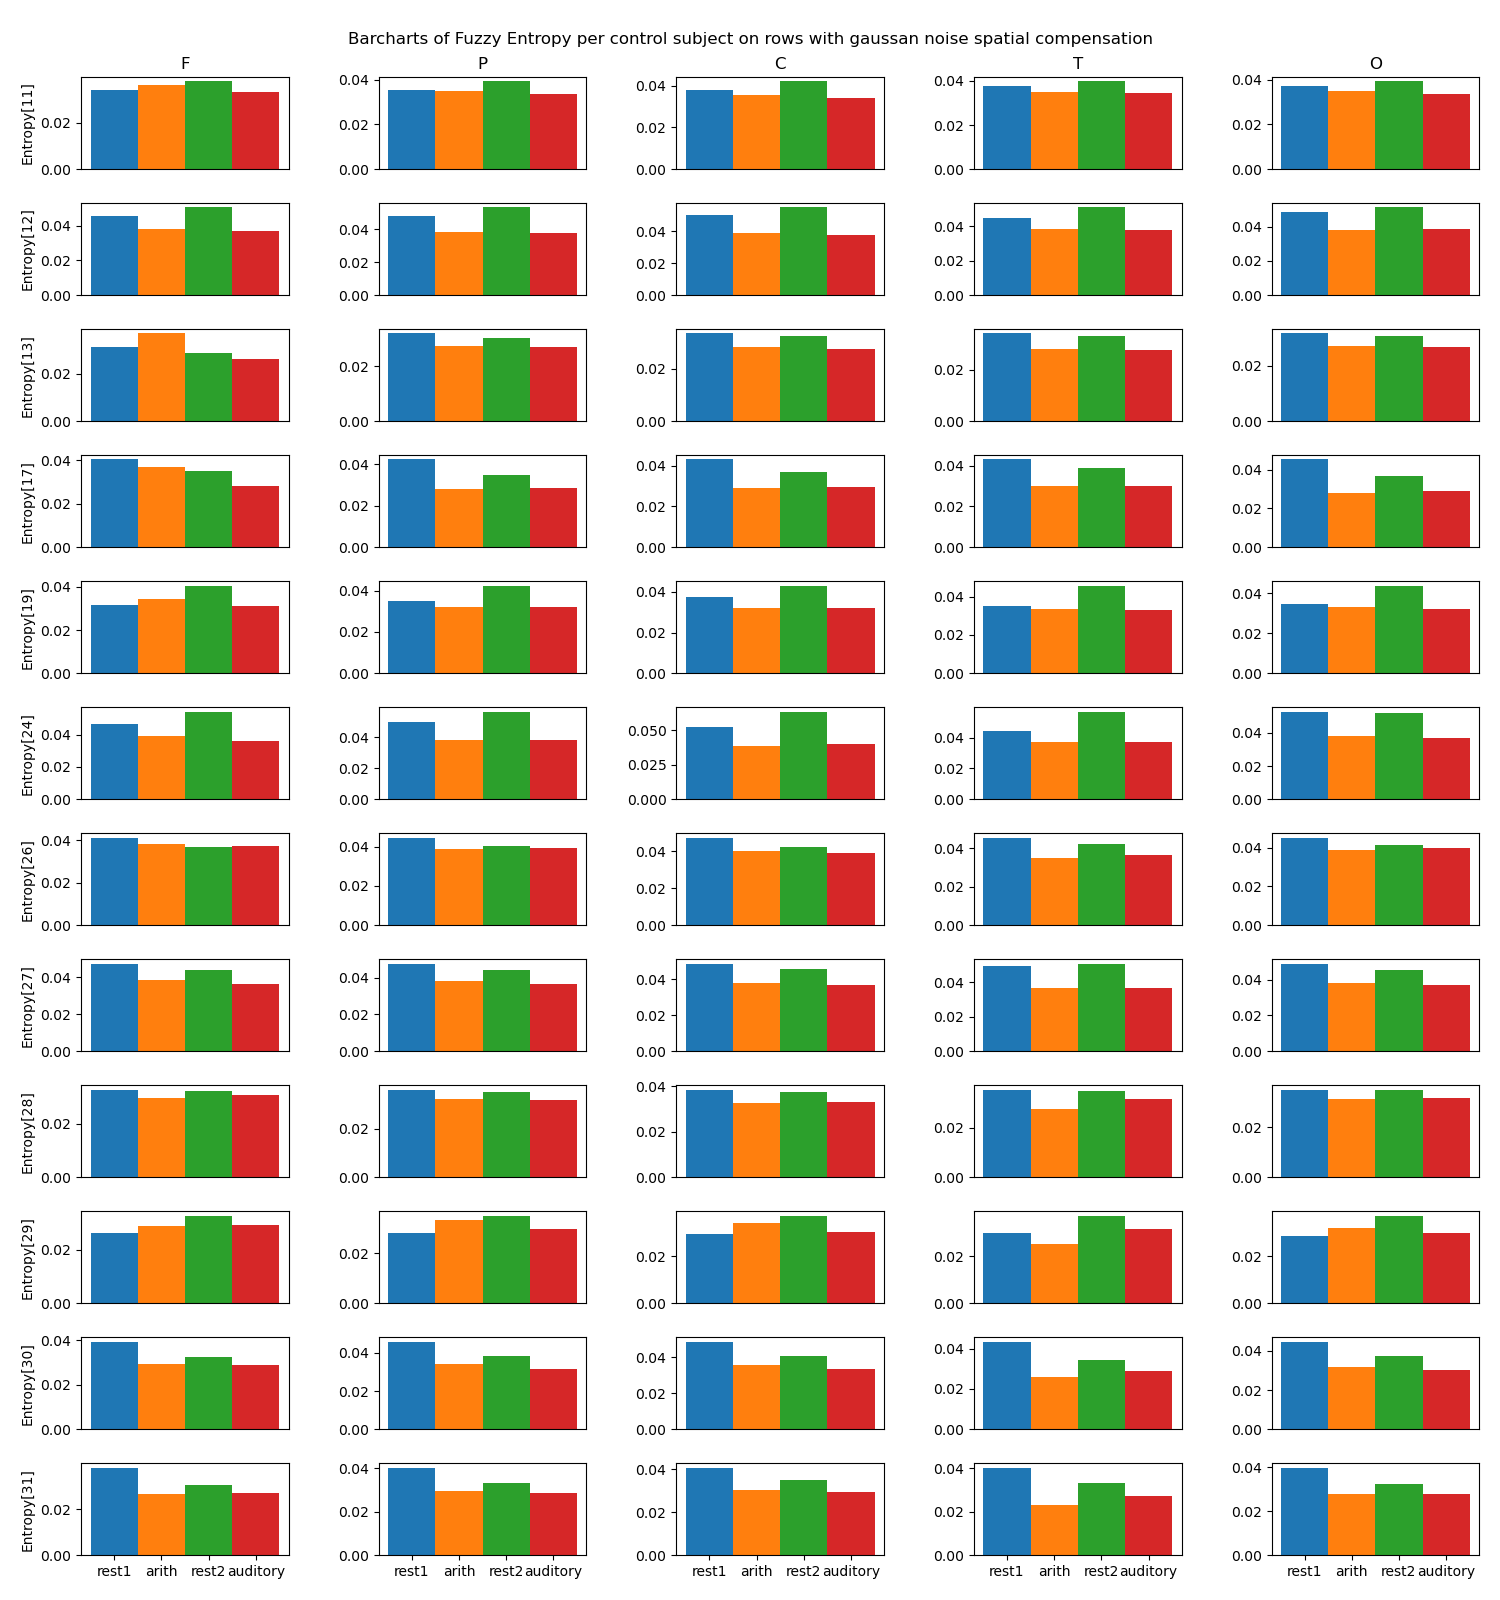
\includegraphics[width=16cm]{../../../data_analysis_results/FuzzEnt/Control/all-fuzzyEntr.png}
  \caption{Fuzzy Entropy from controls}\label{fig:controlFuzzEnt}
\end{figure}
\begin{figure}[H]
  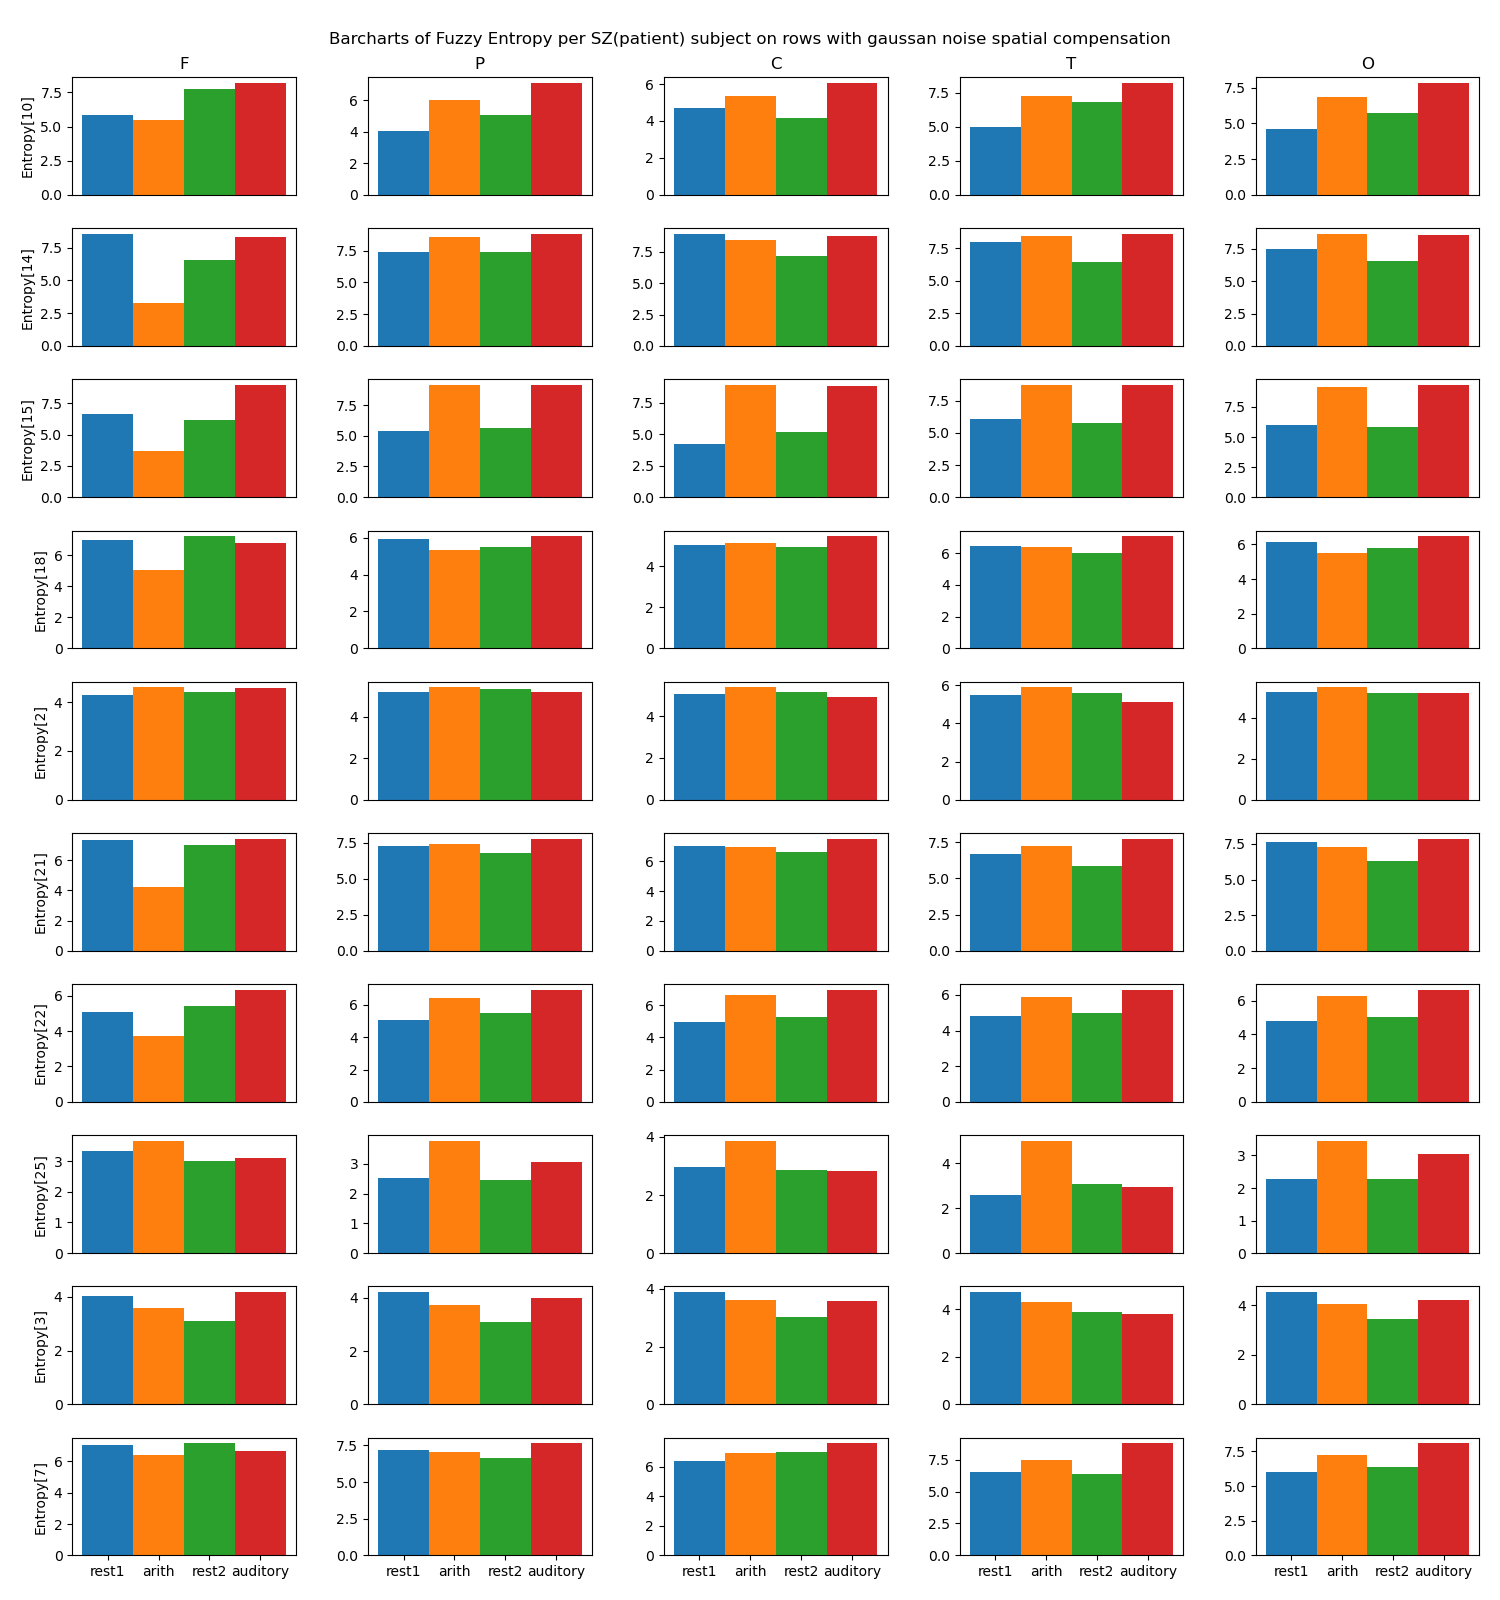
\includegraphics[width=16cm]{../../../data_analysis_results/FuzzEnt/Patient/all-fuzzyEntr.png}
  \caption{Fuzzy Entropy from patients}\label{fig:patientFuzzEnt}
\end{figure}
\begin{figure}[H]
  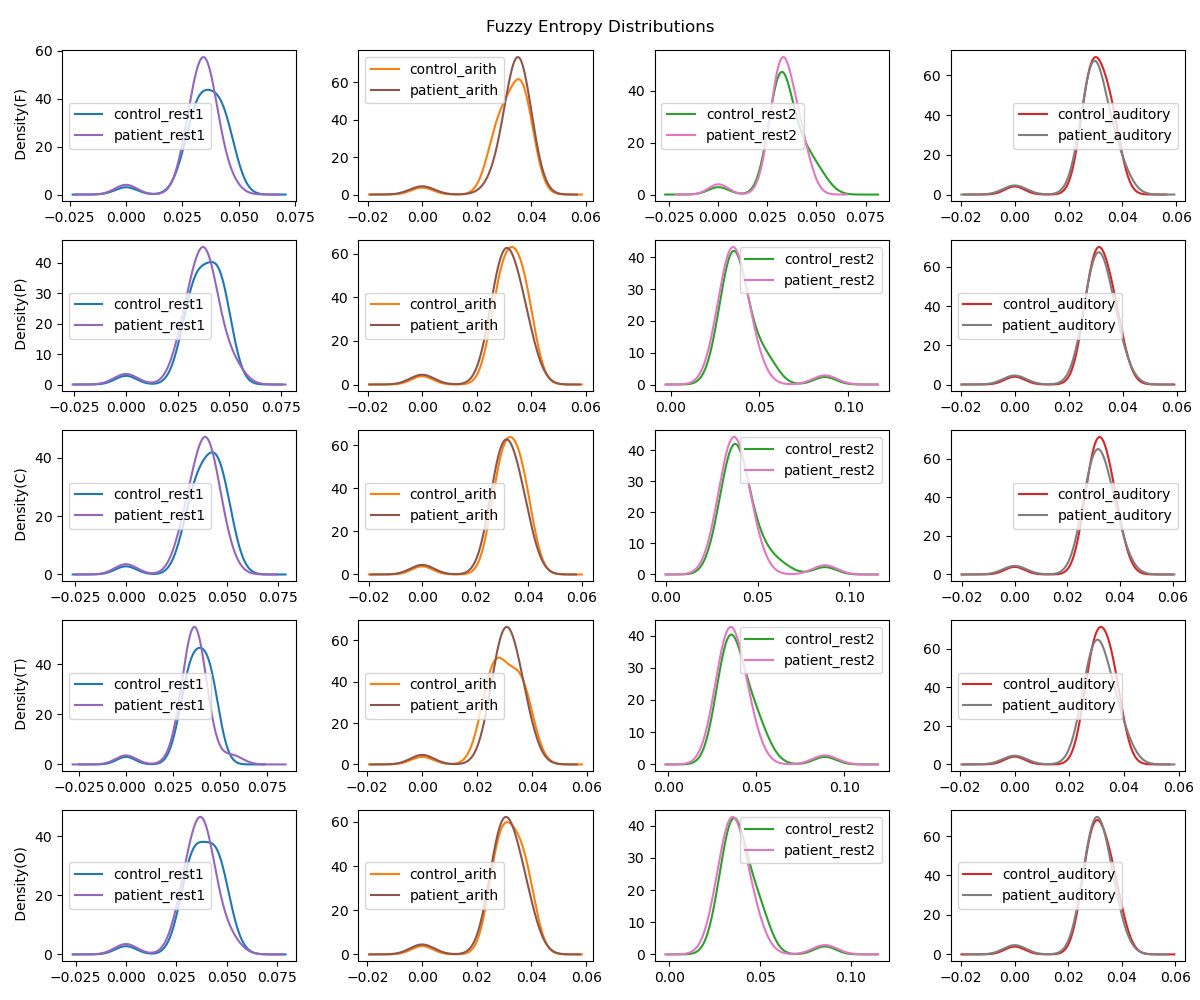
\includegraphics[width=16cm]{../../../data_analysis_results/FuzzEnt/corticalRegions_DAQphase_distributions.png}
  \caption{Fuzzy Entropy from controls}\label{fuzz_ent_distributions}
\end{figure}

\begin{figure}[H]
  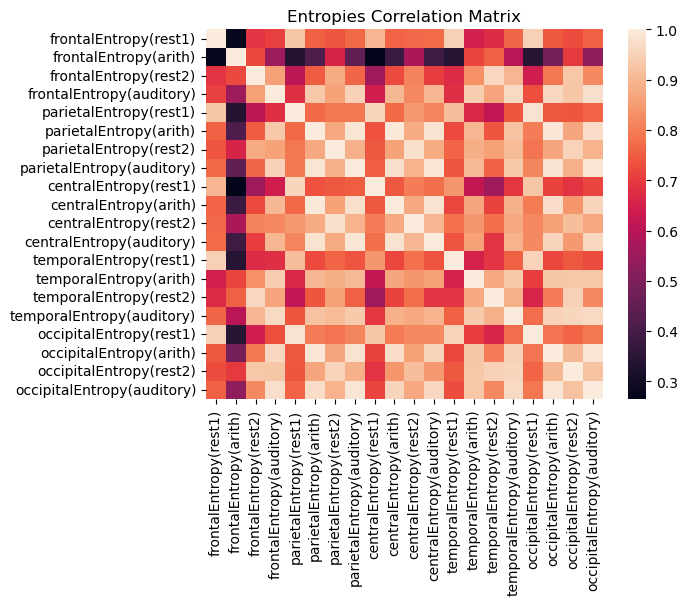
\includegraphics[width=16cm]{../../../data_analysis_results/FuzzEnt/entropies_corr_mat.png}
  \caption{Fuzzy-entropy values correlation smatrix}\label{fuzz_ent_corr_mat}
\end{figure}

\begin{figure}[H]
  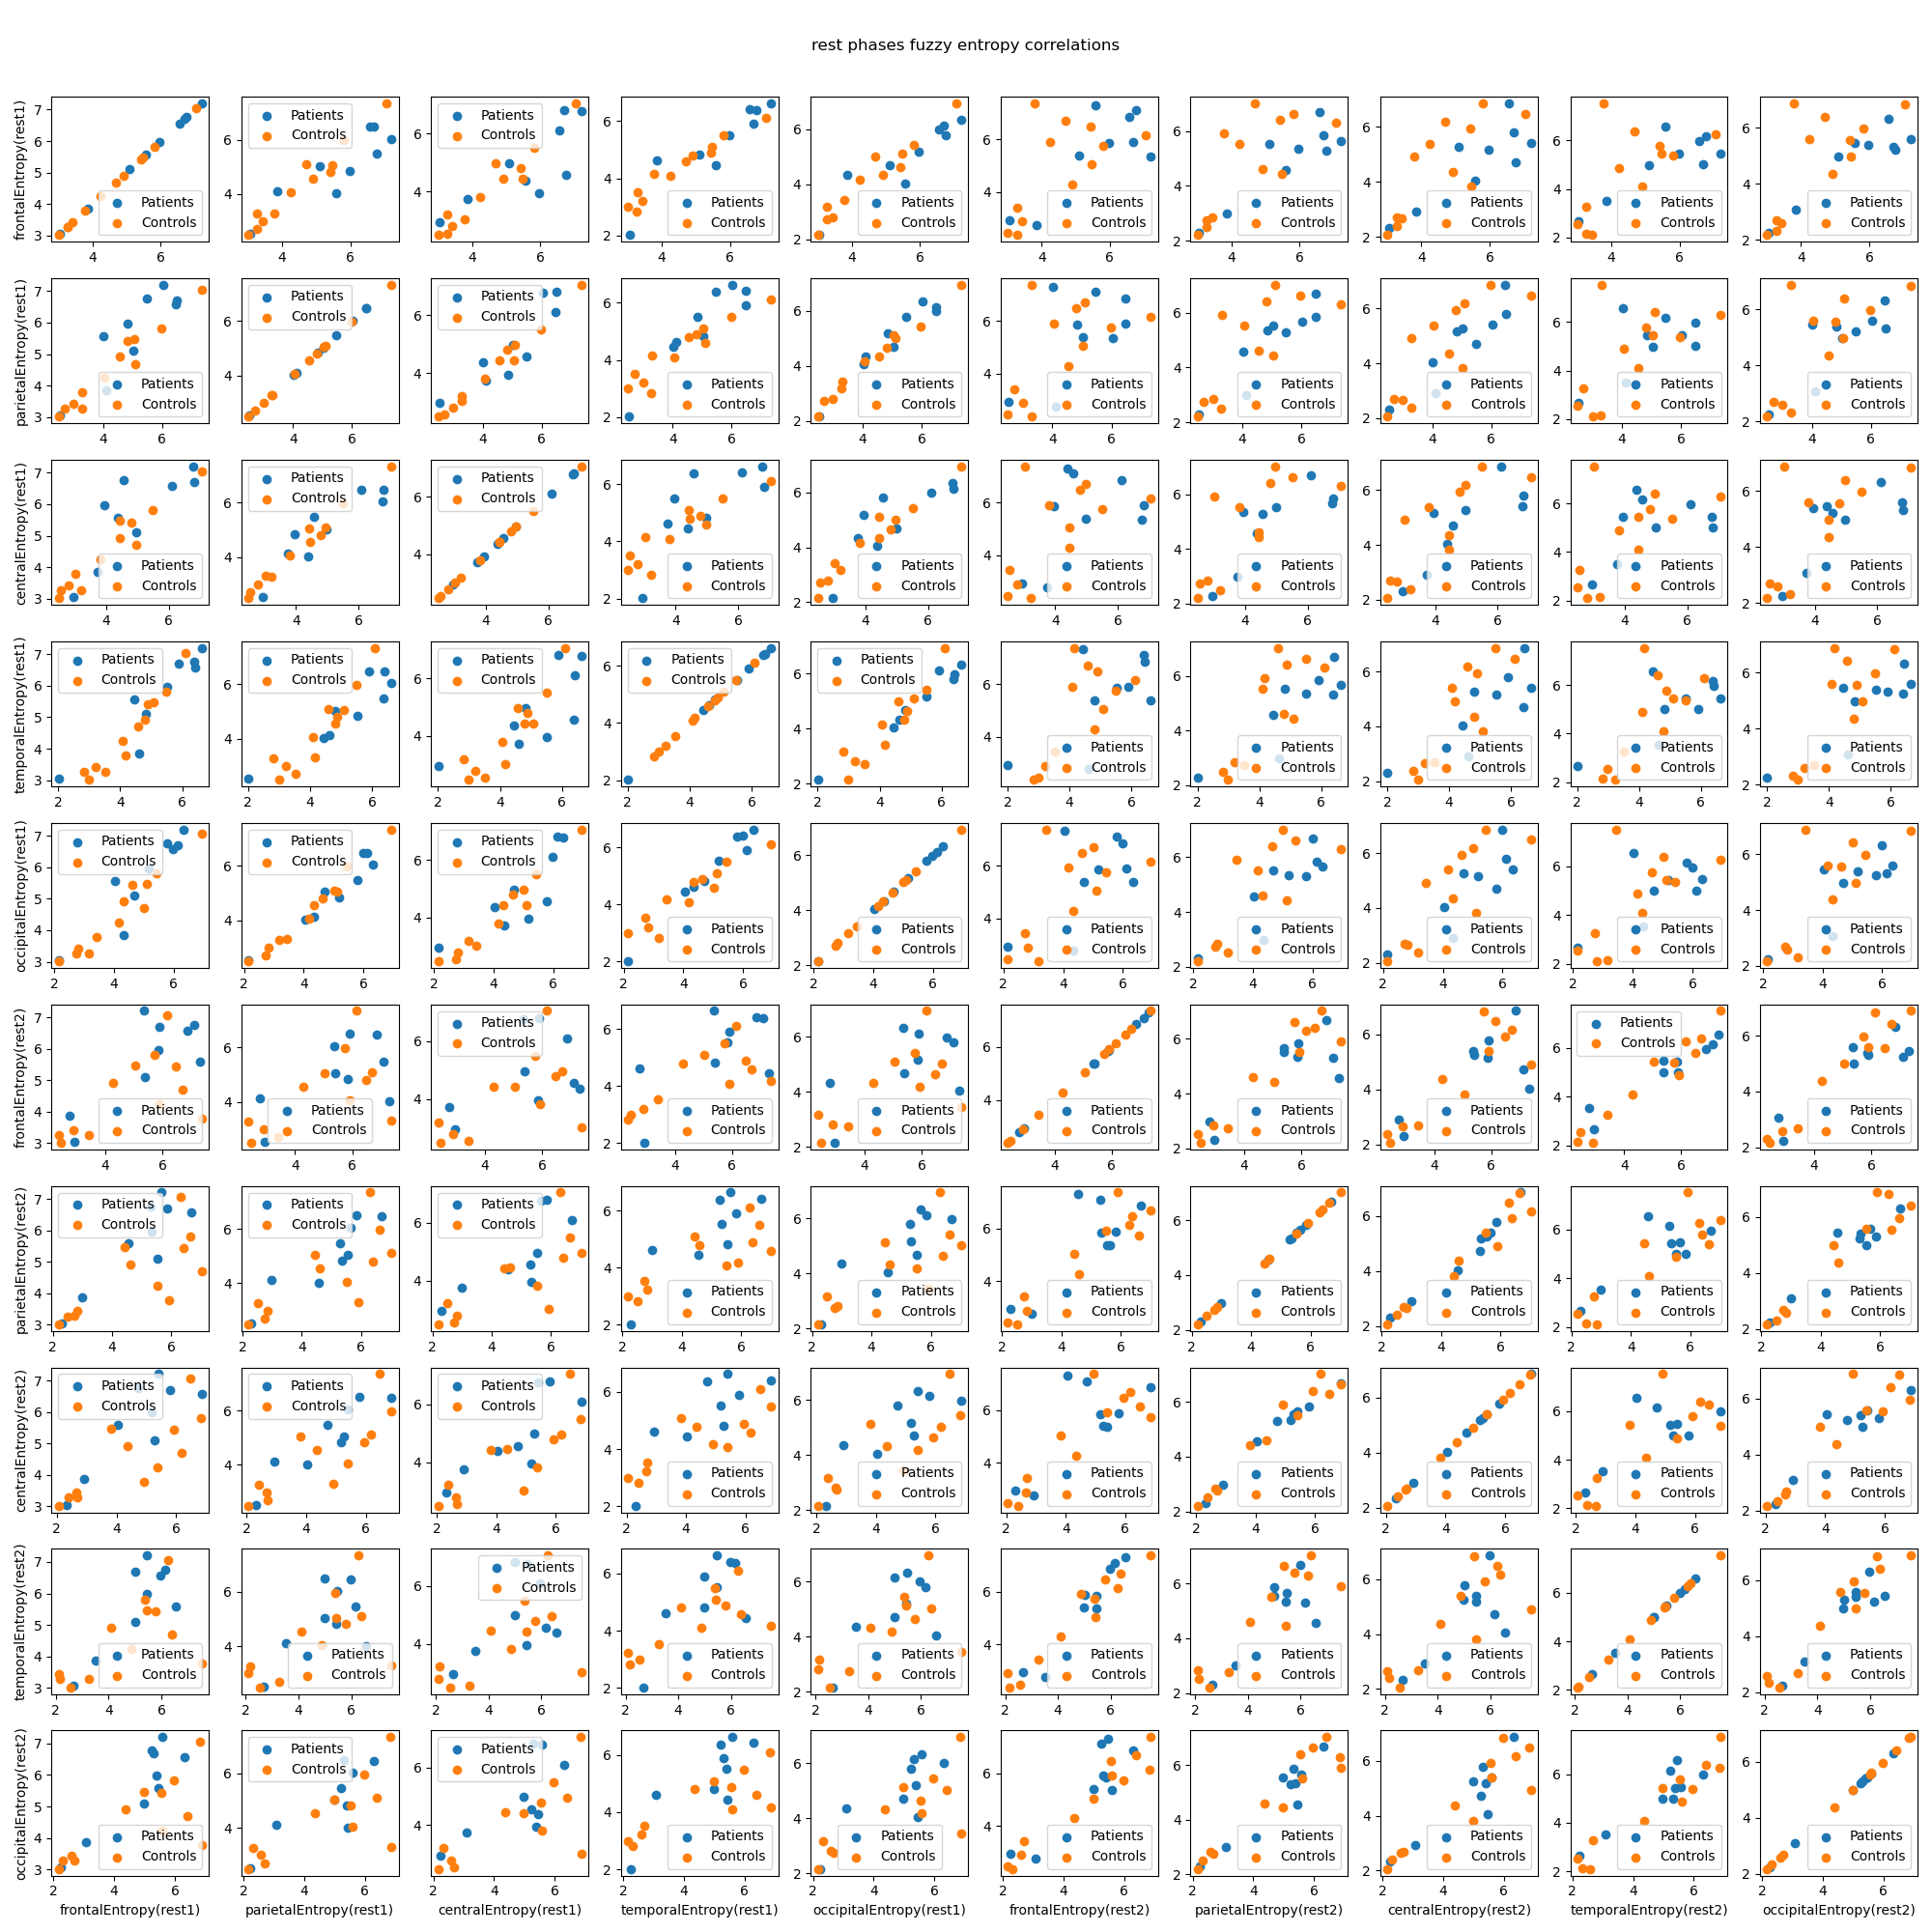
\includegraphics[width=16cm]{../../../data_analysis_results/FuzzEnt/rest_phases_corr.png}
  \caption{Rest Phases Fuzzy-entropy}\label{rest_fuzz}
\end{figure}
\begin{figure}[H]
  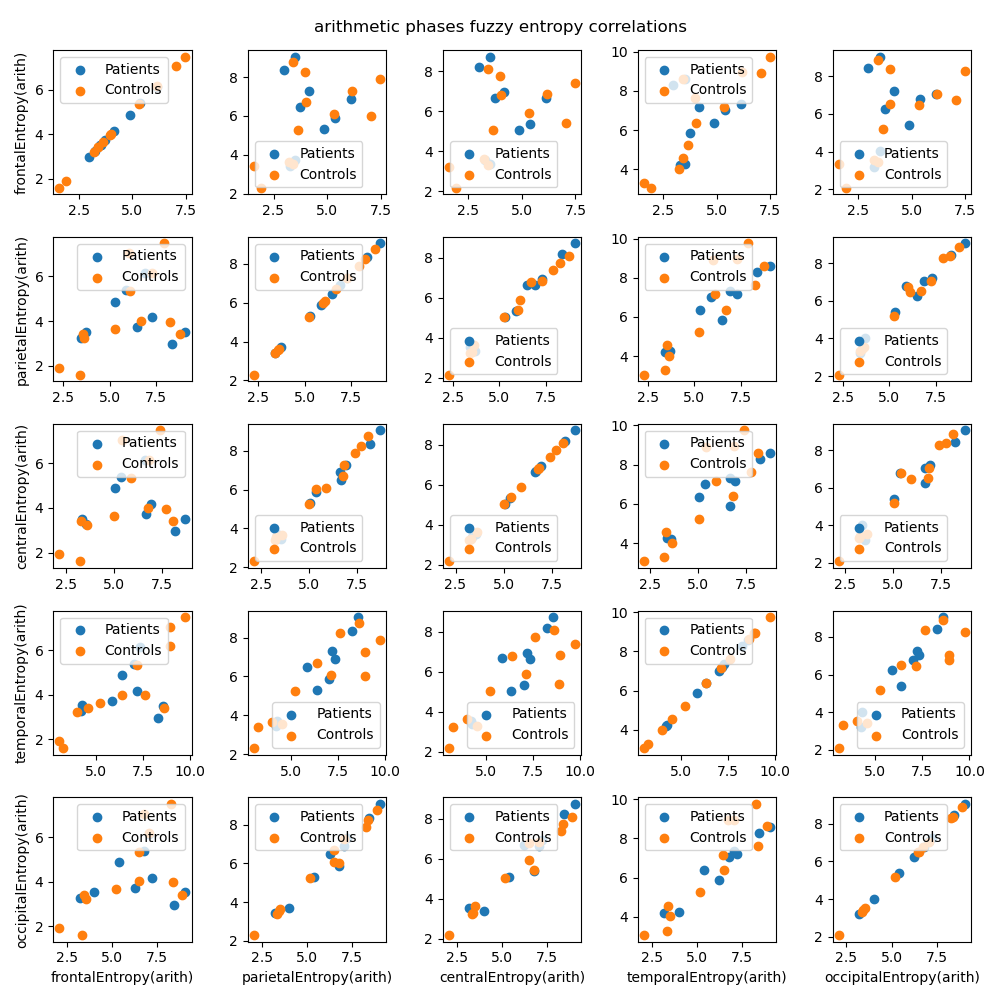
\includegraphics[width=16cm]{../../../data_analysis_results/FuzzEnt/arith_phases_corr.png}
  \caption{Arithmetic Phase Fuzzy-entropy}\label{arith_fuzz}
\end{figure}
\begin{figure}[H]
  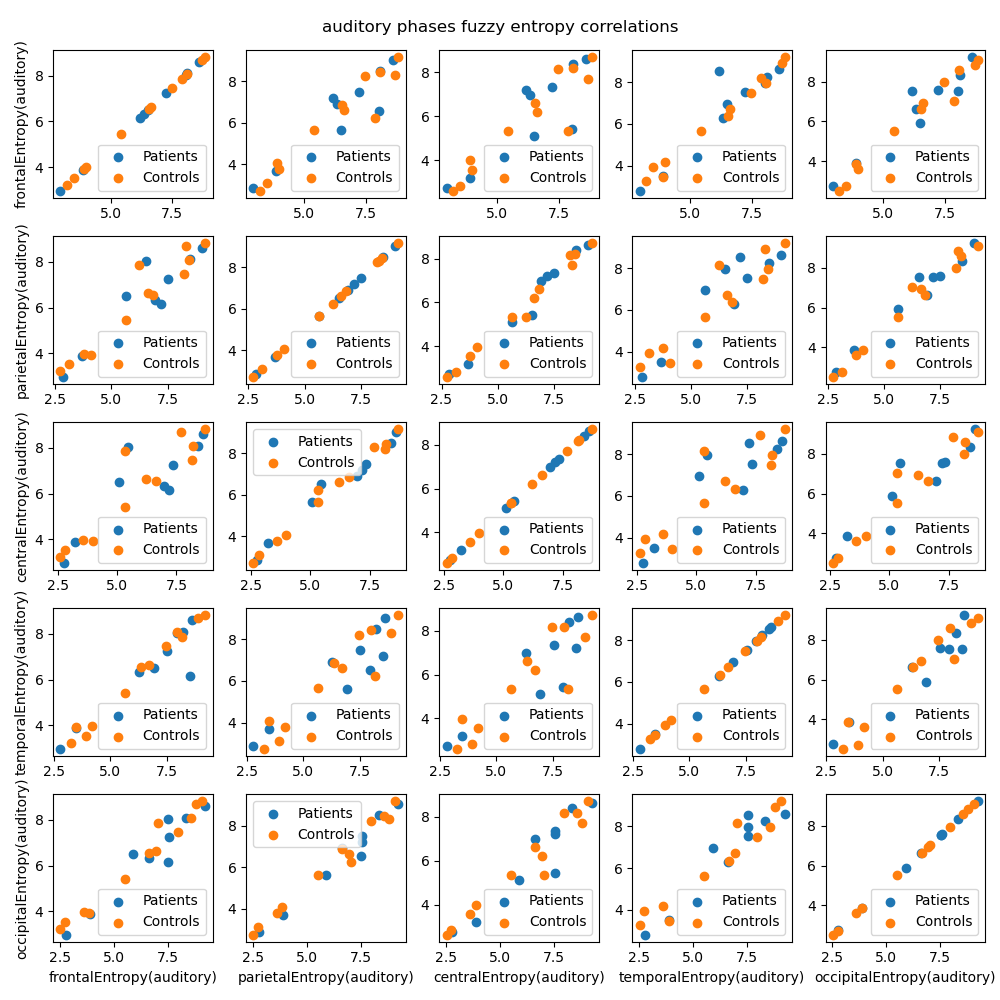
\includegraphics[width=16cm]{../../../data_analysis_results/FuzzEnt/auditory_phases_corr.png}
  \caption{Auditory Phase Fuzzy-entropy}\label{auditory_fuzz}
\end{figure}

\begin{figure}[H]
  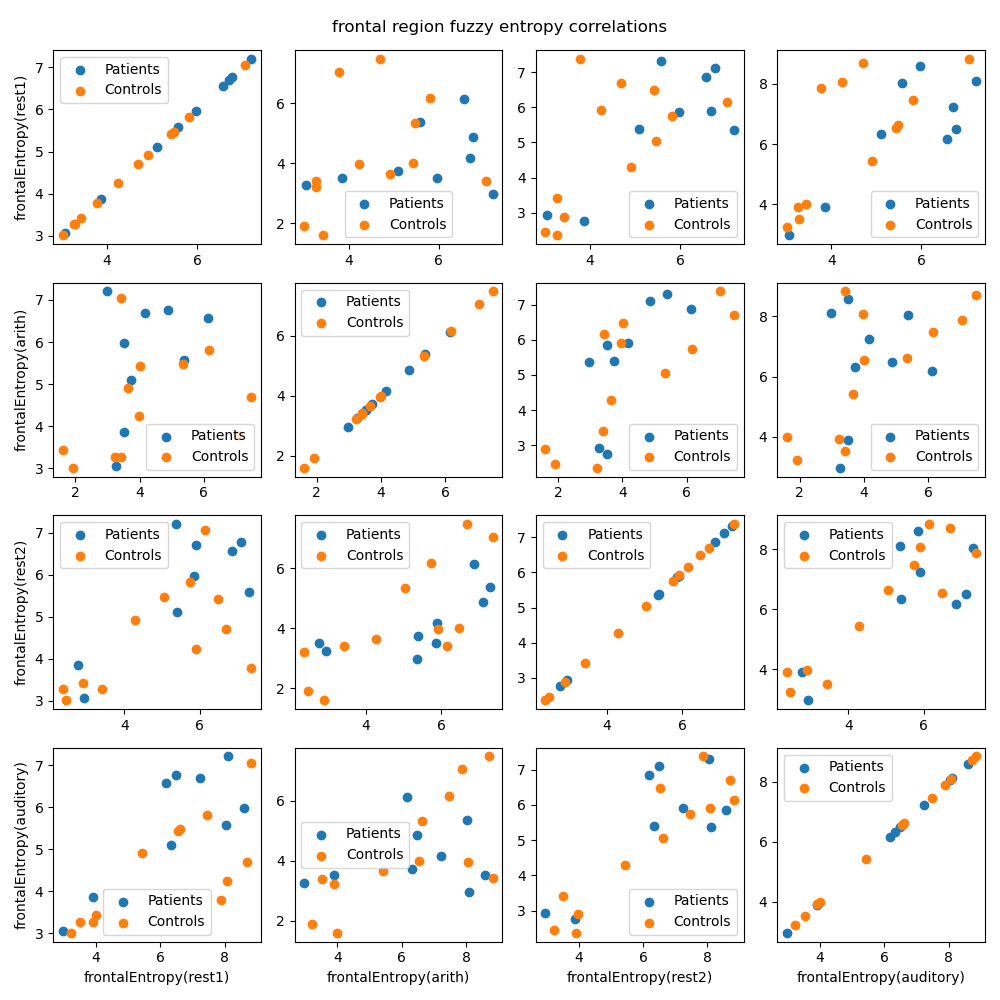
\includegraphics[width=16cm]{../../../data_analysis_results/FuzzEnt/frontal_region_corr.png}
  \caption{Frontal lobe Fuzzy-entropy}\label{frontal_fuzz}
\end{figure}
\begin{figure}[H]
  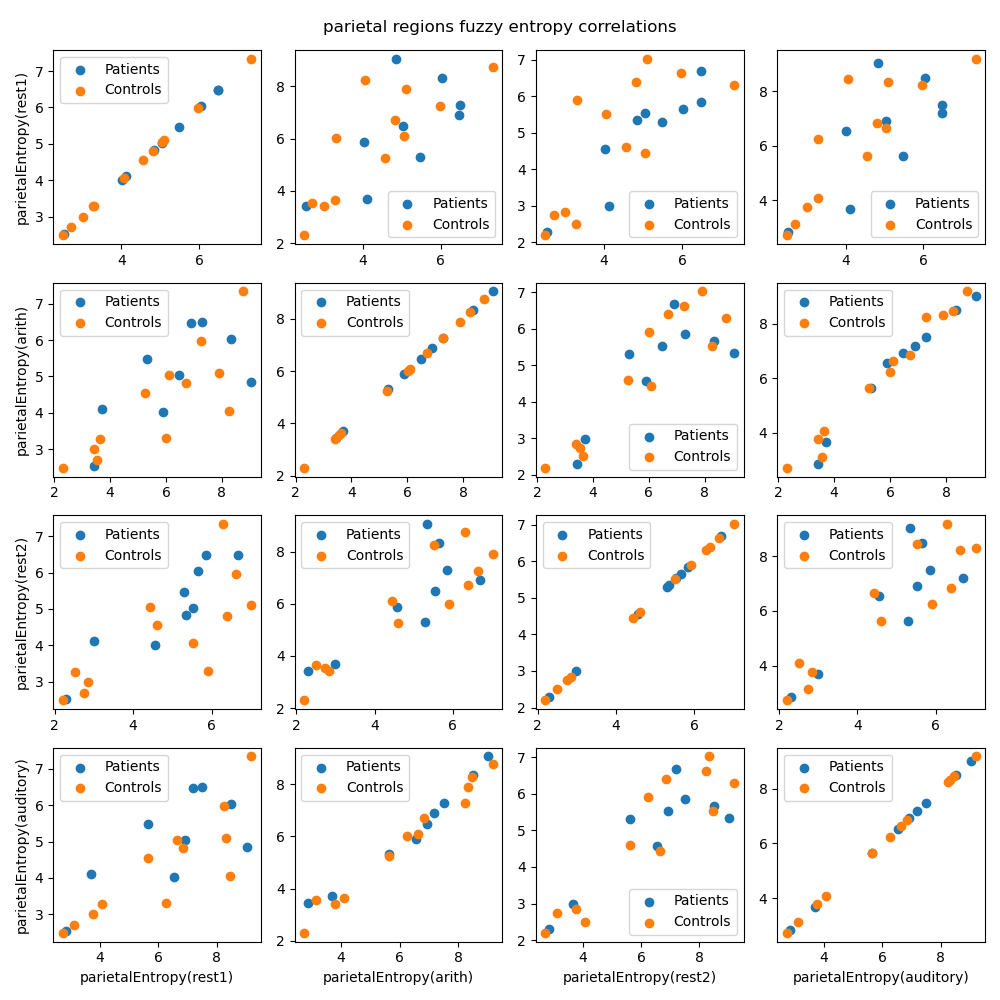
\includegraphics[width=16cm]{../../../data_analysis_results/FuzzEnt/parietal_region_corr.png}
  \caption{Parietal lobe Fuzzy-entropy}\label{parietal_fuzz}
\end{figure}
\begin{figure}[H]
  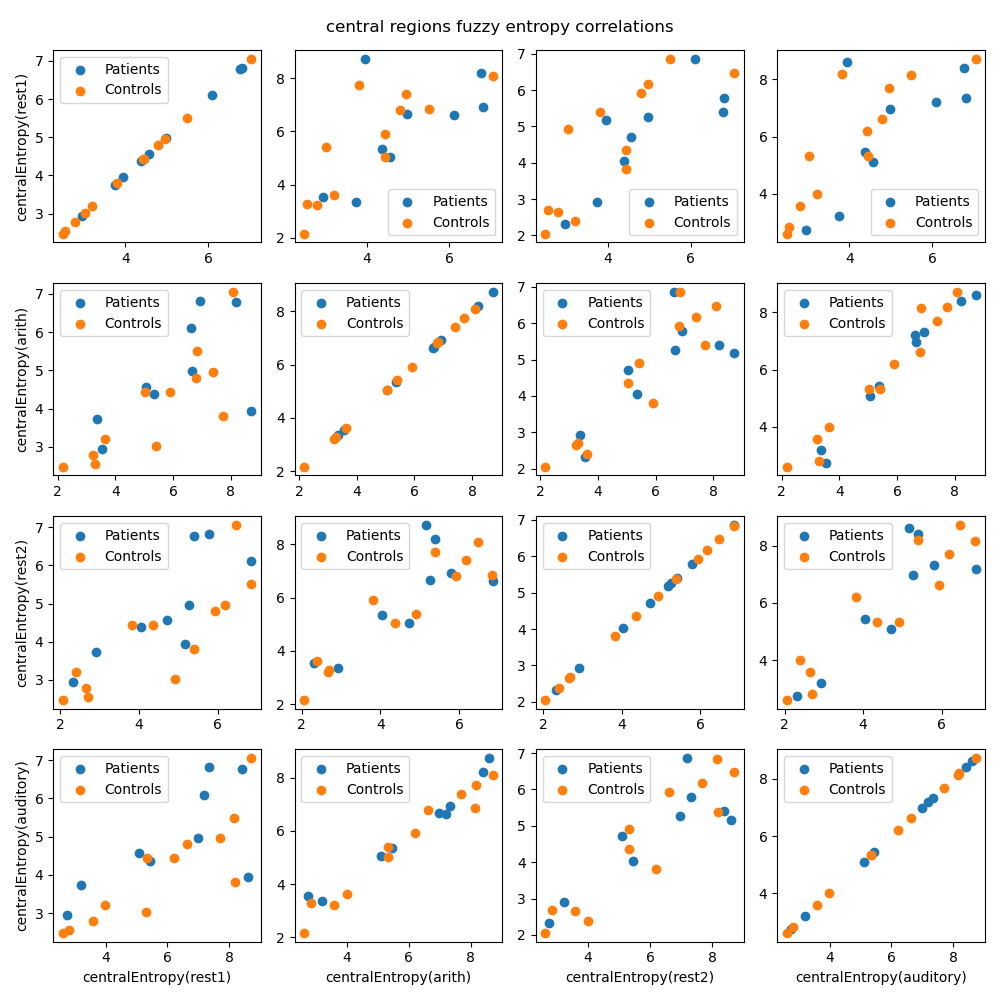
\includegraphics[width=16cm]{../../../data_analysis_results/FuzzEnt/central_region_corr.png}
  \caption{Central lobe Fuzzy-entropy}\label{central_fuzz}
\end{figure}
\begin{figure}[H]
  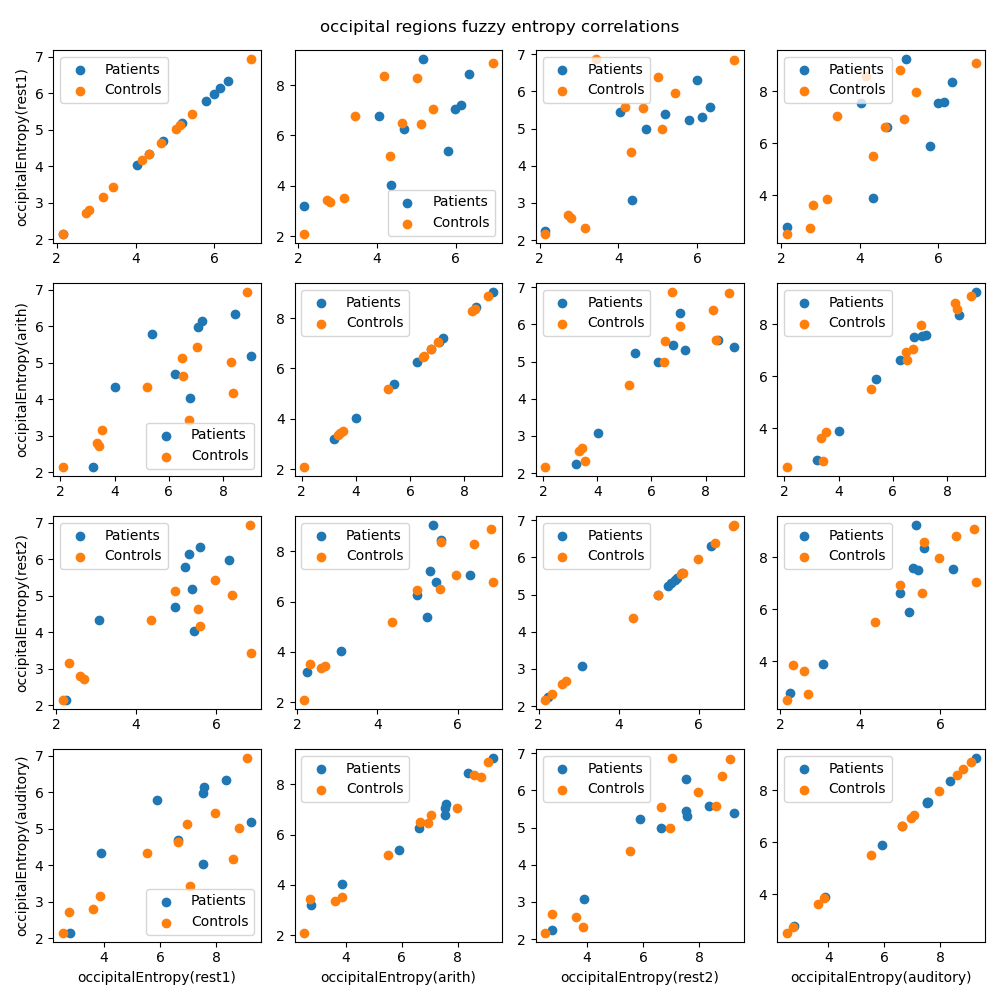
\includegraphics[width=16cm]{../../../data_analysis_results/FuzzEnt/occipital_region_corr.png}
  \caption{Occipital lobe Fuzzy-entropy}\label{occipital_fuzz}
\end{figure}
\begin{figure}[H]
  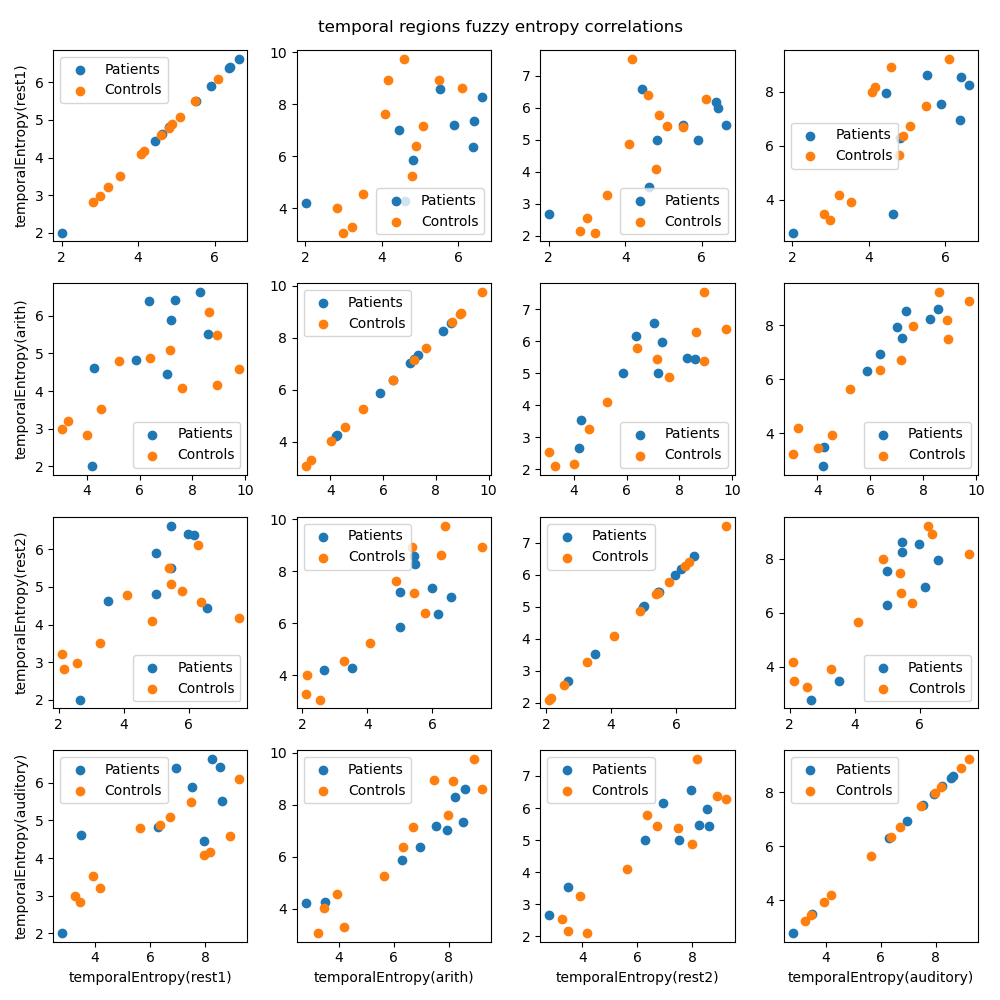
\includegraphics[width=16cm]{../../../data_analysis_results/FuzzEnt/temporal_region_corr.png}
  \caption{Temporal lobe Fuzzy-entropy}\label{temporal_fuzz}
\end{figure}

\end{document}
% \include{monthlly_report.acn}

%\journal{CSc 4110 Final Report}

%\title[journalExample]{Format for Project Reports}
\title{
  An update on the project: 
  \textbf{
      \textit{
        Development of an Automatic Instrument for Schizophrenia(SZ) Diagnosis
        }
      }, for the MCIP Innovation Prize 2022.
  }
% \author{
% Emmanuel OLATEJU \\
%     \begin{affiliation}
%       Supervised by Dr. K.P. Ayodele \\ 14/02/2023, \\
%       email: \mbox{kayodele@gmail.com, eoolateju@student.oauife.edu.ng}
%     \end{affiliation}
% }

\begin{document}
\maketitle

\section{Overview}
The purpose of this project is to design an instrument for early \gls{sz} diagnosis.
In designing the instrument, the following parts are to be developed:
\begin{itemize}
  \item An \gls{eeg} \gls{daq} system
  \item \gls{daq} user interface.
  \item Hand-clicker device for \gls{daq} process feedback from patient and clinicians.
  \item Machine/deep learning model.
  \item Soft instrument interacting with learnt model, \gls{daq} software, handheld 
  clicker, \gls{eeg} headbox and all developed parts.
  
\end{itemize}
The goal is to develop a medical turnkey device for \gls{sz} diagnosis having its own 
\gls{eeg} device and deeply embedded software. The long-term goal is for this turnkey device 
and its software to be built around the OpenBCI \gls{eeg} kit. The OpenBCI is chosen as
minimal number of electrode sites needed for \gls{sz} diagnosis may be identified and thus 
an \gls{eeg} kit that allows for flexibility of electrodes to be used is needed. This will 
mitigate the cost of the device making it more accessible. In the short term, the contec 
\gls{eeg} headbox is being used in identifying the best electrode sites.

The contec \gls{eeg} headbox is being used in place of the OpenBCI headbox temporarily 
for generation of the \gls{eeg} signals.
In order to fetch \gls{eeg} signals from the headbox, a piece of software that interacts 
with the contec's firmware has been developed. This piece of software has been incorporated 
with a user interface developed that makes \gls{daq} sessions interactive for both 
subjects and clinicians. The user interface and firmware interacting code together make 
up the Generis software presented in the first report.

In order to make \gls{daq} sessions more interactive, a handheld clicker is being developed 
to help patients and clinicians give feedback to the Generis software. Annotations can be 
somewhat a tough technical task and in certain cases becomes an headache for non-technical 
users. Once annotation messagess are configured into this clicker device, adding annotations 
will be redced to a task of simply clicking color coded buttons. This piece of hardware 
will also improve processing of signals as time during \gls{daq} of noise causing actions can be 
annotated and also times of subject inactivity or inert state to \gls{daq}. The handheld clicker 
is able to communicate with the Generis software through UART to USB communication.

In order to have an instrument of high accuracy and to solve the problem of \gls{sz} diagnosis 
being based on psychiatric nosology, the instrument(model) must be calibrated to seperate 
\glspl{szPtnt} from \glspl{hc}. This is being done using machine-learning and/or 
deep-learning methods and signal-processing algorithms to extract information relevant to 
\gls{sz} measurement and to improve discriminability.

The final instrument that integrates all of the designed parts is to be devloped upon 
completion of the handheld clicker and complete development of model to be used in 
measuring the extent of \gls{sz} disorder and classification of subjects. The structure 
of the final instrument is shown in the diagram below.
\begin{figure}[H]
  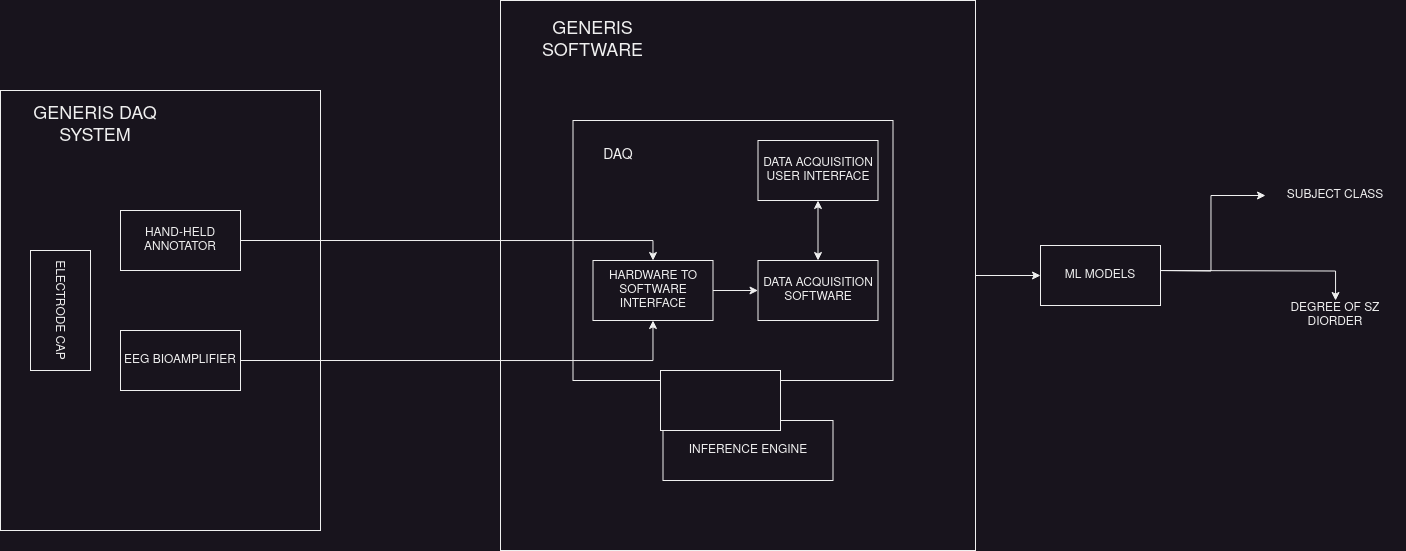
\includegraphics[width=16cm]{../../../images/technical/instrument.drawio.png}
  \caption{\gls{sz} diagnosis instrument}\label{instrument}
\end{figure}


\section{Handheld clicker}
The handheld clicker design is based on an arduino nano which applies the output of four 
tact switches as inputs to four vectored interrupts on the nano development board. The 
exact labels of these inputs has not been assigned as a study of the erogonomics of 
conventions employed in other devices of this kind and how best conventions are adapted and 
modified for the use case of this project is being studied. 

The current design of the handheld clicker(annotator) is the second iteration and is referred 
to as HC-v0.2. 
The circuit diagram of the handheld clicker is given in figure \ref{clicker_circuit}.
The flowchart describing the algorithm of this device is shown in figure \ref{clicker_flowchart}. 
The front and top images of the hand-clicker-v0.2 are shown in figures \ref{clicker} and 
\ref{top_view_of_clicker}.
\begin{figure}[H]
  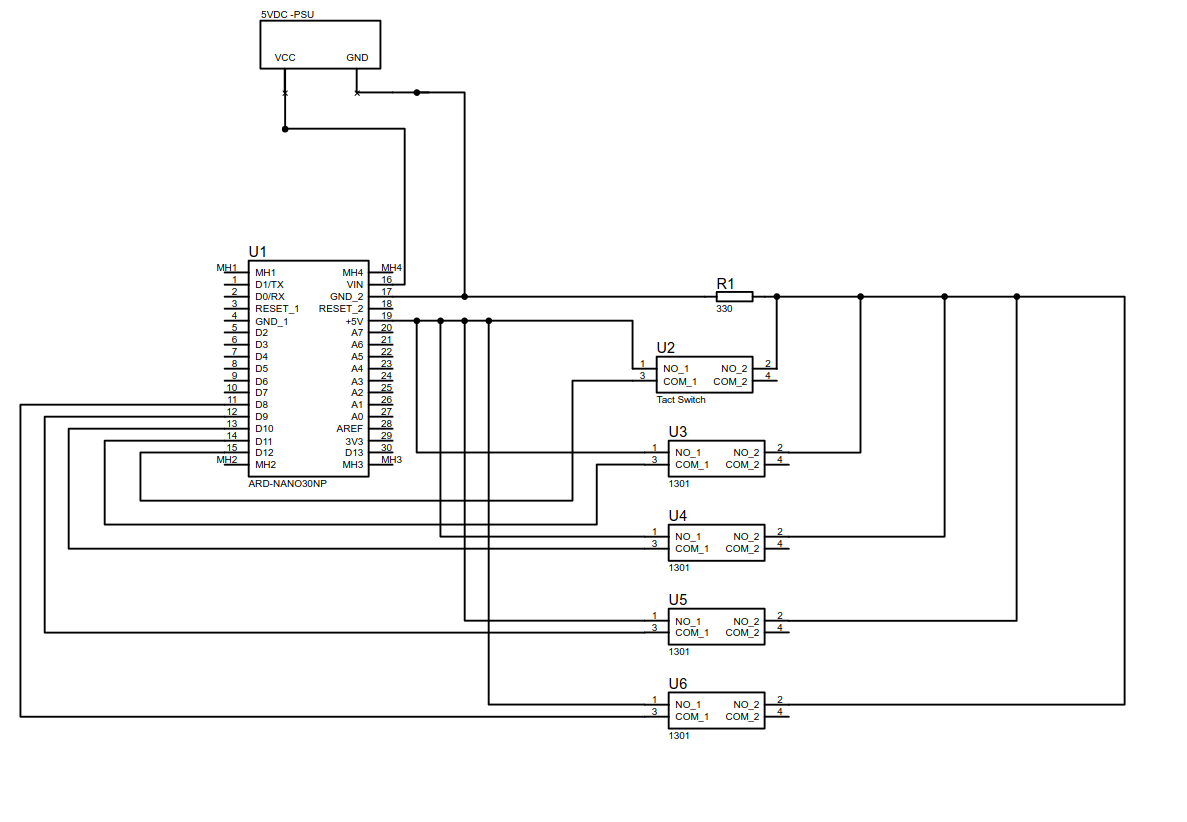
\includegraphics[width=16cm]{../../../hardware/handheld_clicker/circuit_image.png}
  \caption{handheld clicker circuit}\label{clicker_circuit}
\end{figure}
\begin{figure}[H]
  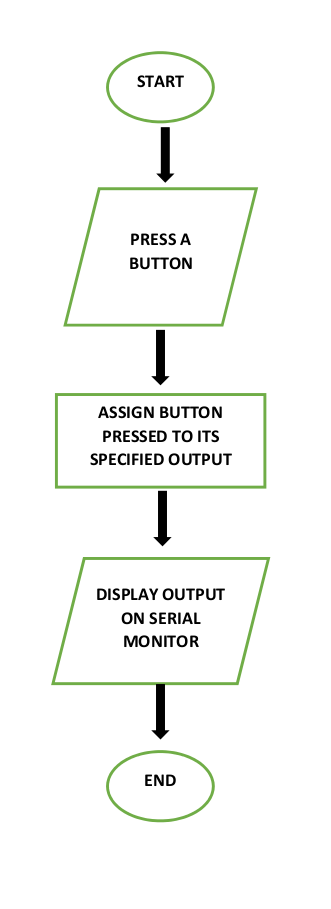
\includegraphics[height=16cm,width=10cm]{../../../hardware/handheld_clicker/flowchart.png}
  \caption{Flowchart algorithm of clicker}\label{clicker_flowchart}
\end{figure}
\begin{figure}[H]
  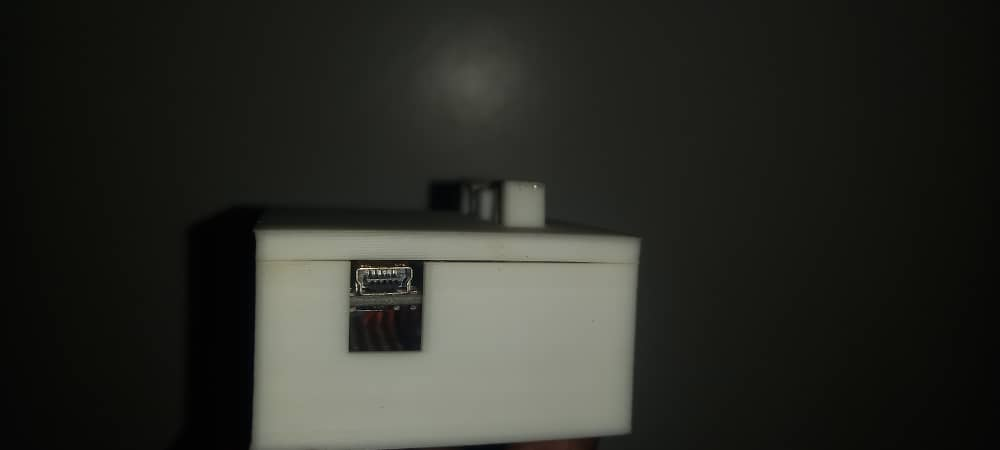
\includegraphics[width=16cm]{../../../hardware/handheld_clicker/front.jpeg}
  \caption{Front view of clicker}\label{clicker}
\end{figure}
\begin{figure}[H]
  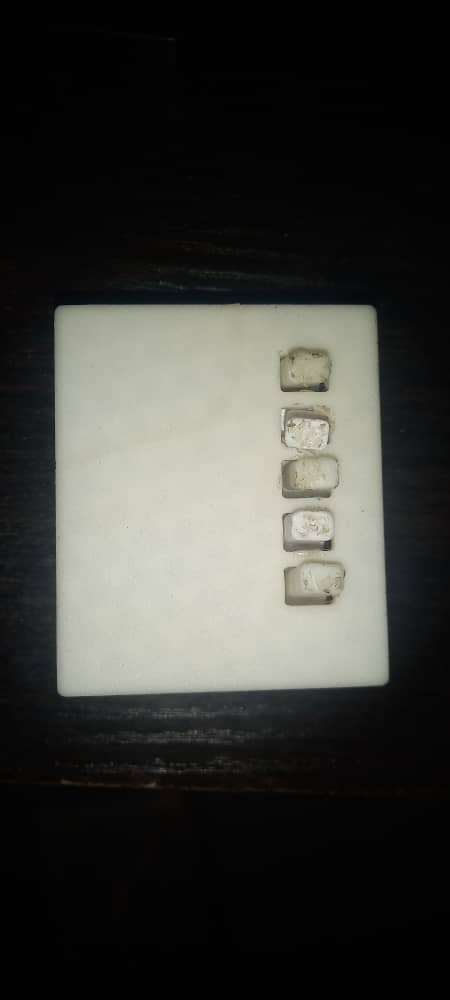
\includegraphics[,height=10cm,width=8cm]{../../../hardware/handheld_clicker/top.jpeg}
  \caption{Top view of clicker}\label{top_view_of_clicker}
\end{figure}


\section{Model Development (Feature-extraction, Data-analysis)}
\subsection{Feature Extraction}
March's report presented the fuzzy entropy features extracted from cortical
regions during phases of \gls{daq} and also the refined \gls{mmn} plots which 
made the \gls{mmn} waveform more evident. Relevant changes made to features 
extraction highlighted in marchs's report includes:
\begin{itemize}
  \item Recomputing the \gls{mmn} waveforms
  \item Spatial dimension augmentation with gaussian noise during computation of fuzzy-entropy
  \item Development of custom fuzzy-entropy library
\end{itemize}
The following was proposed as the next set of action points:
\begin{itemize}
  \item The continued improvement of fuzzy-entropy library to work with multivariate \\
  time-series(2D data)
  \item comparing performance of the fuzzy-entropy features from sourced library to \\
  that of the personally developed library
  \item Computing the auditory steady state features
\end{itemize}
A slight detour was made from these proposed action points for the month of april. 
Analysis of the extracted features for levels of dicriminability was carried out 
to understand how to improve the features extraction methods. The analysis shows 
a significant level of discrimination in the \gls{mmn} features, less in the 
fuzzy-entropy features, though the correlation patterns of the fuzzy-entropy features 
suggest they might carry information on extent of \gls{sz} disorder.

\gls{mmn} features have been extracted from the scaled \gls{mmn} waveforms. The 
\gls{mmn} features were computed as the mean of the \gls{mmn} waveforms within 
the time-frames 0-100ms, 100-200ms, 200-300ms, 300-400ms, 400-450ms.

Formerly implemented montage plot algorithm was improved upon to reduce 
time-complexity so as to make data visualization and analysis easier to obtain 
intuitive information from.

\subsection{Data Analysis/Visualization}\label{data_analyis}
 Analysis of the extracted features was done to establish the quality of discriminative 
 and quantitative information contained in the extracted features. The method of 
 Visualization of some of these features changed to make analysis easy.
 The results of the analysis are given in section \ref{figures}. Visualization methods 
 and analysis carried out includes:
\begin{itemize}
  \item Comparing \gls{mmn} feature values for 1KHz duration deviant and 3KHz frequency deviant 
  between patient and controls across all electrodes and time windows.
  (Figures \ref{mmnvalue_0_100ms} - \ref{mmnvalue_400_450ms})
  \item Converting the \gls{mmn} values to montage plots for 1KHz duration deviant 
  and 3KHz frequency deviant for easier interpretation and analyzing montage evolution.
  (Figures \ref{control_1KHz_mmn_montage}-\ref{patient_3KHz_mmn_montage})
  \item Comparing distribution of computed fuzzy-entropy values of patients and controls 
  for each cortical region across all phases of \gls{daq}.
  (Figures \ref{fig:controlFuzzEnt}-\ref{fuzz_ent_distributions}) 
  \item Correlating fuzzy-entropy values from cortical regions across 
  all phases of \gls{daq}.(Figure \ref{fuzz_ent_corr_mat})
  \item Comparing entropies from all cortical regions for each phase of \gls{daq}.
  (Figures \ref{rest_fuzz}-\ref{auditory_fuzz})
  \item Comparing entropies from all phases of \gls{daq} for each cortical region.
  (figures \ref{frontal_fuzz}-\ref{temporal_fuzz})
\end{itemize} 

\section{Inference and Action Points}
\subsection{Inference}
From the analysis carried out, the \gls{mmn} features of both tone deviants show 
discriminative properties between the \gls{szPtnt} and \gls{hc} in localized head 
regions. The fuzzy-entropy features do not show discriminative abilities, but their 
correlation patterns indicate a linear relationship that might be a measure of degree 
of \gls{sz} disorder. Therefore we need to find methods that improve quality of extracted 
features and proceed with developing a learner model.

\subsection{Action Points}
Based on the inference drawn, the action points for the month of may is as follows:
\begin{itemize}
  \item Computing the auditory steady state features.
  \item Re-computing fuzzy-entropy features using other libraries and 
  comparing performance.
  \item Improve discriminability of features using spatial filters and dimensionality 
  reduction techniques.
  \item Compare performance of a custom mutilayer feedforward network and traditional 
  machine-learning algorithms for classification and estimation of measures of degree 
  of \gls{sz} disorder.
\end{itemize}

\section{Figures}\label{figures}

\begin{figure}[H]
  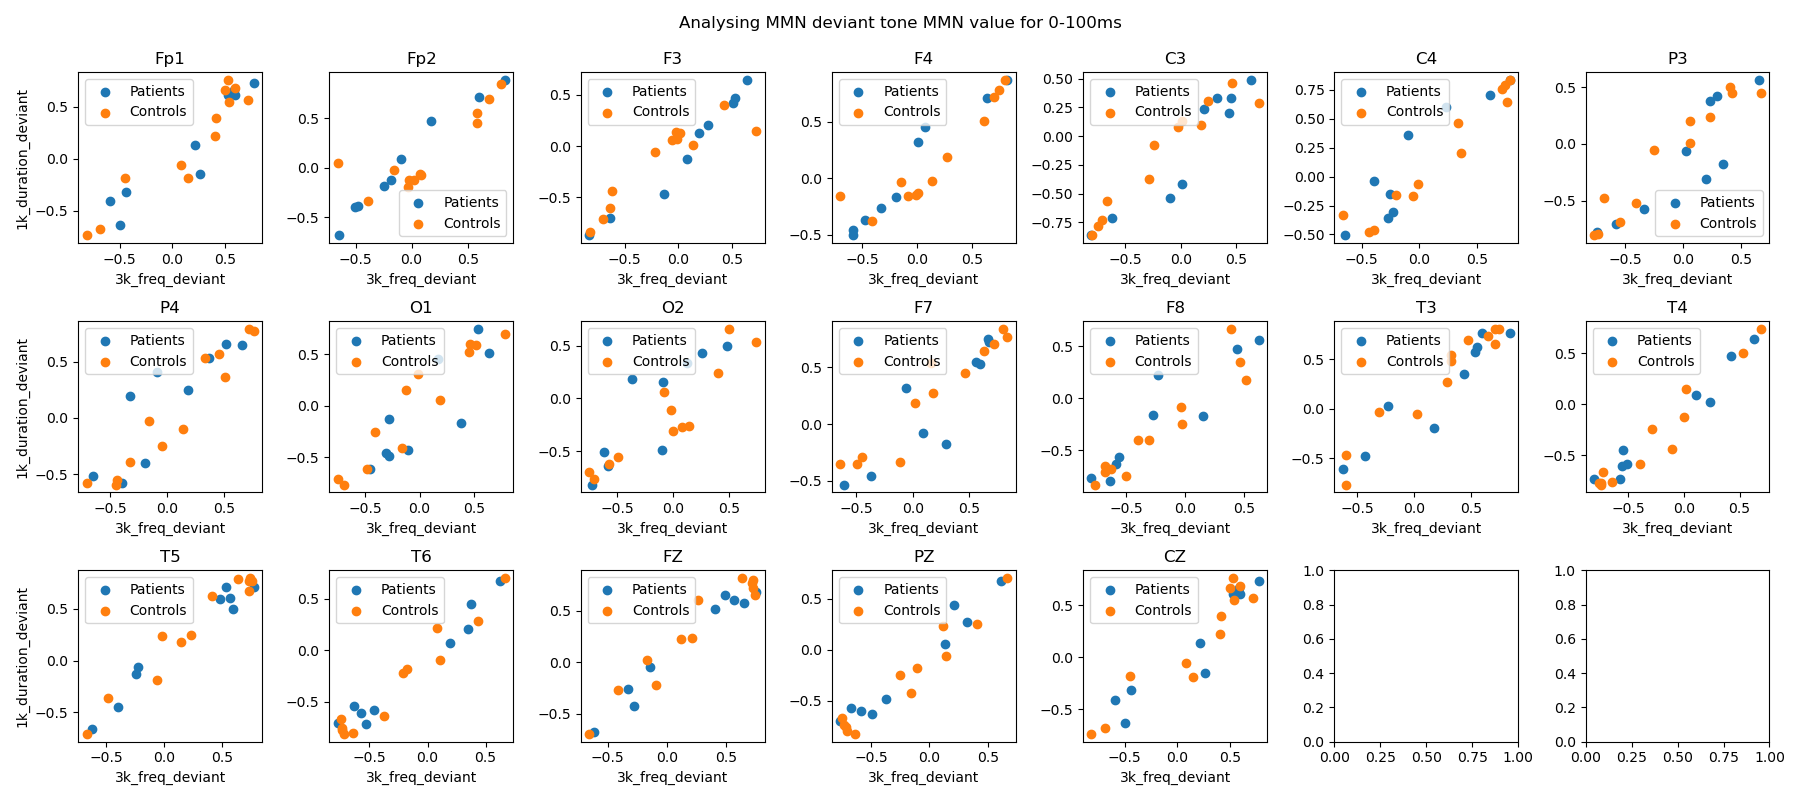
\includegraphics[width=16cm]{../../../data_analysis_results/MMN/features/deviant_tone_0.png}
  \caption{\gls{mmn} values from 0-100ms}\label{mmnvalue_0_100ms}
\end{figure}
\begin{figure}[H]
  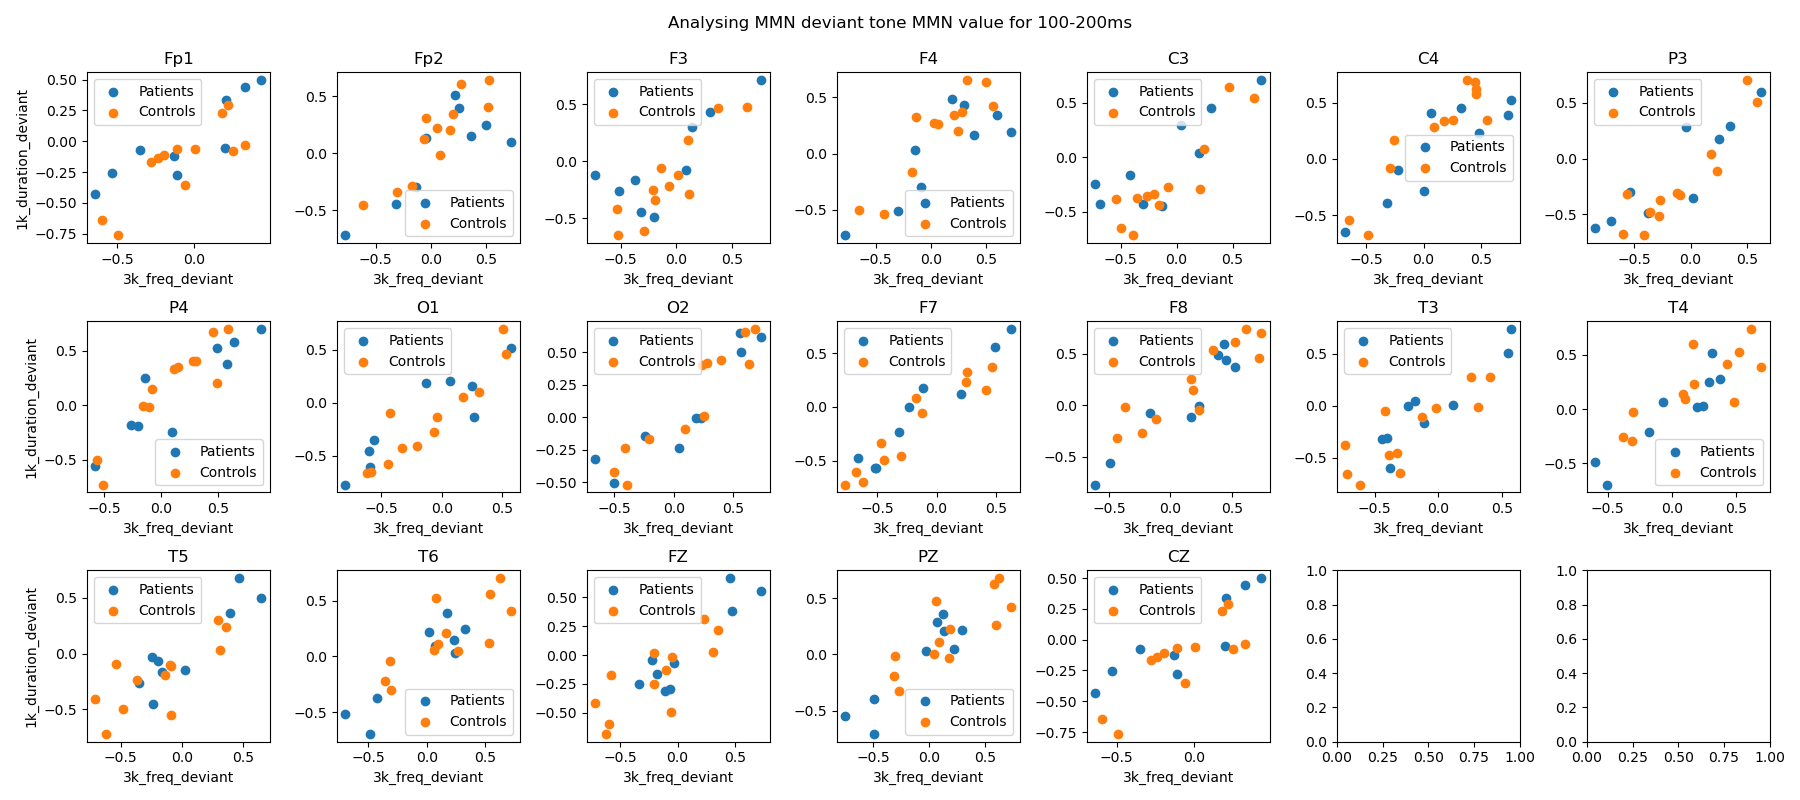
\includegraphics[width=16cm]{../../../data_analysis_results/MMN/features/deviant_tone_1.png}
  \caption{\gls{mmn} values from 100-200ms}\label{mmnvalue_100_200ms}
\end{figure}
\begin{figure}[H]
  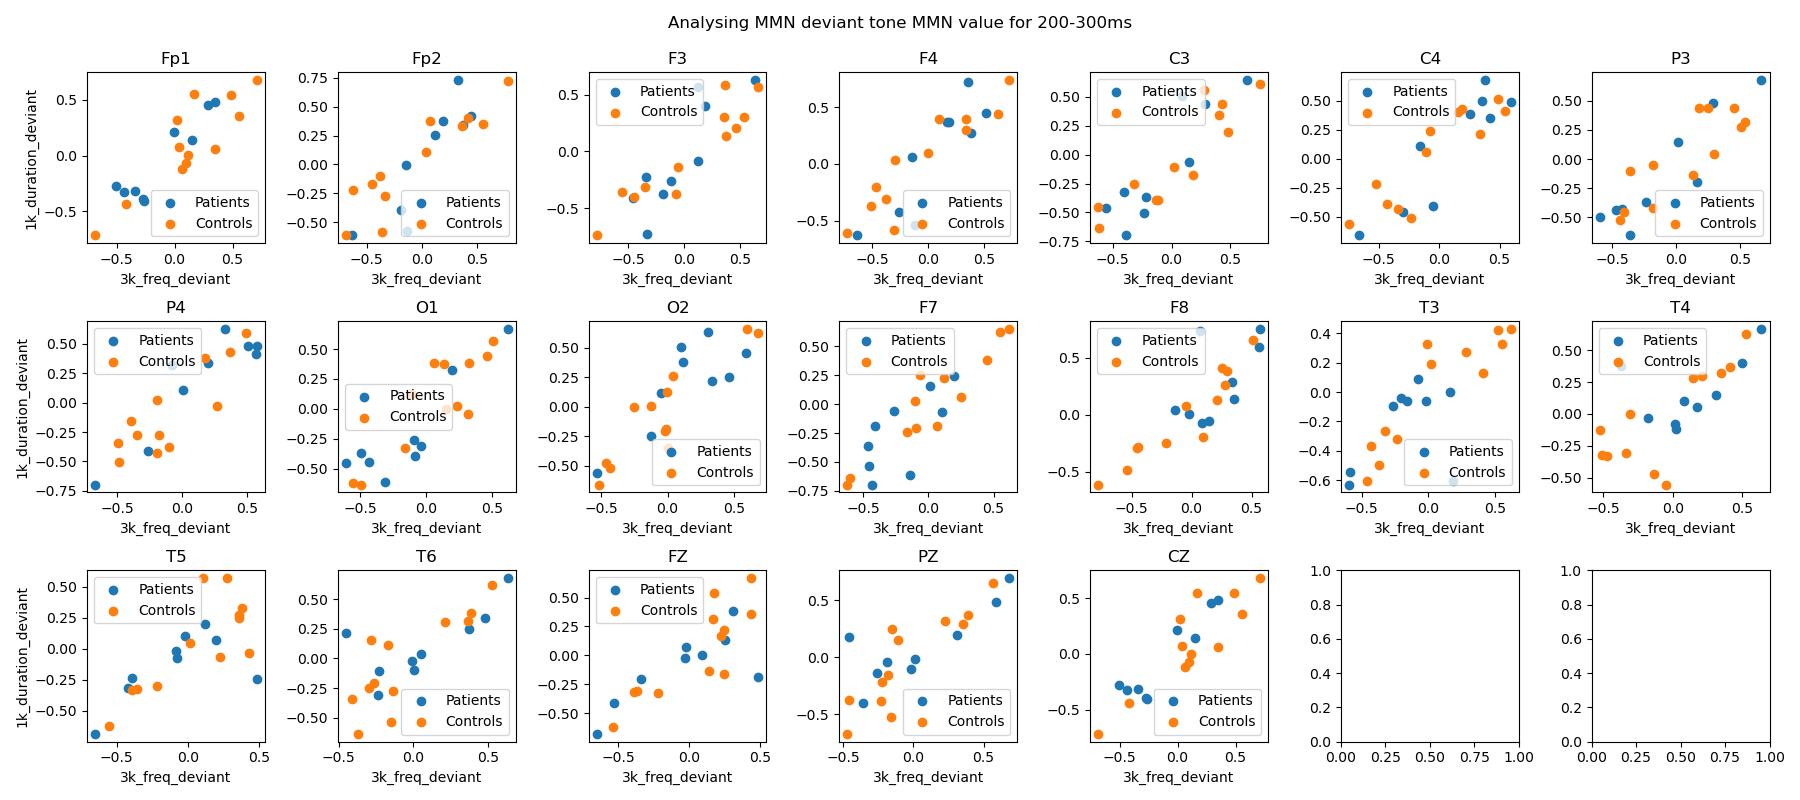
\includegraphics[width=16cm]{../../../data_analysis_results/MMN/features/deviant_tone_2.png}
  \caption{\gls{mmn} values from 200-300ms}\label{mmnvalue_200_300ms}
\end{figure}
\begin{figure}[H]
  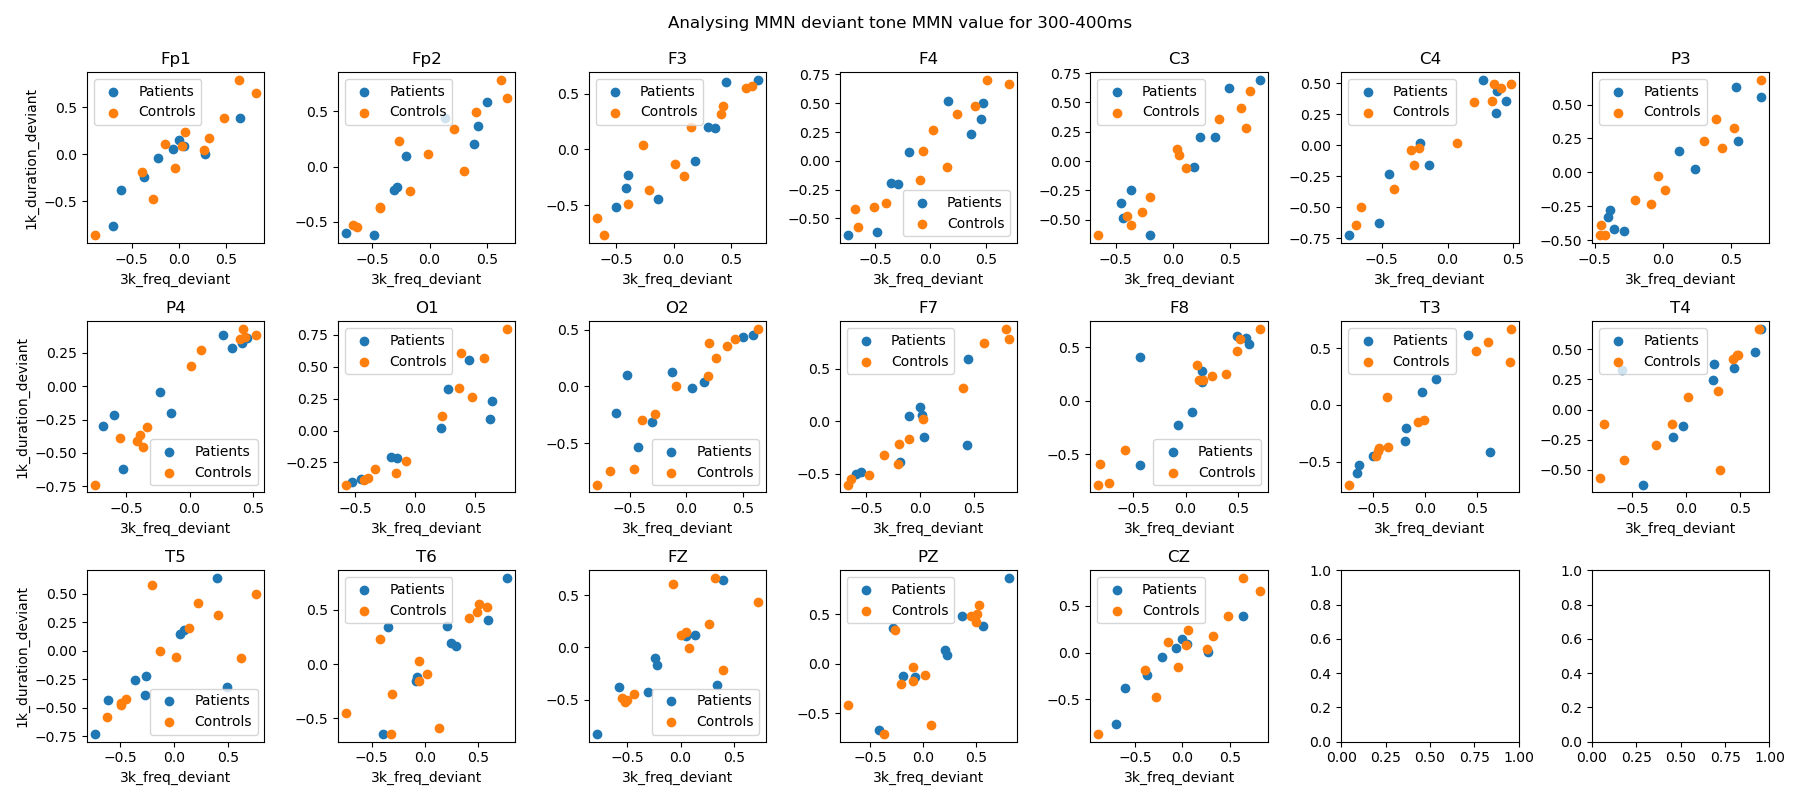
\includegraphics[width=16cm]{../../../data_analysis_results/MMN/features/deviant_tone_3.png}
  \caption{\gls{mmn} values from 300-400ms}\label{mmnvalue_300_400ms}
\end{figure}
\begin{figure}[H]
  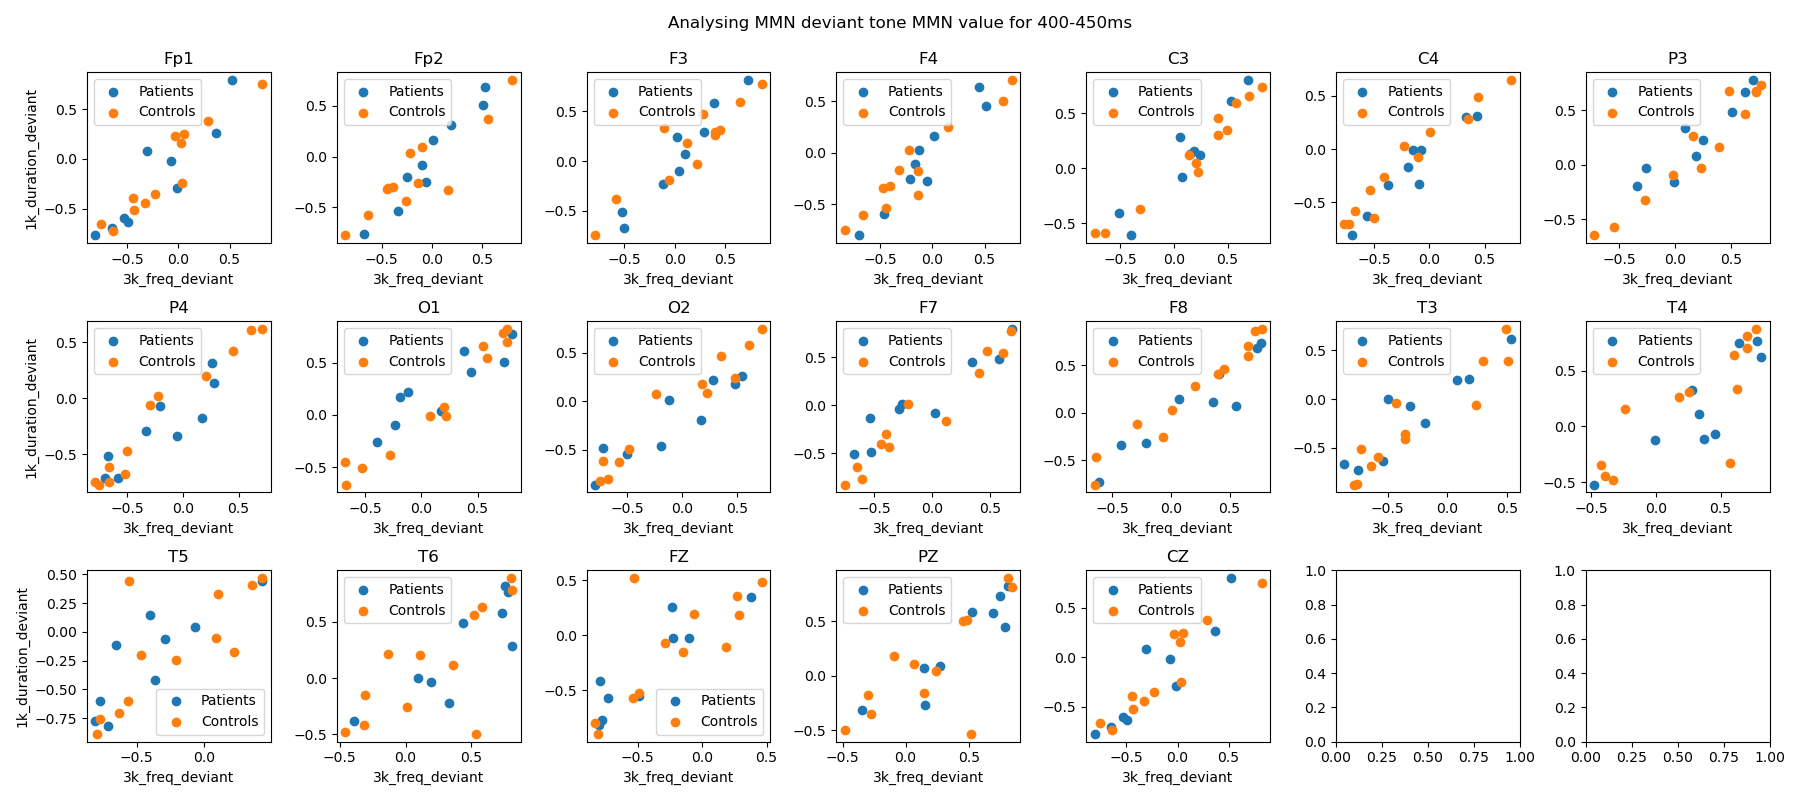
\includegraphics[width=16cm]{../../../data_analysis_results/MMN/features/deviant_tone_4.png}
  \caption{\gls{mmn} values from 400-450ms}\label{mmnvalue_400_450ms}
\end{figure}

\begin{figure}[H]
  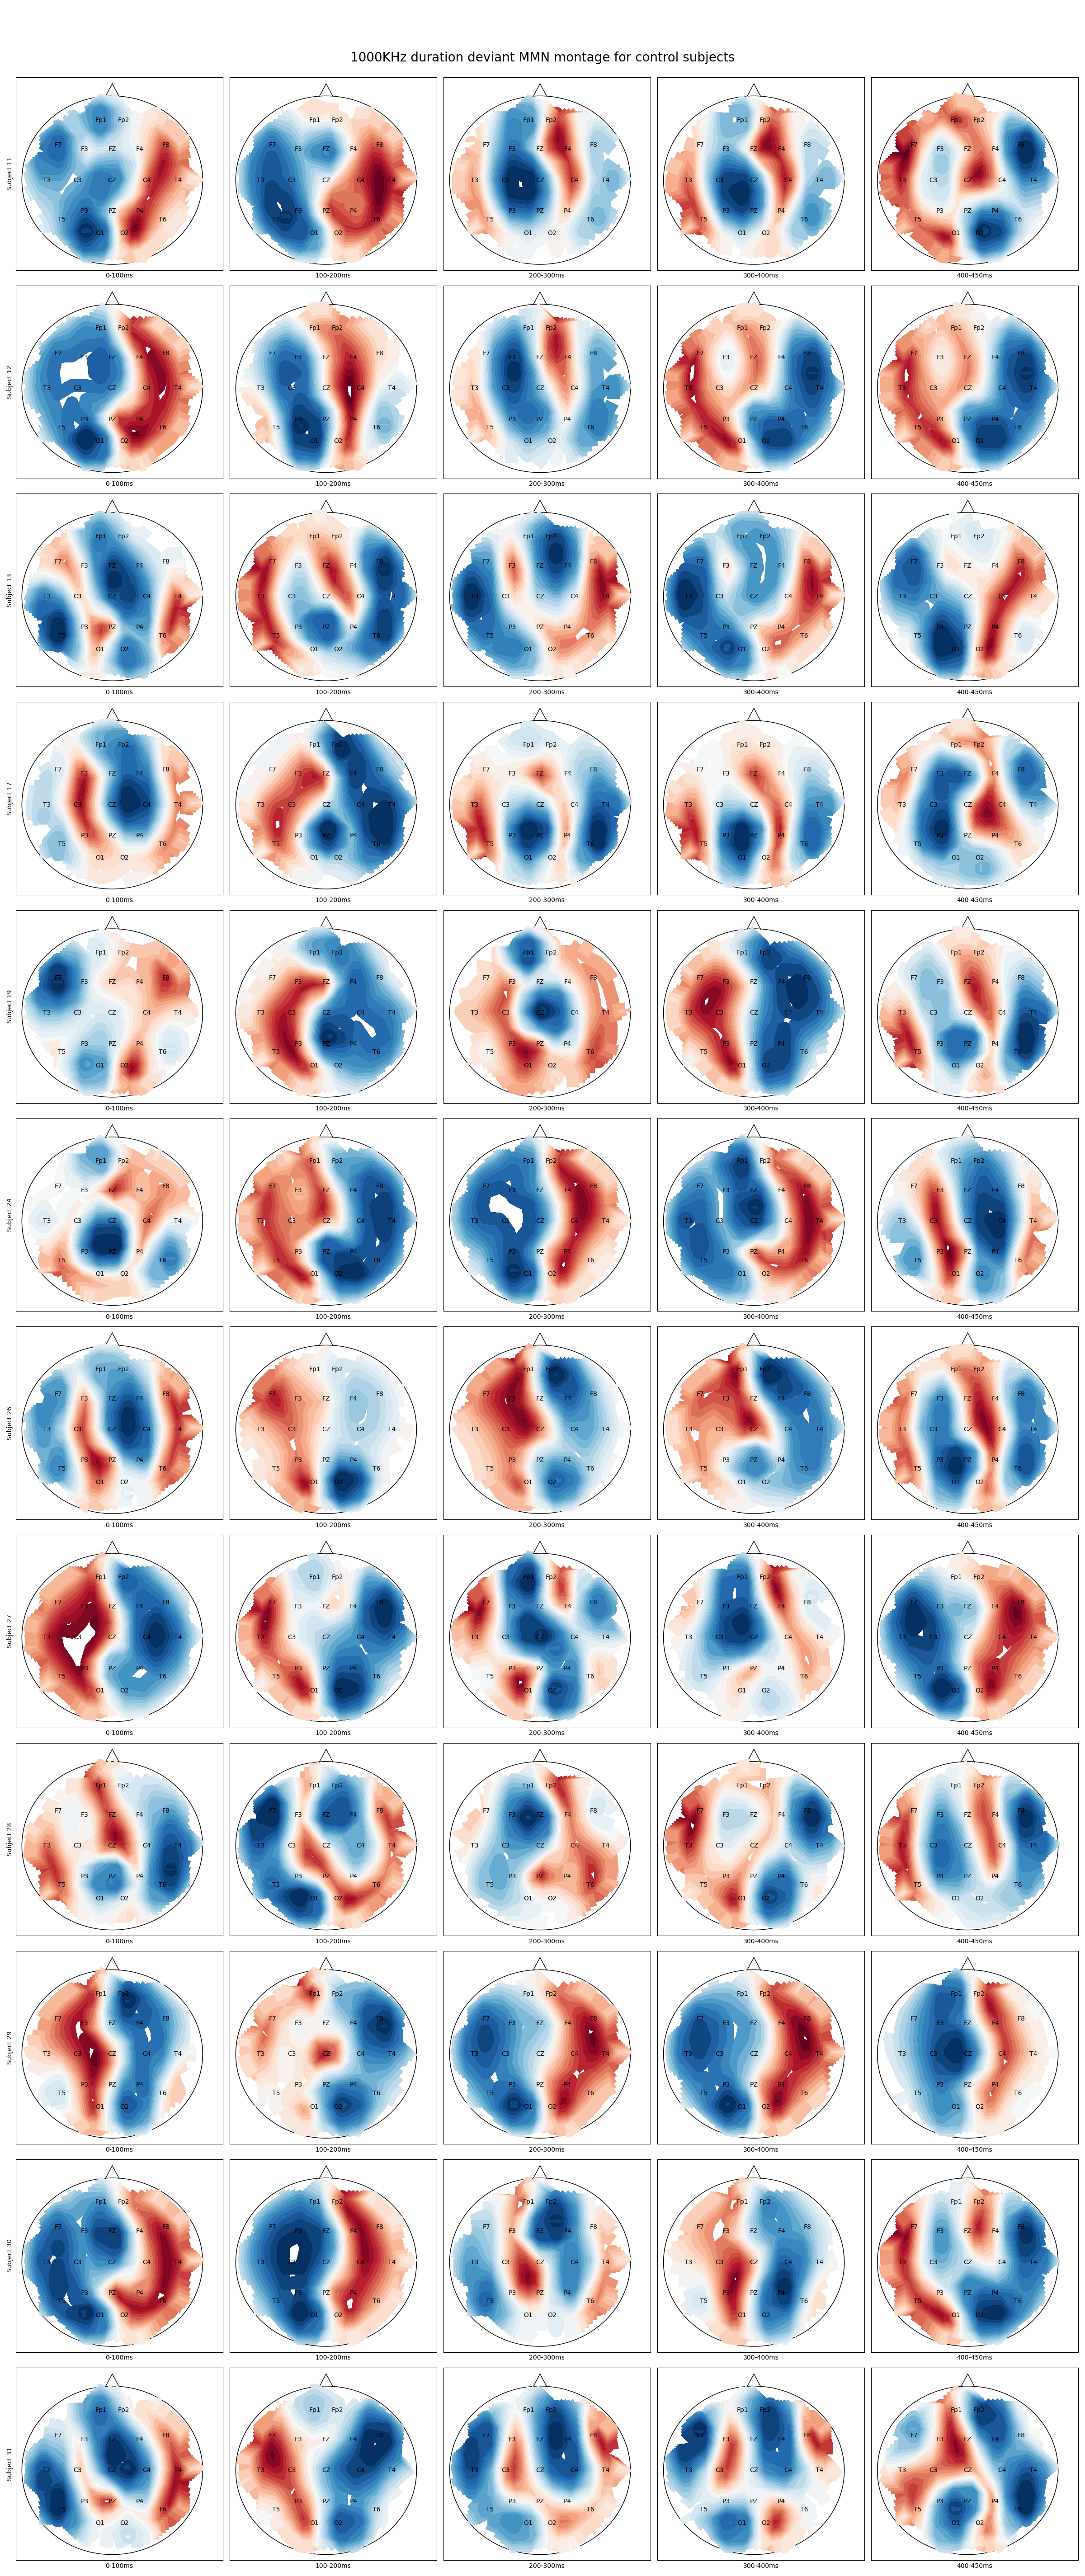
\includegraphics[width=16cm]{../../../data_analysis_results/MMN/montage/Control/1KHz_duration_deviant_montage.png}
  \caption{Controls 1KHz duration deviant \gls{mmn} value montage}\label{control_1KHz_mmn_montage}
\end{figure}
\begin{figure}[H]
  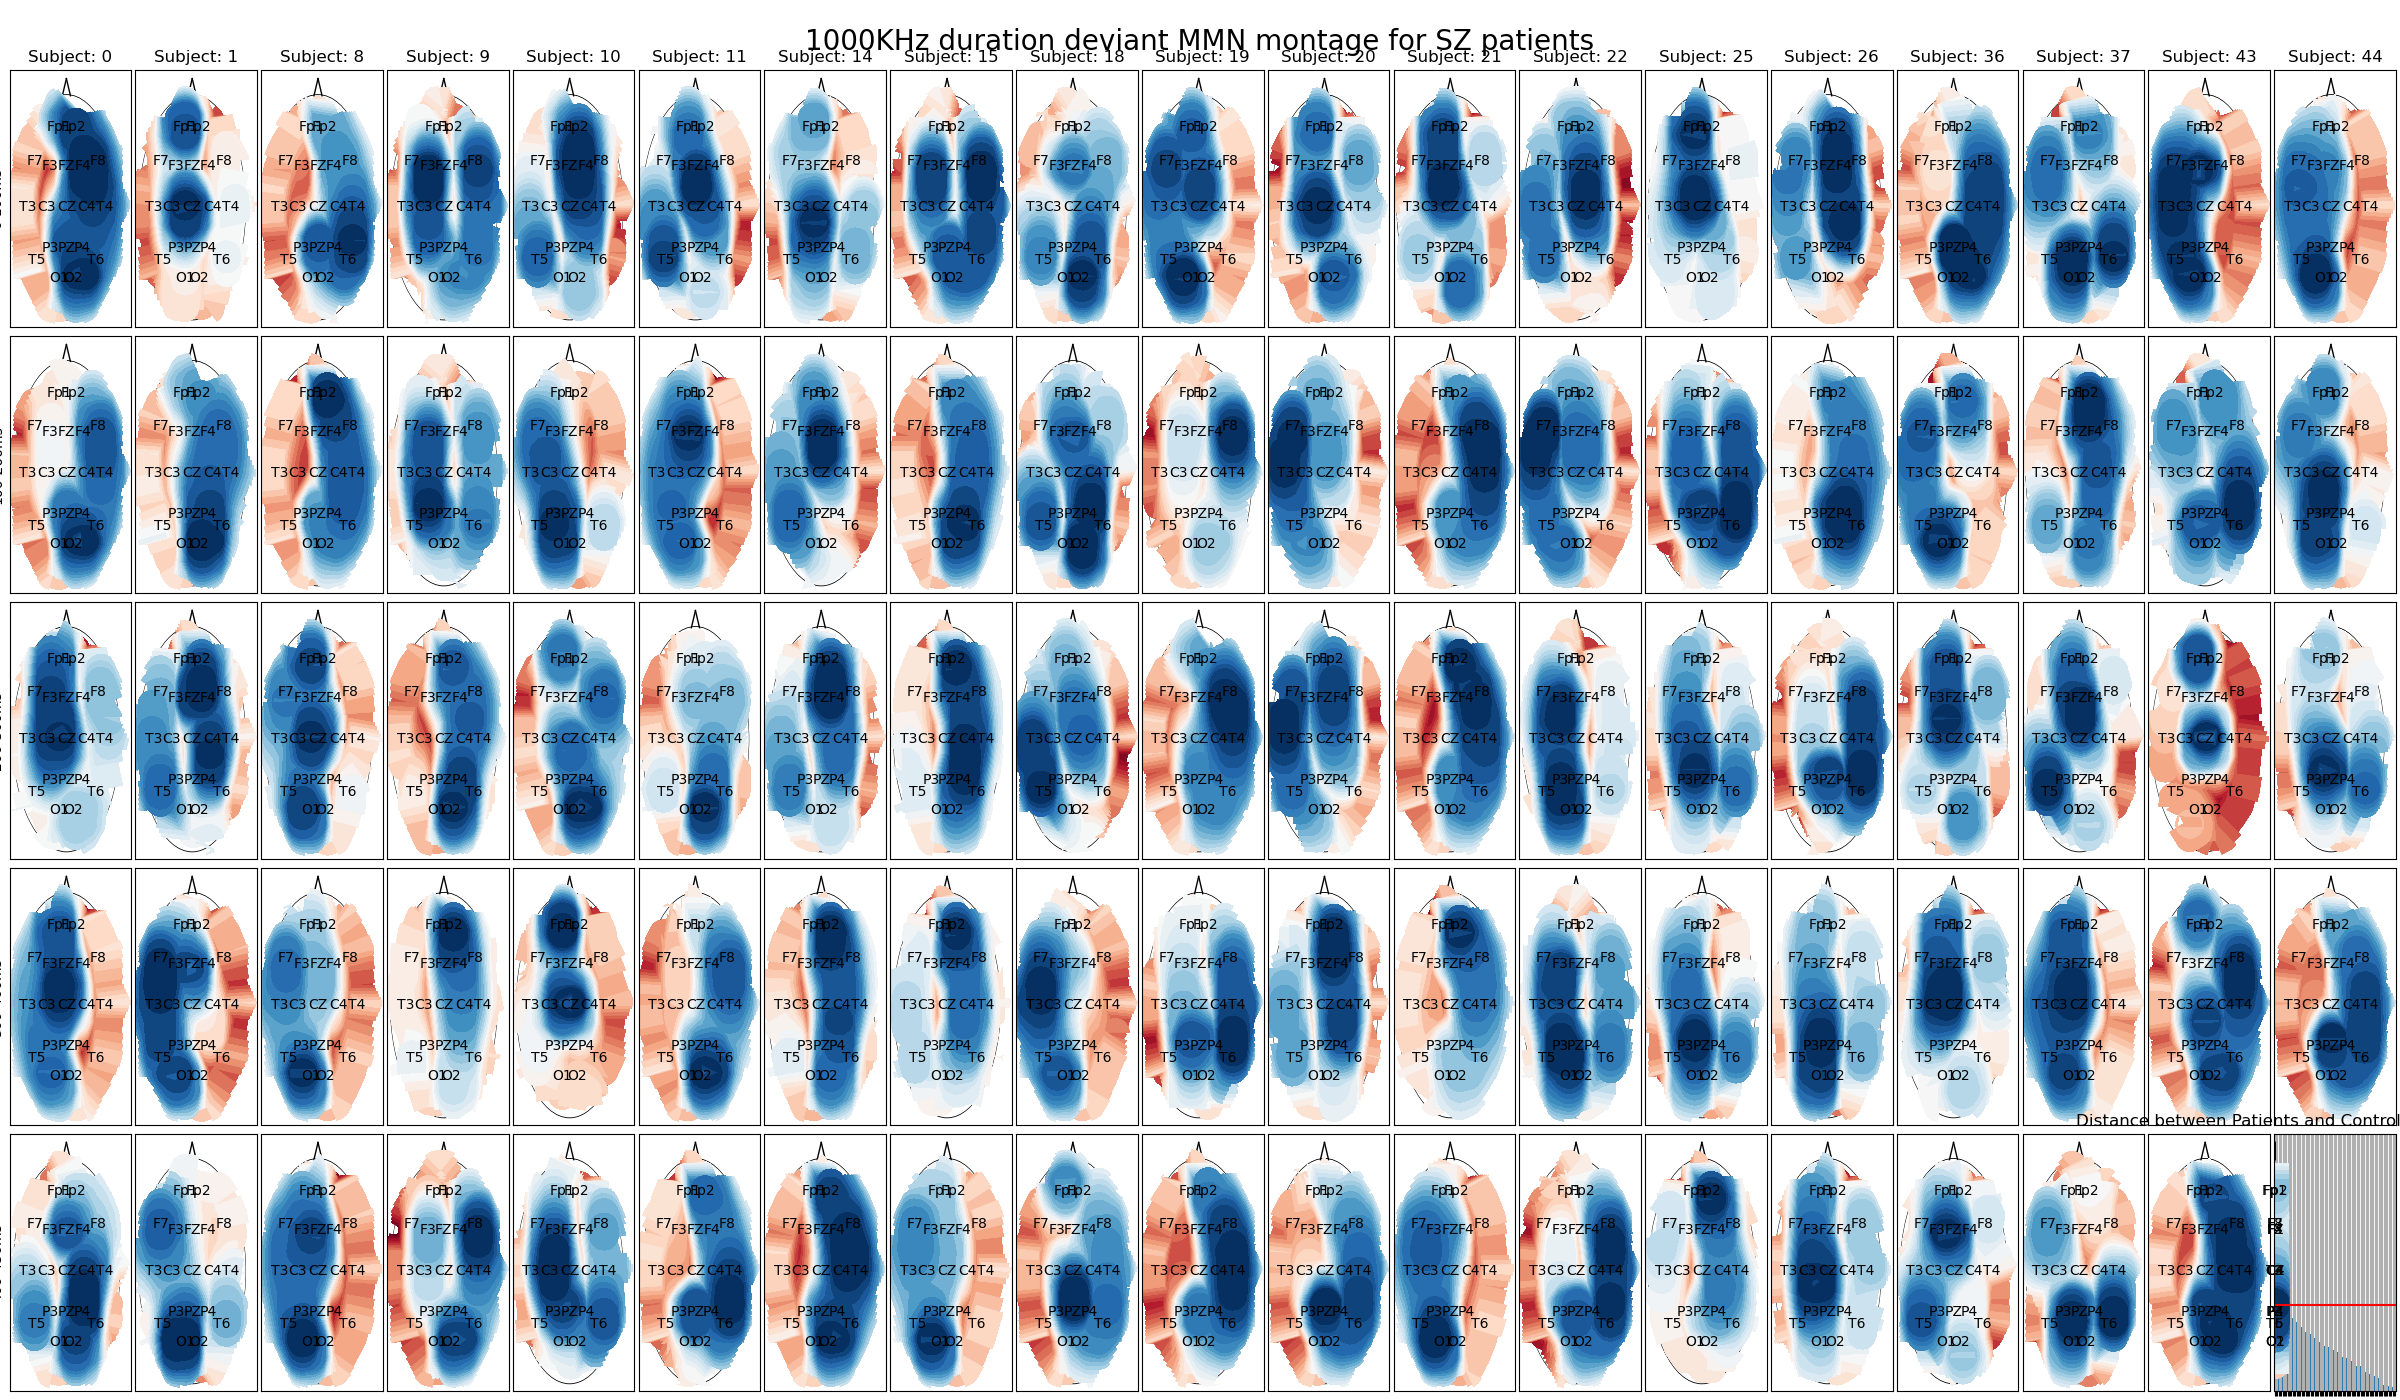
\includegraphics[width=16cm]{../../../data_analysis_results/MMN/montage/Patient/1KHz_duration_deviant_montage.png}
  \caption{Patients 1KHz duration deviant \gls{mmn} value montage}\label{patient_1KHz_mmn_montage}
\end{figure}
\begin{figure}[H]
  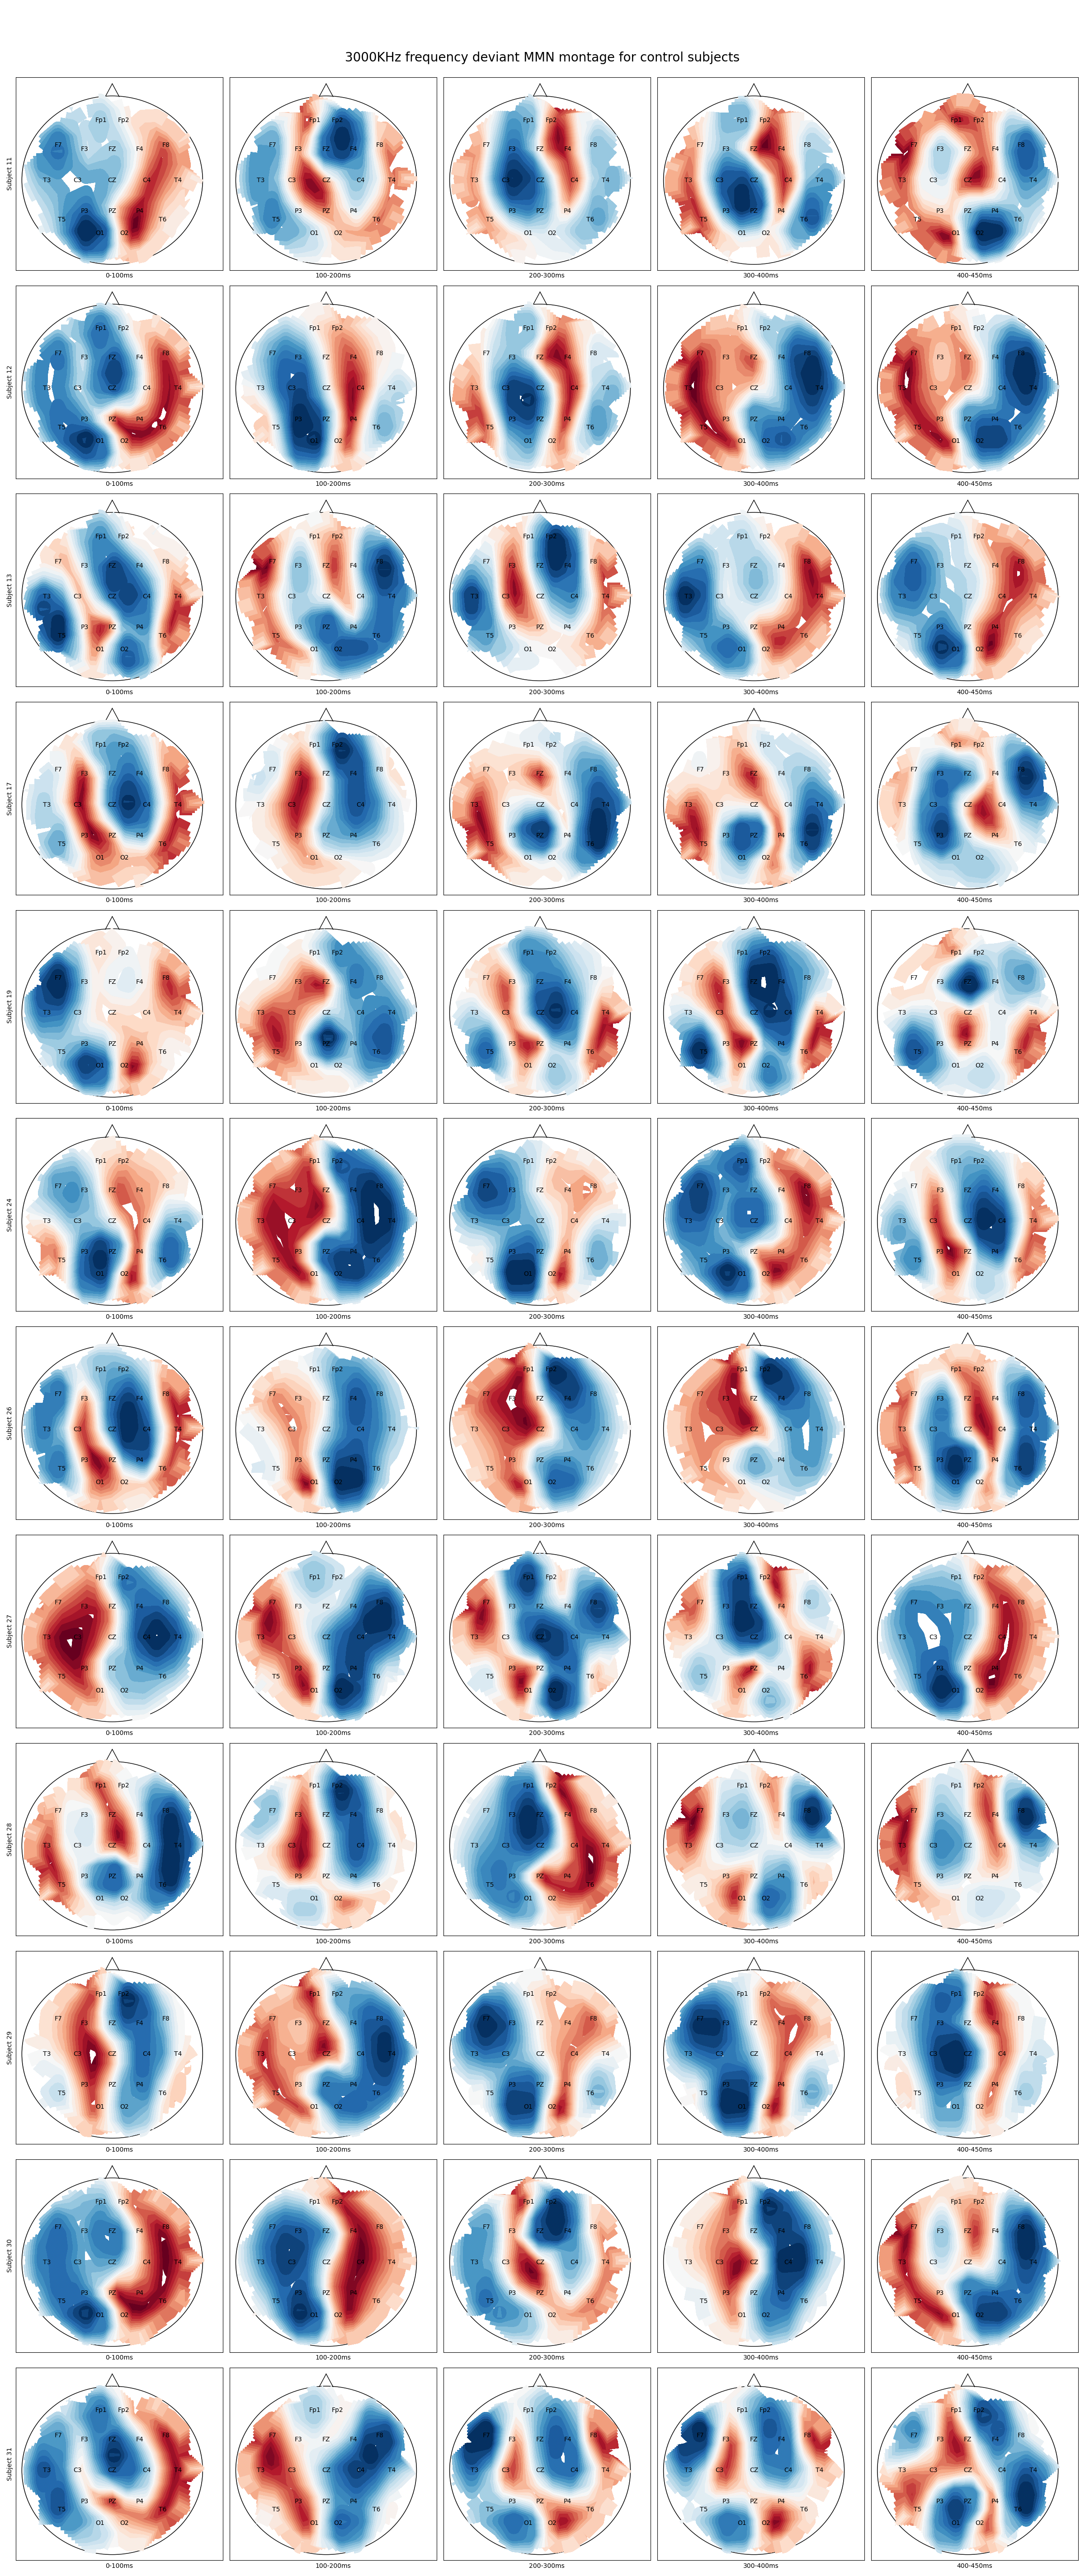
\includegraphics[width=16cm]{../../../data_analysis_results/MMN/montage/Control/3KHz_frequency_deviant_montage.png}
  \caption{Controls 3KHz frequency deviant \gls{mmn} value montage}\label{control_3KHz_mmn_montage}
\end{figure}
\begin{figure}[H]
  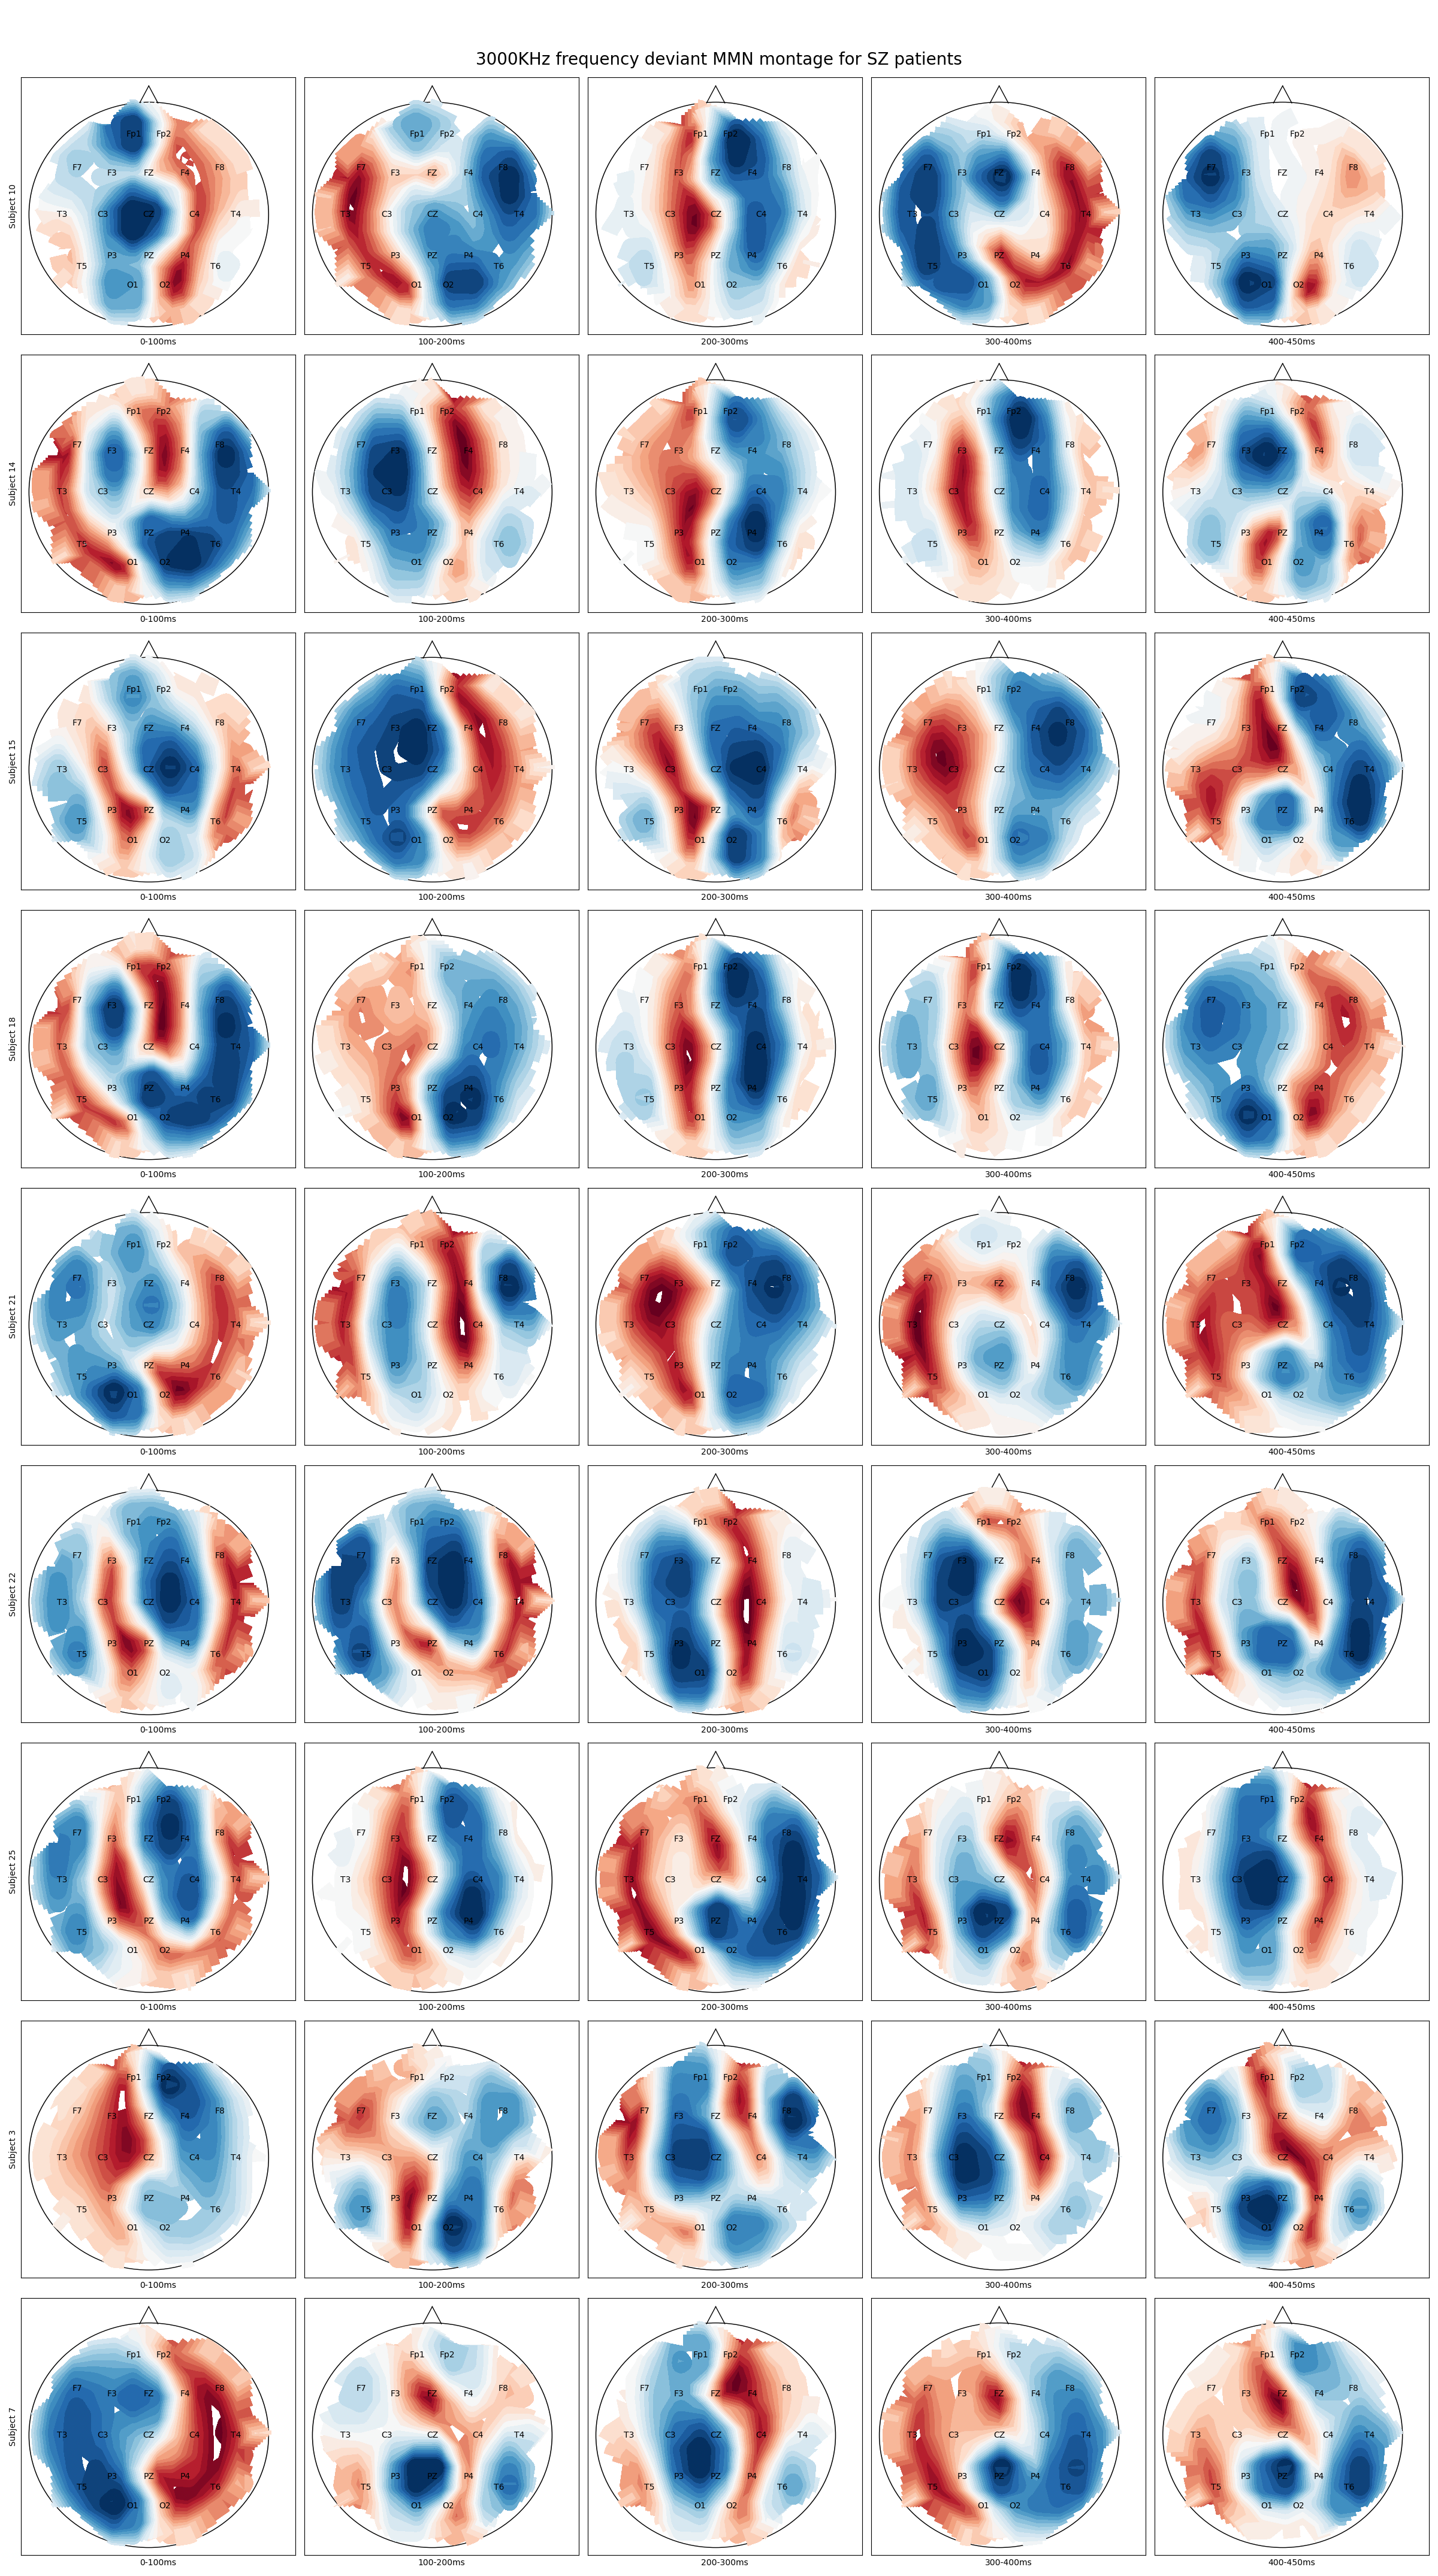
\includegraphics[width=16cm]{../../../data_analysis_results/MMN/montage/Patient/3KHz_frequency_deviant_montage.png}
  \caption{Patients 3KHz frequency deviant \gls{mmn} value montage}\label{patient_3KHz_mmn_montage}
\end{figure}

\begin{figure}[H]
  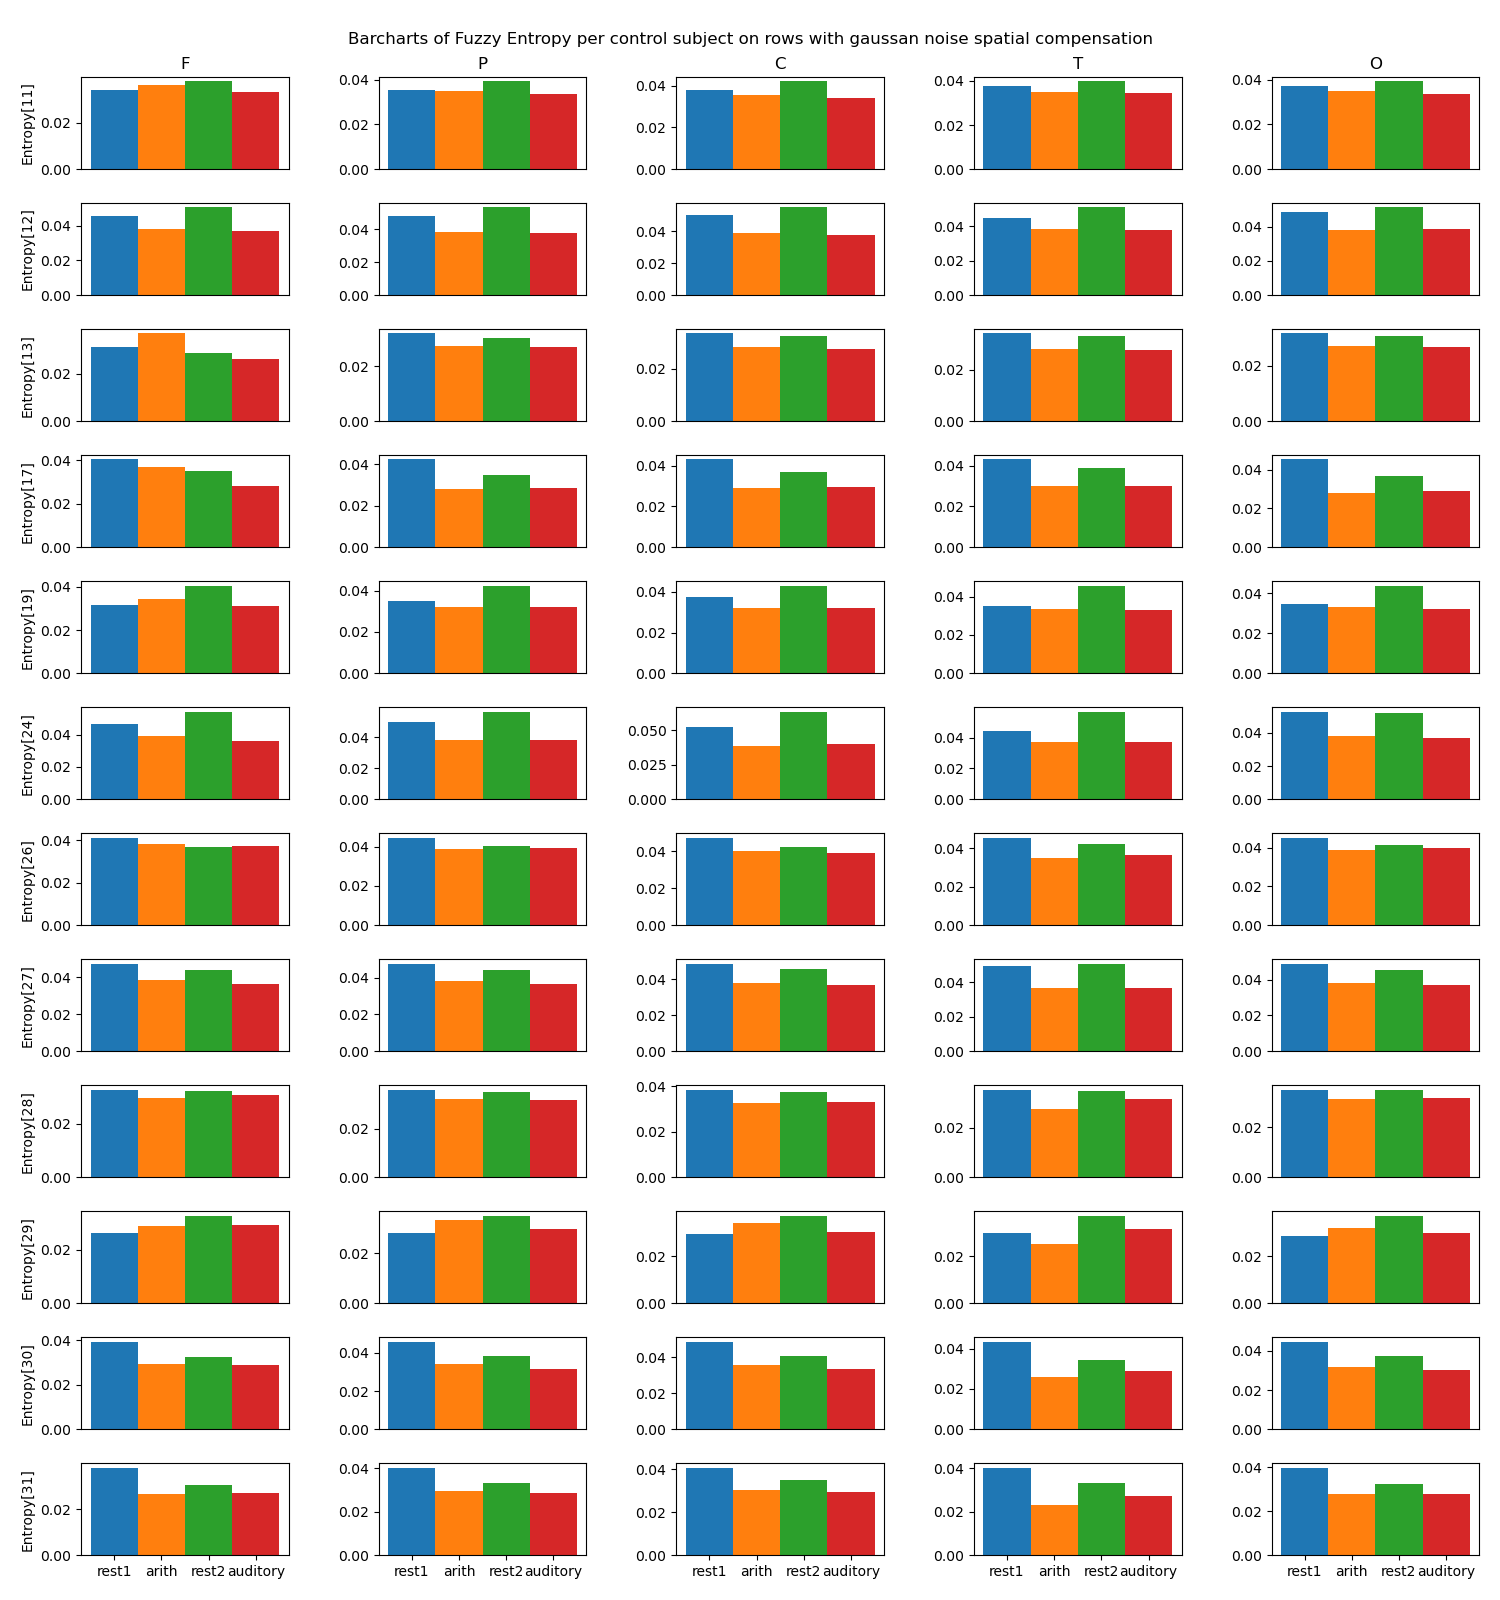
\includegraphics[width=16cm]{../../../data_analysis_results/FuzzEnt/Control/all-fuzzyEntr.png}
  \caption{Fuzzy Entropy from controls}\label{fig:controlFuzzEnt}
\end{figure}
\begin{figure}[H]
  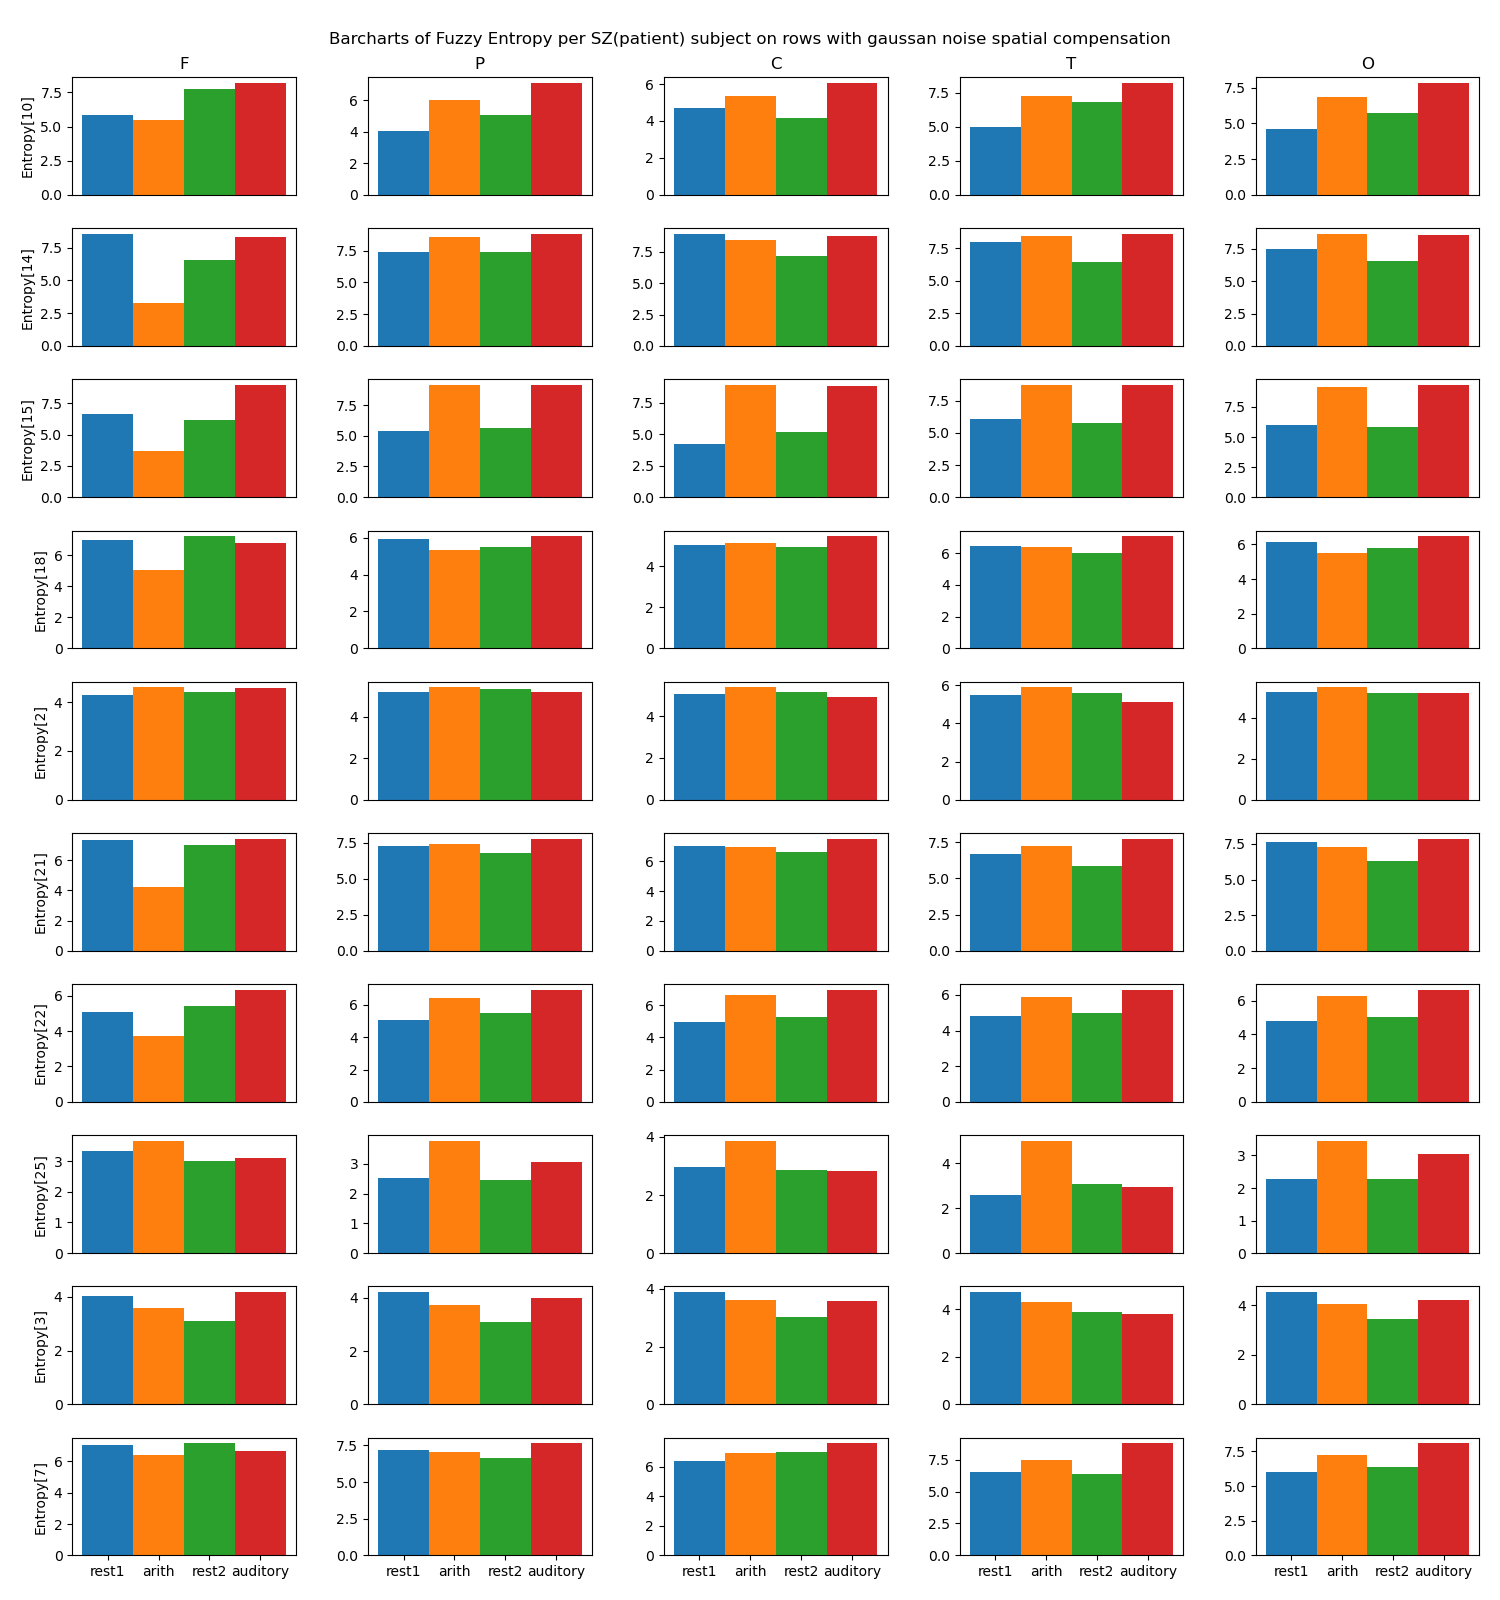
\includegraphics[width=16cm]{../../../data_analysis_results/FuzzEnt/Patient/all-fuzzyEntr.png}
  \caption{Fuzzy Entropy from patients}\label{fig:patientFuzzEnt}
\end{figure}
\begin{figure}[H]
  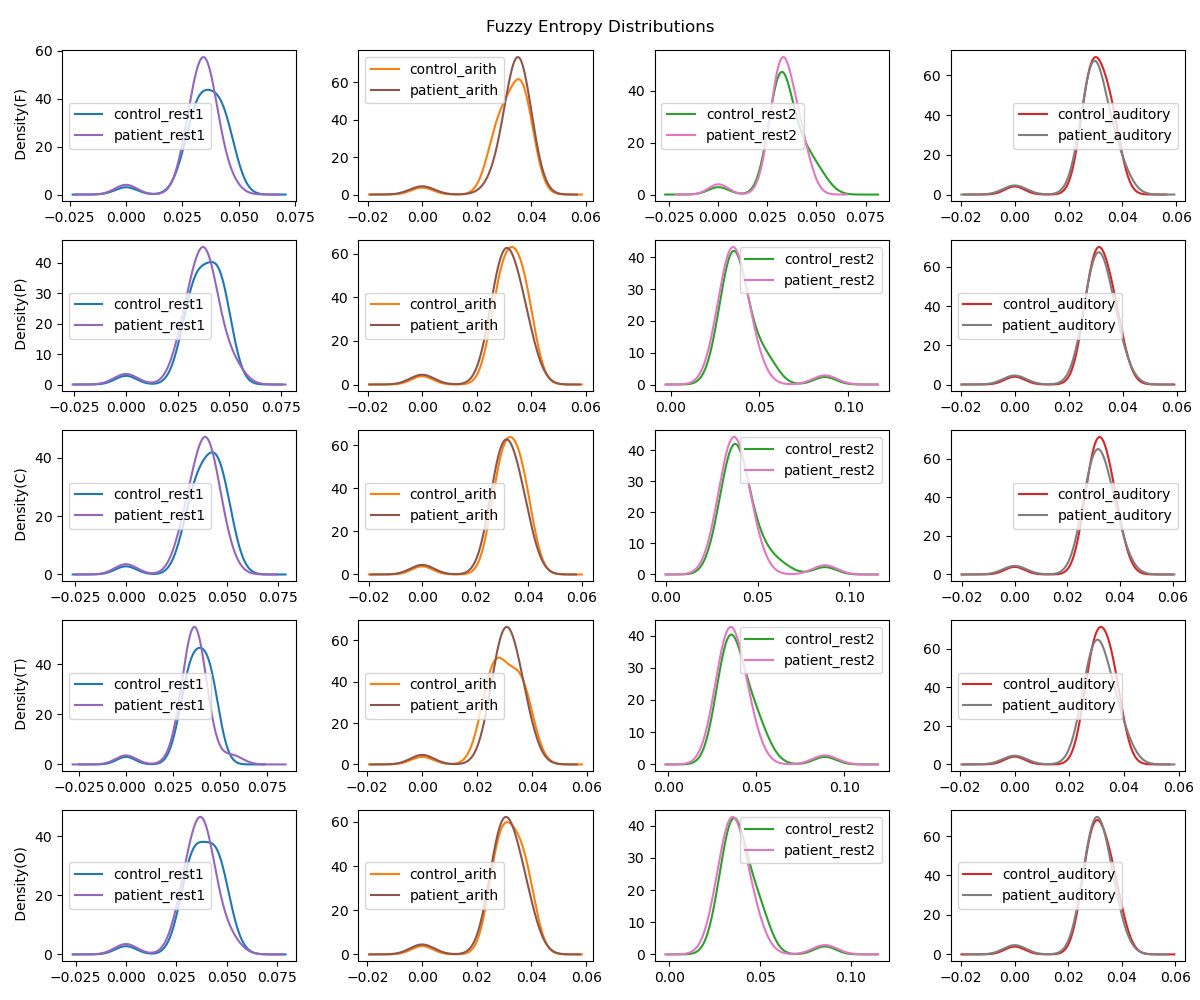
\includegraphics[width=16cm]{../../../data_analysis_results/FuzzEnt/corticalRegions_DAQphase_distributions.png}
  \caption{Fuzzy Entropy from controls}\label{fuzz_ent_distributions}
\end{figure}

\begin{figure}[H]
  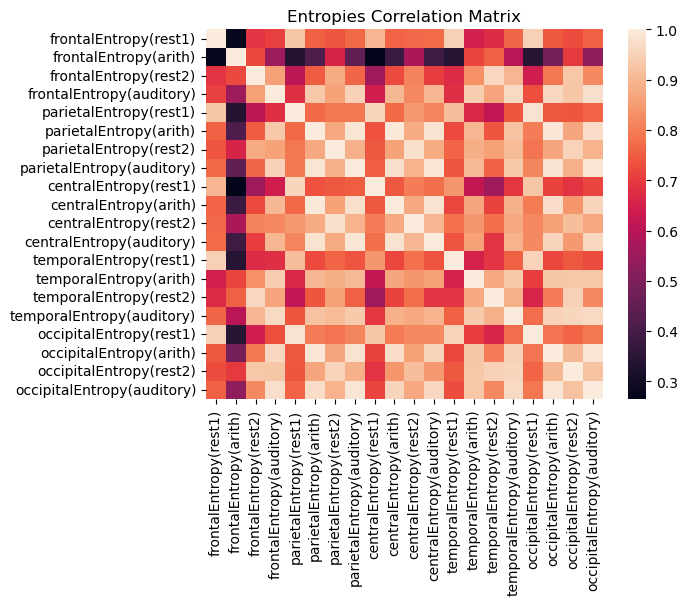
\includegraphics[width=16cm]{../../../data_analysis_results/FuzzEnt/entropies_corr_mat.png}
  \caption{Fuzzy-entropy values correlation smatrix}\label{fuzz_ent_corr_mat}
\end{figure}

\begin{figure}[H]
  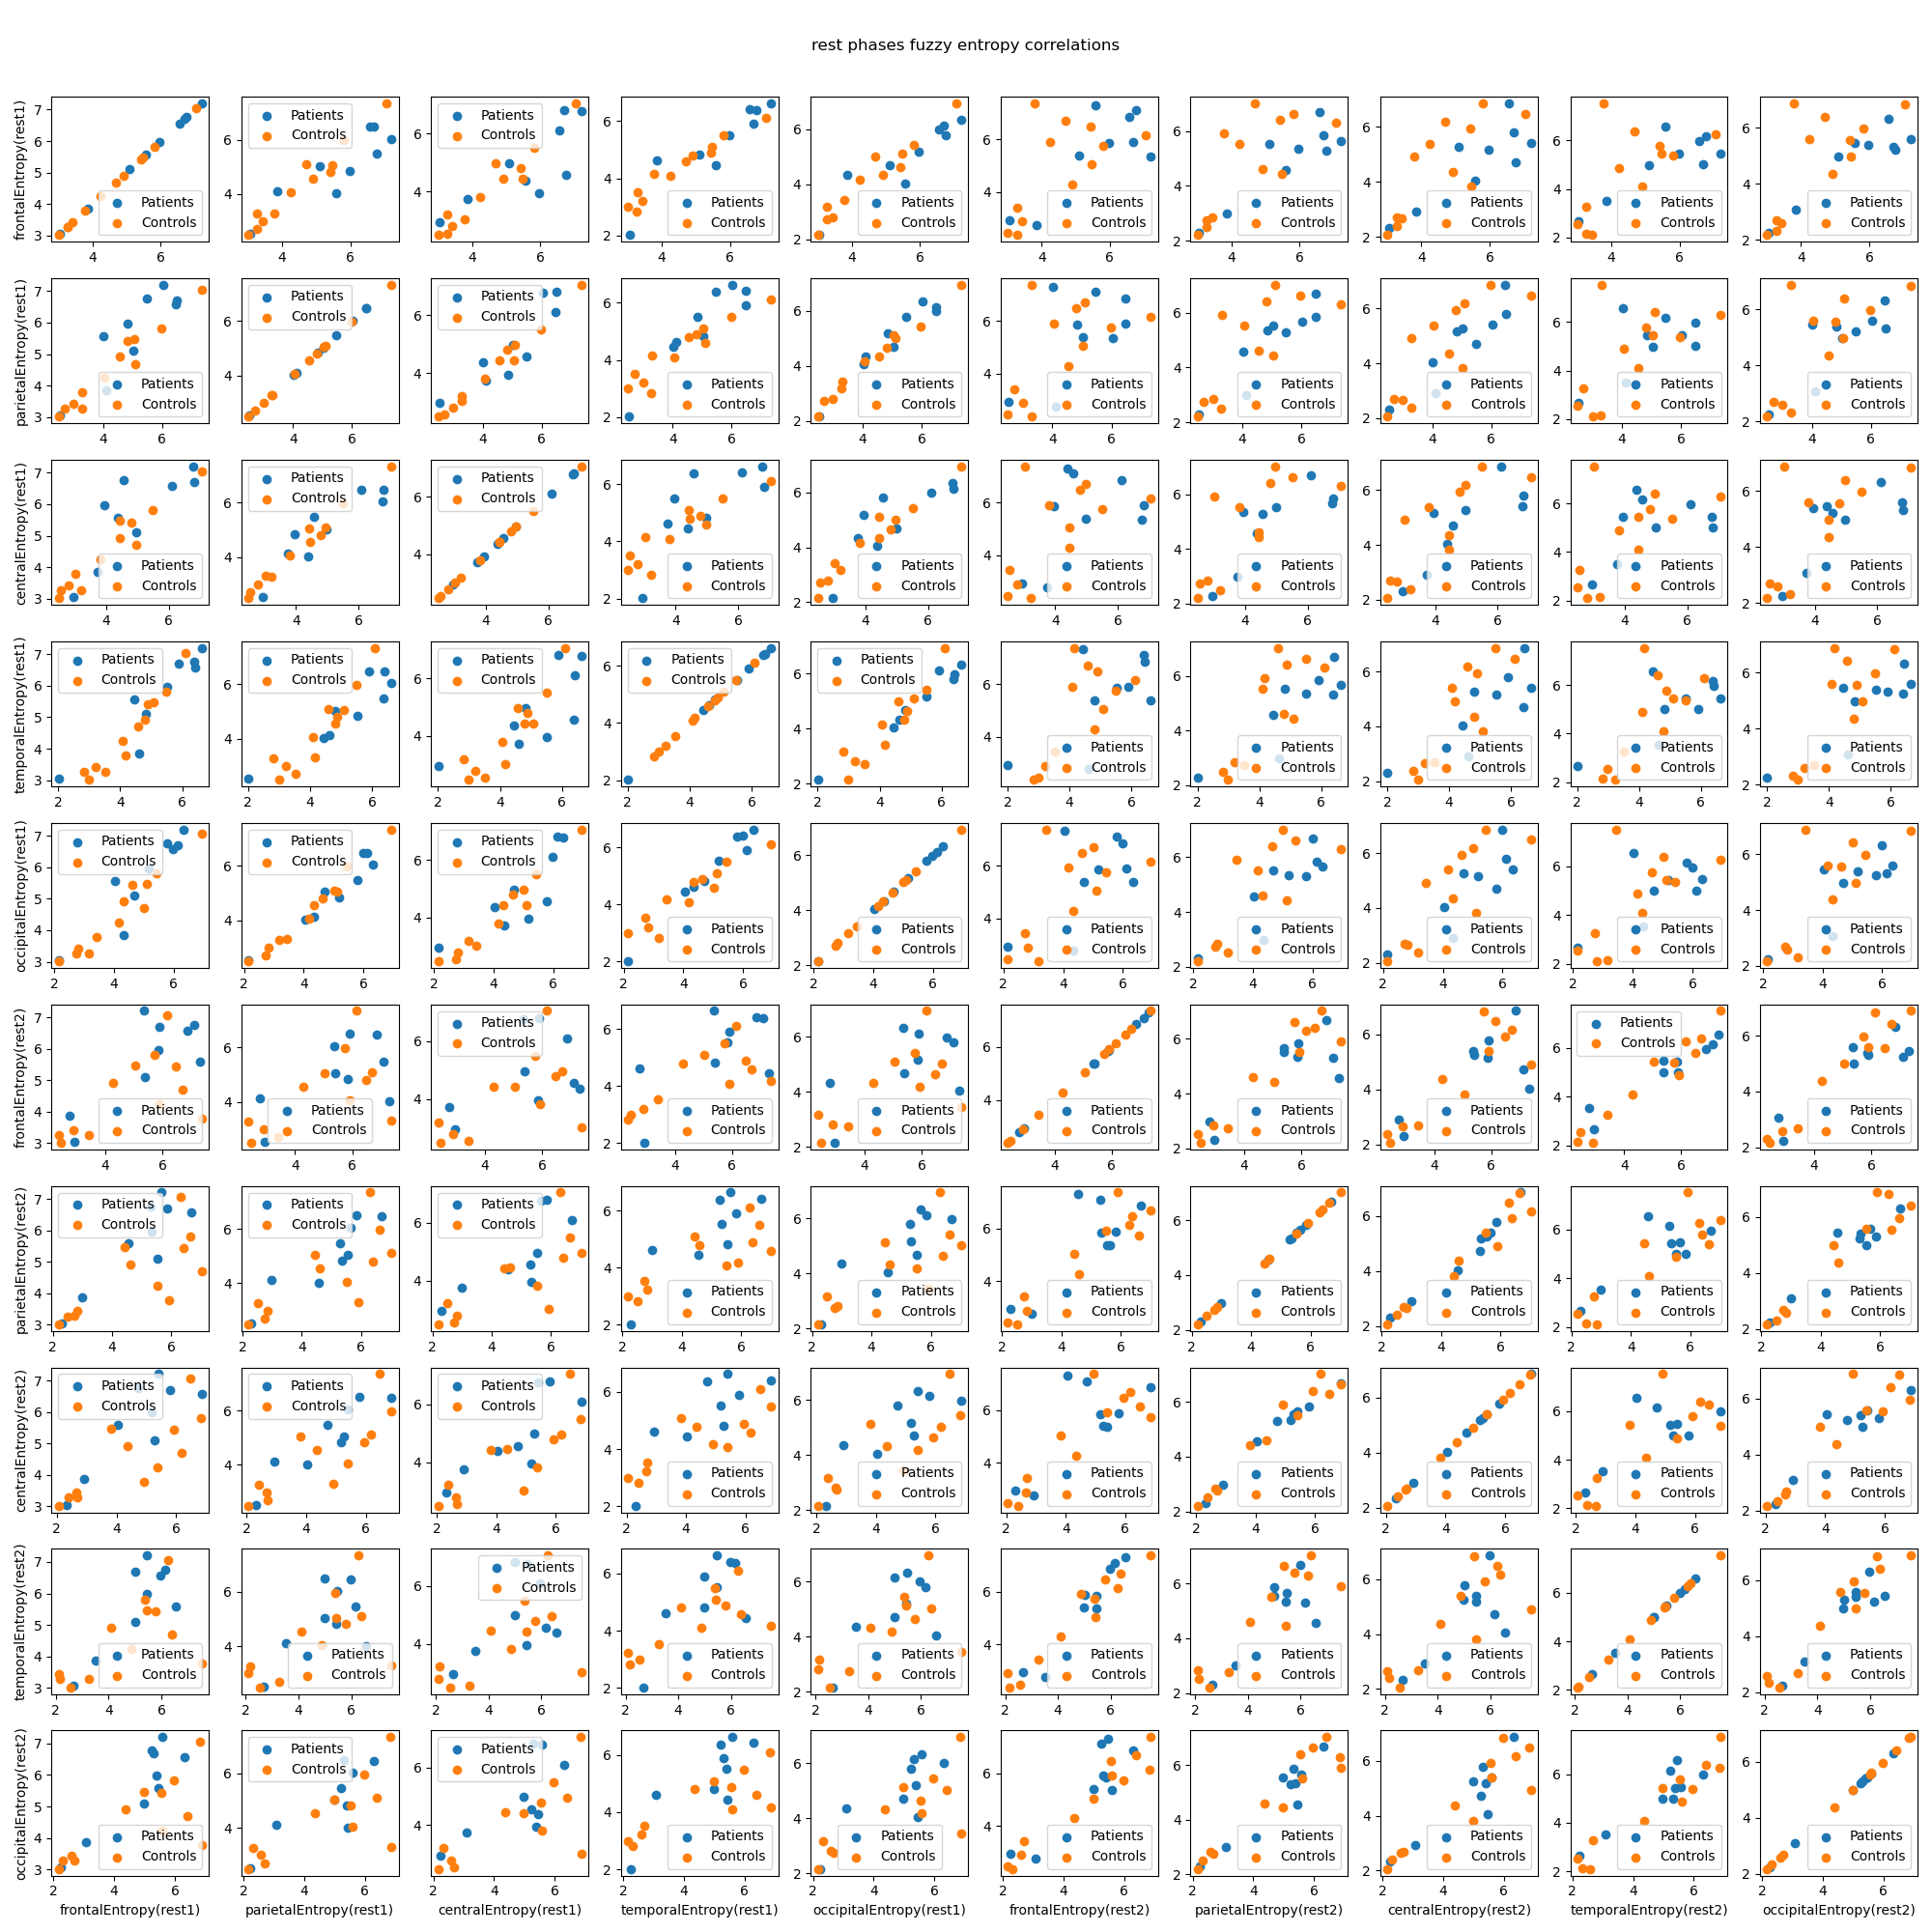
\includegraphics[width=16cm]{../../../data_analysis_results/FuzzEnt/rest_phases_corr.png}
  \caption{Rest Phases Fuzzy-entropy}\label{rest_fuzz}
\end{figure}
\begin{figure}[H]
  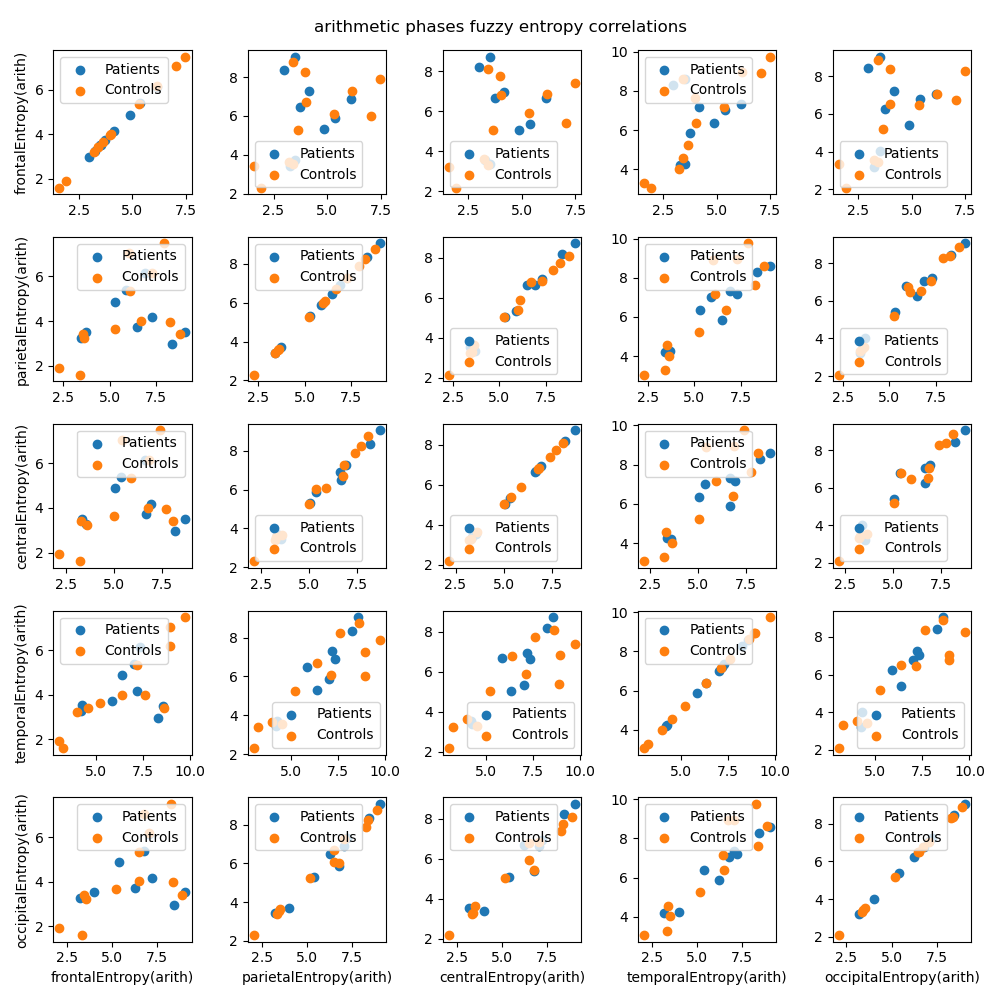
\includegraphics[width=16cm]{../../../data_analysis_results/FuzzEnt/arith_phases_corr.png}
  \caption{Arithmetic Phase Fuzzy-entropy}\label{arith_fuzz}
\end{figure}
\begin{figure}[H]
  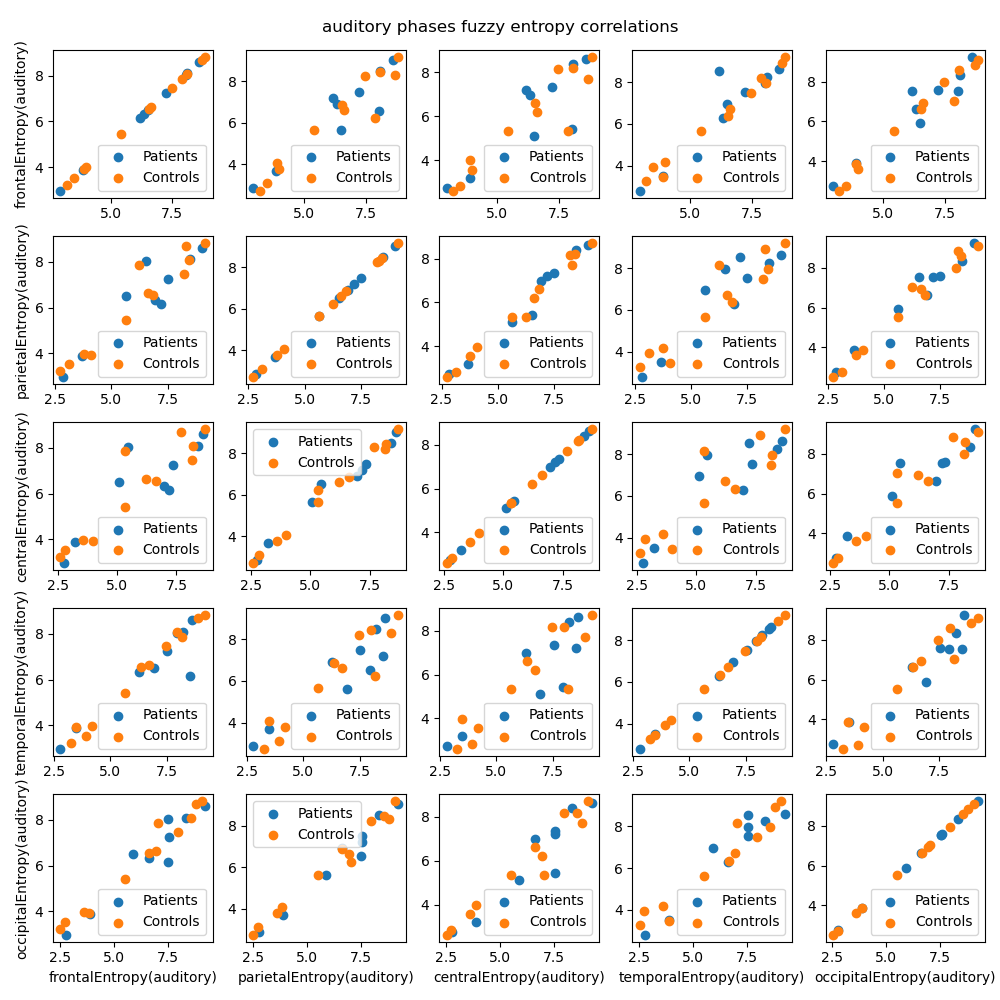
\includegraphics[width=16cm]{../../../data_analysis_results/FuzzEnt/auditory_phases_corr.png}
  \caption{Auditory Phase Fuzzy-entropy}\label{auditory_fuzz}
\end{figure}

\begin{figure}[H]
  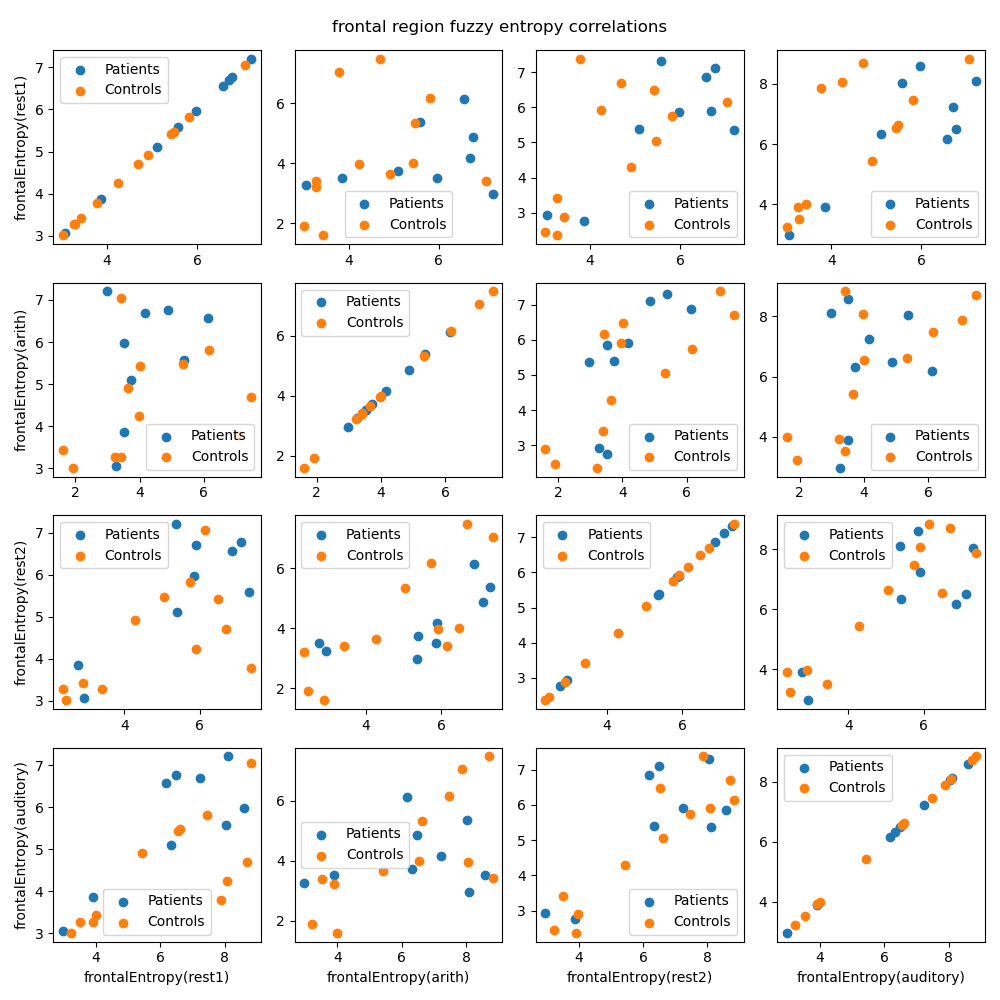
\includegraphics[width=16cm]{../../../data_analysis_results/FuzzEnt/frontal_region_corr.png}
  \caption{Frontal lobe Fuzzy-entropy}\label{frontal_fuzz}
\end{figure}
\begin{figure}[H]
  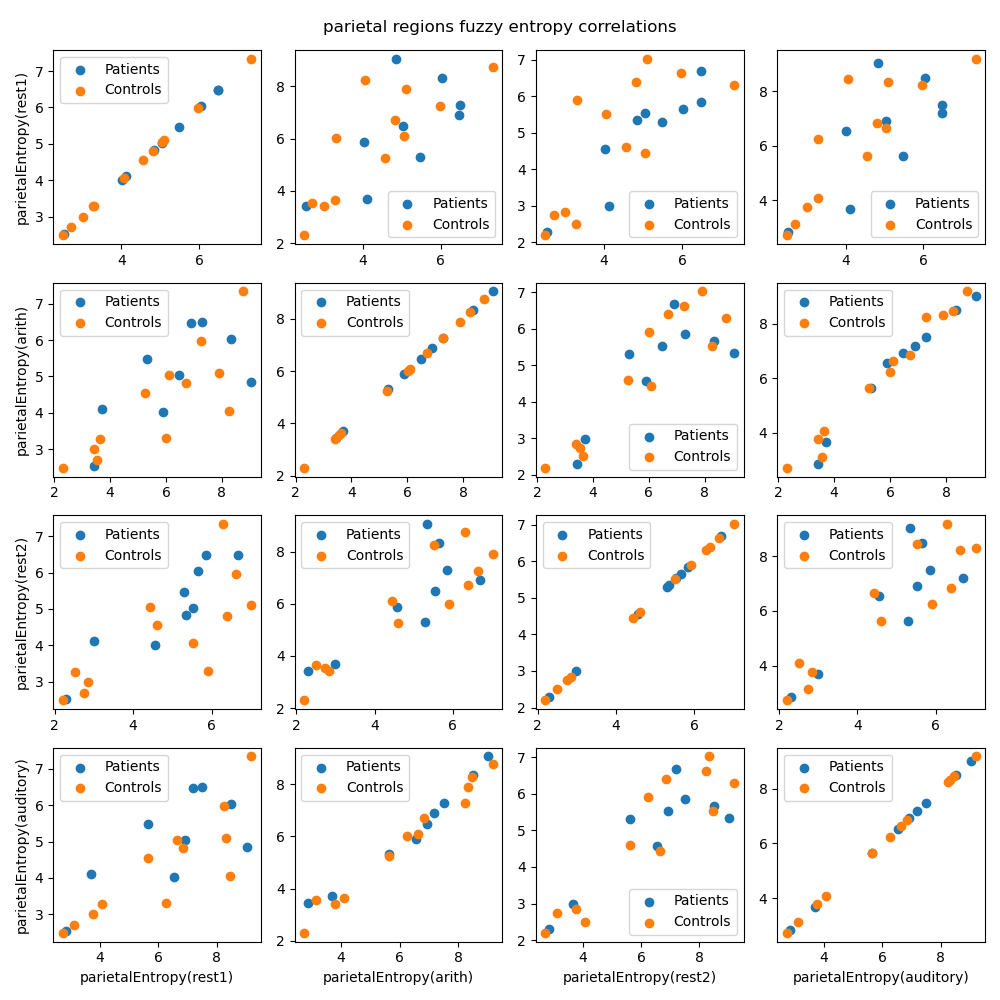
\includegraphics[width=16cm]{../../../data_analysis_results/FuzzEnt/parietal_region_corr.png}
  \caption{Parietal lobe Fuzzy-entropy}\label{parietal_fuzz}
\end{figure}
\begin{figure}[H]
  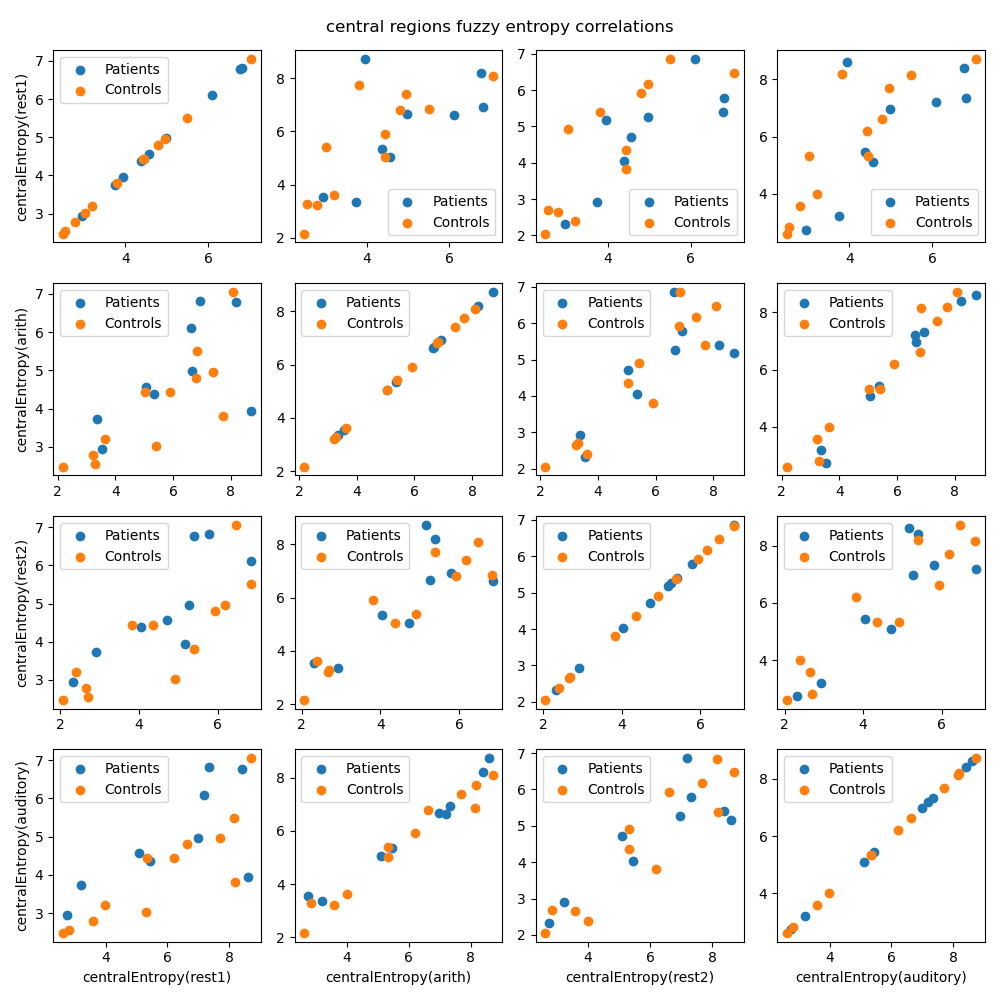
\includegraphics[width=16cm]{../../../data_analysis_results/FuzzEnt/central_region_corr.png}
  \caption{Central lobe Fuzzy-entropy}\label{central_fuzz}
\end{figure}
\begin{figure}[H]
  \includegraphics[width=16cm]{../../../data_analysis_results/FuzzEnt/occipital_region_corr.png}
  \caption{Occipital lobe Fuzzy-entropy}\label{occipital_fuzz}
\end{figure}
\begin{figure}[H]
  \includegraphics[width=16cm]{../../../data_analysis_results/FuzzEnt/temporal_region_corr.png}
  \caption{Temporal lobe Fuzzy-entropy}\label{temporal_fuzz}
\end{figure}

\end{document}
% \include{monthlly_report.acn}

%\journal{CSc 4110 Final Report}

%\title[journalExample]{Format for Project Reports}
\title{
  An update on the project: 
  \textbf{
      \textit{
        Development of an Automatic Instrument for Schizophrenia(SZ) Diagnosis
        }
      }, for the MCIP Innovation Prize 2022.
  }
% \author{
% Emmanuel OLATEJU \\
%     \begin{affiliation}
%       Supervised by Dr. K.P. Ayodele \\ 14/02/2023, \\
%       email: \mbox{kayodele@gmail.com, eoolateju@student.oauife.edu.ng}
%     \end{affiliation}
% }

\begin{document}
\maketitle

\section{Overview}
The purpose of this project is to design an instrument for early \gls{sz} diagnosis.
In designing the instrument, the following parts are to be developed:
\begin{itemize}
  \item An \gls{eeg} \gls{daq} system
  \item \gls{daq} user interface.
  \item Hand-clicker device for \gls{daq} process feedback from patient and clinicians.
  \item Machine/deep learning model.
  \item Soft instrument interacting with learnt model, \gls{daq} software, handheld 
  clicker, \gls{eeg} headbox and all developed parts.
  
\end{itemize}
The goal is to develop a medical turnkey device for \gls{sz} diagnosis having its own 
\gls{eeg} device and deeply embedded software. The long-term goal is for this turnkey device 
and its software to be built around the OpenBCI \gls{eeg} kit. The OpenBCI is chosen as
minimal number of electrode sites needed for \gls{sz} diagnosis may be identified and thus 
an \gls{eeg} kit that allows for flexibility of electrodes to be used is needed. This will 
mitigate the cost of the device making it more accessible. In the short term, the contec 
\gls{eeg} headbox is being used in identifying the best electrode sites.

The contec \gls{eeg} headbox is being used in place of the OpenBCI headbox temporarily 
for generation of the \gls{eeg} signals.
In order to fetch \gls{eeg} signals from the headbox, a piece of software that interacts 
with the contec's firmware has been developed. This piece of software has been incorporated 
with a user interface developed that makes \gls{daq} sessions interactive for both 
subjects and clinicians. The user interface and firmware interacting code together make 
up the Generis software presented in the first report.

In order to make \gls{daq} sessions more interactive, a handheld clicker is being developed 
to help patients and clinicians give feedback to the Generis software. Annotations can be 
somewhat a tough technical task and in certain cases becomes an headache for non-technical 
users. Once annotation messagess are configured into this clicker device, adding annotations 
will be redced to a task of simply clicking color coded buttons. This piece of hardware 
will also improve processing of signals as time during \gls{daq} of noise causing actions can be 
annotated and also times of subject inactivity or inert state to \gls{daq}. The handheld clicker 
is able to communicate with the Generis software through UART to USB communication.

In order to have an instrument of high accuracy and to solve the problem of \gls{sz} diagnosis 
being based on psychiatric nosology, the instrument(model) must be calibrated to seperate 
\glspl{szPtnt} from \glspl{hc}. This is being done using machine-learning and/or 
deep-learning methods and signal-processing algorithms to extract information relevant to 
\gls{sz} measurement and to improve discriminability.

The final instrument that integrates all of the designed parts is to be devloped upon 
completion of the handheld clicker and complete development of model to be used in 
measuring the extent of \gls{sz} disorder and classification of subjects. The structure 
of the final instrument is shown in the diagram below.
\begin{figure}[H]
  \includegraphics[width=16cm]{../../../images/technical/instrument.drawio.png}
  \caption{\gls{sz} diagnosis instrument}\label{instrument}
\end{figure}


\section{Handheld clicker}
The handheld clicker design is based on an arduino nano which applies the output of four 
tact switches as inputs to four vectored interrupts on the nano development board. The 
exact labels of these inputs has not been assigned as a study of the erogonomics of 
conventions employed in other devices of this kind and how best conventions are adapted and 
modified for the use case of this project is being studied. 

The current design of the handheld clicker(annotator) is the second iteration and is referred 
to as HC-v0.2. 
The circuit diagram of the handheld clicker is given in figure \ref{clicker_circuit}.
The flowchart describing the algorithm of this device is shown in figure \ref{clicker_flowchart}. 
The front and top images of the hand-clicker-v0.2 are shown in figures \ref{clicker} and 
\ref{top_view_of_clicker}.
\begin{figure}[H]
  \includegraphics[width=16cm]{../../../hardware/handheld_clicker/circuit_image.png}
  \caption{handheld clicker circuit}\label{clicker_circuit}
\end{figure}
\begin{figure}[H]
  \includegraphics[height=16cm,width=10cm]{../../../hardware/handheld_clicker/flowchart.png}
  \caption{Flowchart algorithm of clicker}\label{clicker_flowchart}
\end{figure}
\begin{figure}[H]
  \includegraphics[width=16cm]{../../../hardware/handheld_clicker/front.jpeg}
  \caption{Front view of clicker}\label{clicker}
\end{figure}
\begin{figure}[H]
  \includegraphics[,height=10cm,width=8cm]{../../../hardware/handheld_clicker/top.jpeg}
  \caption{Top view of clicker}\label{top_view_of_clicker}
\end{figure}


\section{Model Development (Feature-extraction, Data-analysis)}
\subsection{Feature Extraction}
March's report presented the fuzzy entropy features extracted from cortical
regions during phases of \gls{daq} and also the refined \gls{mmn} plots which 
made the \gls{mmn} waveform more evident. Relevant changes made to features 
extraction highlighted in marchs's report includes:
\begin{itemize}
  \item Recomputing the \gls{mmn} waveforms
  \item Spatial dimension augmentation with gaussian noise during computation of fuzzy-entropy
  \item Development of custom fuzzy-entropy library
\end{itemize}
The following was proposed as the next set of action points:
\begin{itemize}
  \item The continued improvement of fuzzy-entropy library to work with multivariate \\
  time-series(2D data)
  \item comparing performance of the fuzzy-entropy features from sourced library to \\
  that of the personally developed library
  \item Computing the auditory steady state features
\end{itemize}
A slight detour was made from these proposed action points for the month of april. 
Analysis of the extracted features for levels of dicriminability was carried out 
to understand how to improve the features extraction methods. The analysis shows 
a significant level of discrimination in the \gls{mmn} features, less in the 
fuzzy-entropy features, though the correlation patterns of the fuzzy-entropy features 
suggest they might carry information on extent of \gls{sz} disorder.

\gls{mmn} features have been extracted from the scaled \gls{mmn} waveforms. The 
\gls{mmn} features were computed as the mean of the \gls{mmn} waveforms within 
the time-frames 0-100ms, 100-200ms, 200-300ms, 300-400ms, 400-450ms.

Formerly implemented montage plot algorithm was improved upon to reduce 
time-complexity so as to make data visualization and analysis easier to obtain 
intuitive information from.

\subsection{Data Analysis/Visualization}\label{data_analyis}
 Analysis of the extracted features was done to establish the quality of discriminative 
 and quantitative information contained in the extracted features. The method of 
 Visualization of some of these features changed to make analysis easy.
 The results of the analysis are given in section \ref{figures}. Visualization methods 
 and analysis carried out includes:
\begin{itemize}
  \item Comparing \gls{mmn} feature values for 1KHz duration deviant and 3KHz frequency deviant 
  between patient and controls across all electrodes and time windows.
  (Figures \ref{mmnvalue_0_100ms} - \ref{mmnvalue_400_450ms})
  \item Converting the \gls{mmn} values to montage plots for 1KHz duration deviant 
  and 3KHz frequency deviant for easier interpretation and analyzing montage evolution.
  (Figures \ref{control_1KHz_mmn_montage}-\ref{patient_3KHz_mmn_montage})
  \item Comparing distribution of computed fuzzy-entropy values of patients and controls 
  for each cortical region across all phases of \gls{daq}.
  (Figures \ref{fig:controlFuzzEnt}-\ref{fuzz_ent_distributions}) 
  \item Correlating fuzzy-entropy values from cortical regions across 
  all phases of \gls{daq}.(Figure \ref{fuzz_ent_corr_mat})
  \item Comparing entropies from all cortical regions for each phase of \gls{daq}.
  (Figures \ref{rest_fuzz}-\ref{auditory_fuzz})
  \item Comparing entropies from all phases of \gls{daq} for each cortical region.
  (figures \ref{frontal_fuzz}-\ref{temporal_fuzz})
\end{itemize} 

\section{Inference and Action Points}
\subsection{Inference}
From the analysis carried out, the \gls{mmn} features of both tone deviants show 
discriminative properties between the \gls{szPtnt} and \gls{hc} in localized head 
regions. The fuzzy-entropy features do not show discriminative abilities, but their 
correlation patterns indicate a linear relationship that might be a measure of degree 
of \gls{sz} disorder. Therefore we need to find methods that improve quality of extracted 
features and proceed with developing a learner model.

\subsection{Action Points}
Based on the inference drawn, the action points for the month of may is as follows:
\begin{itemize}
  \item Computing the auditory steady state features.
  \item Re-computing fuzzy-entropy features using other libraries and 
  comparing performance.
  \item Improve discriminability of features using spatial filters and dimensionality 
  reduction techniques.
  \item Compare performance of a custom mutilayer feedforward network and traditional 
  machine-learning algorithms for classification and estimation of measures of degree 
  of \gls{sz} disorder.
\end{itemize}

\section{Figures}\label{figures}

\begin{figure}[H]
  \includegraphics[width=16cm]{../../../data_analysis_results/MMN/features/deviant_tone_0.png}
  \caption{\gls{mmn} values from 0-100ms}\label{mmnvalue_0_100ms}
\end{figure}
\begin{figure}[H]
  \includegraphics[width=16cm]{../../../data_analysis_results/MMN/features/deviant_tone_1.png}
  \caption{\gls{mmn} values from 100-200ms}\label{mmnvalue_100_200ms}
\end{figure}
\begin{figure}[H]
  \includegraphics[width=16cm]{../../../data_analysis_results/MMN/features/deviant_tone_2.png}
  \caption{\gls{mmn} values from 200-300ms}\label{mmnvalue_200_300ms}
\end{figure}
\begin{figure}[H]
  \includegraphics[width=16cm]{../../../data_analysis_results/MMN/features/deviant_tone_3.png}
  \caption{\gls{mmn} values from 300-400ms}\label{mmnvalue_300_400ms}
\end{figure}
\begin{figure}[H]
  \includegraphics[width=16cm]{../../../data_analysis_results/MMN/features/deviant_tone_4.png}
  \caption{\gls{mmn} values from 400-450ms}\label{mmnvalue_400_450ms}
\end{figure}

\begin{figure}[H]
  \includegraphics[width=16cm]{../../../data_analysis_results/MMN/montage/Control/1KHz_duration_deviant_montage.png}
  \caption{Controls 1KHz duration deviant \gls{mmn} value montage}\label{control_1KHz_mmn_montage}
\end{figure}
\begin{figure}[H]
  \includegraphics[width=16cm]{../../../data_analysis_results/MMN/montage/Patient/1KHz_duration_deviant_montage.png}
  \caption{Patients 1KHz duration deviant \gls{mmn} value montage}\label{patient_1KHz_mmn_montage}
\end{figure}
\begin{figure}[H]
  \includegraphics[width=16cm]{../../../data_analysis_results/MMN/montage/Control/3KHz_frequency_deviant_montage.png}
  \caption{Controls 3KHz frequency deviant \gls{mmn} value montage}\label{control_3KHz_mmn_montage}
\end{figure}
\begin{figure}[H]
  \includegraphics[width=16cm]{../../../data_analysis_results/MMN/montage/Patient/3KHz_frequency_deviant_montage.png}
  \caption{Patients 3KHz frequency deviant \gls{mmn} value montage}\label{patient_3KHz_mmn_montage}
\end{figure}

\begin{figure}[H]
  \includegraphics[width=16cm]{../../../data_analysis_results/FuzzEnt/Control/all-fuzzyEntr.png}
  \caption{Fuzzy Entropy from controls}\label{fig:controlFuzzEnt}
\end{figure}
\begin{figure}[H]
  \includegraphics[width=16cm]{../../../data_analysis_results/FuzzEnt/Patient/all-fuzzyEntr.png}
  \caption{Fuzzy Entropy from patients}\label{fig:patientFuzzEnt}
\end{figure}
\begin{figure}[H]
  \includegraphics[width=16cm]{../../../data_analysis_results/FuzzEnt/corticalRegions_DAQphase_distributions.png}
  \caption{Fuzzy Entropy from controls}\label{fuzz_ent_distributions}
\end{figure}

\begin{figure}[H]
  \includegraphics[width=16cm]{../../../data_analysis_results/FuzzEnt/entropies_corr_mat.png}
  \caption{Fuzzy-entropy values correlation smatrix}\label{fuzz_ent_corr_mat}
\end{figure}

\begin{figure}[H]
  \includegraphics[width=16cm]{../../../data_analysis_results/FuzzEnt/rest_phases_corr.png}
  \caption{Rest Phases Fuzzy-entropy}\label{rest_fuzz}
\end{figure}
\begin{figure}[H]
  \includegraphics[width=16cm]{../../../data_analysis_results/FuzzEnt/arith_phases_corr.png}
  \caption{Arithmetic Phase Fuzzy-entropy}\label{arith_fuzz}
\end{figure}
\begin{figure}[H]
  \includegraphics[width=16cm]{../../../data_analysis_results/FuzzEnt/auditory_phases_corr.png}
  \caption{Auditory Phase Fuzzy-entropy}\label{auditory_fuzz}
\end{figure}

\begin{figure}[H]
  \includegraphics[width=16cm]{../../../data_analysis_results/FuzzEnt/frontal_region_corr.png}
  \caption{Frontal lobe Fuzzy-entropy}\label{frontal_fuzz}
\end{figure}
\begin{figure}[H]
  \includegraphics[width=16cm]{../../../data_analysis_results/FuzzEnt/parietal_region_corr.png}
  \caption{Parietal lobe Fuzzy-entropy}\label{parietal_fuzz}
\end{figure}
\begin{figure}[H]
  \includegraphics[width=16cm]{../../../data_analysis_results/FuzzEnt/central_region_corr.png}
  \caption{Central lobe Fuzzy-entropy}\label{central_fuzz}
\end{figure}
\begin{figure}[H]
  \includegraphics[width=16cm]{../../../data_analysis_results/FuzzEnt/occipital_region_corr.png}
  \caption{Occipital lobe Fuzzy-entropy}\label{occipital_fuzz}
\end{figure}
\begin{figure}[H]
  \includegraphics[width=16cm]{../../../data_analysis_results/FuzzEnt/temporal_region_corr.png}
  \caption{Temporal lobe Fuzzy-entropy}\label{temporal_fuzz}
\end{figure}

\end{document}
% \include{monthlly_report.acn}

%\journal{CSc 4110 Final Report}

%\title[journalExample]{Format for Project Reports}
\title{
  An update on the project: 
  \textbf{
      \textit{
        Development of an Automatic Instrument for Schizophrenia(SZ) Diagnosis
        }
      }, for the MCIP Innovation Prize 2022.
  }
% \author{
% Emmanuel OLATEJU \\
%     \begin{affiliation}
%       Supervised by Dr. K.P. Ayodele \\ 14/02/2023, \\
%       email: \mbox{kayodele@gmail.com, eoolateju@student.oauife.edu.ng}
%     \end{affiliation}
% }

\begin{document}
\maketitle

\section{Overview}
The puripose of this project is to design an instrument for early \gls{sz} diagnosis.
In designing the instrument, the following parts are to be developed:
\begin{itemize}
  \item An \gls{eeg} \gls{daq} software.
  \item \gls{daq} user interface.
  \item Hand-clicker device for \gls{daq} process feedback from patient and clinicians.
  \item Machine/deep learning model.
  \item Soft instrument interacting with learnt model, \gls{daq} software, hand-held 
  clicker, \gls{eeg} headbox and all developed parts.
  
\end{itemize}

The contec \gls{eeg} headbox is being used for generation of the \gls{eeg} signals.
In order to fetch \gls{eeg} signals from the headbox, a piece of software that interacts 
with the contec's firmware has been developed. This piece of software has been incorporated 
with a user interface developed that makes \gls{daq} sessions interactive for both 
subjects and clinicians. The user interface and firmware interacting code together make 
up the Generis software presented in the first report.

In order to make \gls{daq} sessions more interactive, a hand-held clicker is being developed 
to help patients and clinicians give feedback to the Generis software. This piece of hardware 
will improve processing of signals as time during \gls{daq} of noise causing actions can be 
annotated and also times of subject inactivity or inert state to \gls{daq}. The hand-held clicker 
is able to communicate with the Generis software through UART to USB communication.

In order to have an instrument of high accuracy and to solve the problem of \gls{sz} diagnosis 
being based on psychiatric nosology, the instrument(model) must be calibrated to seperate 
\glspl{szPtnt} from \glspl{hc}. This is being done using machine-learning and/or 
deep-learning methods and signal-processing algorithms to extract information relevant to 
\gls{sz} measurement and to improve discriminability.

The final instrument that integrates all of the designed parts is to be devloped upon 
completion of the hand-held clicker and complete development of model to be used in 
measuring the extent of \gls{sz} disorder and classification of subjects. The structure 
of the final instrument is shown in the diagram below.
\begin{figure}[H]
  \includegraphics[width=16cm]{../../../images/technical/instrumet.png}
  \caption{\gls{sz} diagnosis instrument}\label{instrument}
\end{figure}


\section{Hand-held clicker}
The hand-held clicker design is based on an arduino nano which applies the output of four 
tact switches as inputs to four vectored interrupts on the nano development board. The 
exact labels of these inputs has not been assigned as a study of the erogonomics of 
conventions employed in other devices of this kind and how best conventions are adapted and 
modified for the use case of this project is being studied. The circuit diagram of the 
hand-held clicker and a 3D design of its housing is given in figures \ref{clicker_circuit} 
and \ref{clicker_3D}.

\section{Model Development (Feature-extraction, Data-analysis)}
\subsection{Feature Extraction}
March's report presented the fuzzy entropy features extracted from cortical
regions during phases of \gls{daq} and also the refined \gls{mmn} plots which 
made the \gls{mmn} waveform more evident. Relevant changes made to features 
extraction highlighted in marchs's report includes:
\begin{itemize}
  \item Recomputing the \gls{mmn} waveforms
  \item Spatial dimension augmentation with gaussian noise during computation of fuzzy-entropy
  \item Development of custom fuzzy-entropy library
\end{itemize}
The following was proposed as the next set of action points:
\begin{itemize}
  \item The continued improvement of fuzzy-entropy library to work with multivariate \\
  time-series(2D data)
  \item comparing performance of the fuzzy-entropy features from sourced library to \\
  that of the personally developed library
  \item Computing the auditory steady state features
\end{itemize}
A slight detour was made from these proposed action points for the month of april. 
Analysis of the extracted features for levels of dicriminability was carried out 
to understand how to improve the features extraction methods. The analysis shows 
a significant level of discrimination in the \gls{mmn} features, less in the 
fuzzy-entropy features, though the correlation patterns of the fuzzy-entropy features 
suggest they might carry information on extent of \gls{sz} disorder.

\gls{mmn} features have been extracted from the scaled \gls{mmn} waveforms. The 
\gls{mmn} features were computed as the mean of the \gls{mmn} waveforms within 
the time-frames 0-100ms, 100-200ms, 200-300ms, 300-400ms, 400-450ms.

Formerly implemented montage plot algorithm was improved upon to reduce 
time-complexity so as to make data visualization and analysis easier to obtain 
intuitive information from.

\subsection{Data Analysis/Visualization}\label{data_analyis}
 Analysis of the extracted features was done to establish the quality of discriminative 
 and quantitative information contained in the extracted features. The method of 
 Visualization of some of these features changed to make analysis easy.
 The results of the analysis are given in section \ref{figures}. Visualization methods 
 and analysis carried out includes:
\begin{itemize}
  \item Comparing \gls{mmn} feature values for 1KHz duration deviant and 3KHz frequency deviant 
  between patient and controls across all electrodes and time windows.
  (Figures \ref{mmnvalue_0_100ms} - \ref{mmnvalue_400_450ms})
  \item Converting the \gls{mmn} values to montage plots for 1KHz duration deviant 
  and 3KHz frequency deviant for easier interpretation and analyzing montage evolution.
  (Figures \ref{control_1KHz_mmn_montage}-\ref{patient_3KHz_mmn_montage})
  \item Comparing distribution of computed fuzzy-entropy values of patients and controls 
  for each cortical region across all phases of \gls{daq}.
  (Figures \ref{fig:controlFuzzEnt}-\ref{fuzz_ent_distributions}) 
  \item Correlating fuzzy-entropy values from cortical regions across 
  all phases of \gls{daq}.(Figure \ref{fuzz_ent_corr_mat})
  \item Comparing entropies from all cortical regions for each phase of \gls{daq}.
  (Figures \ref{rest_fuzz}-\ref{auditory_fuzz})
  \item Comparing entropies from all phases of \gls{daq} for each cortical region.
  (figures \ref{frontal_fuzz}-\ref{temporal_fuzz})
\end{itemize} 

\section{Inference and Action Points}
\subsection{Inference}
From the analysis carried out, the \gls{mmn} features of both tone deviants show 
discriminative properties between the \gls{szPtnt} and \gls{hc} in localized head 
regions. The fuzzy-entropy features do not show discriminative abilities, but their 
correlation patterns indicate a linear relationship that might be a measure of degree 
of \gls{sz} disorder. Therefore we need to find methods that improve quality of extracted 
features and proceed with developing a learner model.

\subsection{Action Points}
Based on the inference drawn, the action points for the month of may is as follows:
\begin{itemize}
  \item Computing the auditory steady state features.
  \item Re-computing fuzzy-entropy features using other libraries and 
  comparing performance.
  \item Improve discriminability of features using spatial filters and dimensionality 
  reduction techniques.
  \item Compare performance of a custom mutilayer feedforward network and traditional 
  machine-learning algorithms for classification and estimation of measures of degree 
  of \gls{sz} disorder.
\end{itemize}

\section{Figures}\label{figures}
\begin{figure}[H]
  \includegraphics[width=16cm]{../../../hardware/handheld_clicker/circuit_image.png}
  \caption{Hand-held clicker circuit}\label{clicker_circuit}
\end{figure}
\begin{figure}[H]
  \includegraphics[width=16cm]{../../../hardware/handheld_clicker/3D_design_image.jpeg}
  \caption{3D design of housing for hand-held clicker}\label{clicker_3D}
\end{figure}

\begin{figure}[H]
  \includegraphics[width=16cm]{../../../data_analysis_results/MMN/features/deviant_tone_0.png}
  \caption{\gls{mmn} values from 0-100ms}\label{mmnvalue_0_100ms}
\end{figure}
\begin{figure}[H]
  \includegraphics[width=16cm]{../../../data_analysis_results/MMN/features/deviant_tone_1.png}
  \caption{\gls{mmn} values from 100-200ms}\label{mmnvalue_100_200ms}
\end{figure}
\begin{figure}[H]
  \includegraphics[width=16cm]{../../../data_analysis_results/MMN/features/deviant_tone_2.png}
  \caption{\gls{mmn} values from 200-300ms}\label{mmnvalue_200_300ms}
\end{figure}
\begin{figure}[H]
  \includegraphics[width=16cm]{../../../data_analysis_results/MMN/features/deviant_tone_3.png}
  \caption{\gls{mmn} values from 300-400ms}\label{mmnvalue_300_400ms}
\end{figure}
\begin{figure}[H]
  \includegraphics[width=16cm]{../../../data_analysis_results/MMN/features/deviant_tone_4.png}
  \caption{\gls{mmn} values from 400-450ms}\label{mmnvalue_400_450ms}
\end{figure}

\begin{figure}[H]
  \includegraphics[width=16cm]{../../../data_analysis_results/MMN/montage/Control/1KHz_duration_deviant_montage.png}
  \caption{Controls 1KHz duration deviant \gls{mmn} value montage}\label{control_1KHz_mmn_montage}
\end{figure}
\begin{figure}[H]
  \includegraphics[width=16cm]{../../../data_analysis_results/MMN/montage/Patient/1KHz_duration_deviant_montage.png}
  \caption{Patients 1KHz duration deviant \gls{mmn} value montage}\label{patient_1KHz_mmn_montage}
\end{figure}
\begin{figure}[H]
  \includegraphics[width=16cm]{../../../data_analysis_results/MMN/montage/Control/3KHz_frequency_deviant_montage.png}
  \caption{Controls 3KHz frequency deviant \gls{mmn} value montage}\label{control_3KHz_mmn_montage}
\end{figure}
\begin{figure}[H]
  \includegraphics[width=16cm]{../../../data_analysis_results/MMN/montage/Patient/3KHz_frequency_deviant_montage.png}
  \caption{Patients 3KHz frequency deviant \gls{mmn} value montage}\label{patient_3KHz_mmn_montage}
\end{figure}

\begin{figure}[H]
  \includegraphics[width=16cm]{../../../data_analysis_results/FuzzEnt/Control/all-fuzzyEntr.png}
  \caption{Fuzzy Entropy from controls}\label{fig:controlFuzzEnt}
\end{figure}
\begin{figure}[H]
  \includegraphics[width=16cm]{../../../data_analysis_results/FuzzEnt/Patient/all-fuzzyEntr.png}
  \caption{Fuzzy Entropy from patients}\label{fig:patientFuzzEnt}
\end{figure}
\begin{figure}[H]
  \includegraphics[width=16cm]{../../../data_analysis_results/FuzzEnt/corticalRegions_DAQphase_distributions.png}
  \caption{Fuzzy Entropy from controls}\label{fuzz_ent_distributions}
\end{figure}

\begin{figure}[H]
  \includegraphics[width=16cm]{../../../data_analysis_results/FuzzEnt/entropies_corr_mat.png}
  \caption{Fuzzy-entropy values correlation smatrix}\label{fuzz_ent_corr_mat}
\end{figure}

\begin{figure}[H]
  \includegraphics[width=16cm]{../../../data_analysis_results/FuzzEnt/rest_phases_corr.png}
  \caption{Rest Phases Fuzzy-entropy}\label{rest_fuzz}
\end{figure}
\begin{figure}[H]
  \includegraphics[width=16cm]{../../../data_analysis_results/FuzzEnt/arith_phases_corr.png}
  \caption{Arithmetic Phase Fuzzy-entropy}\label{arith_fuzz}
\end{figure}
\begin{figure}[H]
  \includegraphics[width=16cm]{../../../data_analysis_results/FuzzEnt/auditory_phases_corr.png}
  \caption{Auditory Phase Fuzzy-entropy}\label{auditory_fuzz}
\end{figure}

\begin{figure}[H]
  \includegraphics[width=16cm]{../../../data_analysis_results/FuzzEnt/frontal_region_corr.png}
  \caption{Frontal lobe Fuzzy-entropy}\label{frontal_fuzz}
\end{figure}
\begin{figure}[H]
  \includegraphics[width=16cm]{../../../data_analysis_results/FuzzEnt/parietal_region_corr.png}
  \caption{Parietal lobe Fuzzy-entropy}\label{parietal_fuzz}
\end{figure}
\begin{figure}[H]
  \includegraphics[width=16cm]{../../../data_analysis_results/FuzzEnt/central_region_corr.png}
  \caption{Central lobe Fuzzy-entropy}\label{central_fuzz}
\end{figure}
\begin{figure}[H]
  \includegraphics[width=16cm]{../../../data_analysis_results/FuzzEnt/occipital_region_corr.png}
  \caption{Occipital lobe Fuzzy-entropy}\label{occipital_fuzz}
\end{figure}
\begin{figure}[H]
  \includegraphics[width=16cm]{../../../data_analysis_results/FuzzEnt/temporal_region_corr.png}
  \caption{Temporal lobe Fuzzy-entropy}\label{temporal_fuzz}
\end{figure}

\end{document}